% Options for packages loaded elsewhere
\PassOptionsToPackage{unicode}{hyperref}
\PassOptionsToPackage{hyphens}{url}
%
\documentclass[
]{book}
\title{Analyses spatiales avec R}
\author{Maël THEULIERE}
\date{2021-12-14}

\usepackage{amsmath,amssymb}
\usepackage{lmodern}
\usepackage{iftex}
\ifPDFTeX
  \usepackage[T1]{fontenc}
  \usepackage[utf8]{inputenc}
  \usepackage{textcomp} % provide euro and other symbols
\else % if luatex or xetex
  \usepackage{unicode-math}
  \defaultfontfeatures{Scale=MatchLowercase}
  \defaultfontfeatures[\rmfamily]{Ligatures=TeX,Scale=1}
\fi
% Use upquote if available, for straight quotes in verbatim environments
\IfFileExists{upquote.sty}{\usepackage{upquote}}{}
\IfFileExists{microtype.sty}{% use microtype if available
  \usepackage[]{microtype}
  \UseMicrotypeSet[protrusion]{basicmath} % disable protrusion for tt fonts
}{}
\makeatletter
\@ifundefined{KOMAClassName}{% if non-KOMA class
  \IfFileExists{parskip.sty}{%
    \usepackage{parskip}
  }{% else
    \setlength{\parindent}{0pt}
    \setlength{\parskip}{6pt plus 2pt minus 1pt}}
}{% if KOMA class
  \KOMAoptions{parskip=half}}
\makeatother
\usepackage{xcolor}
\IfFileExists{xurl.sty}{\usepackage{xurl}}{} % add URL line breaks if available
\IfFileExists{bookmark.sty}{\usepackage{bookmark}}{\usepackage{hyperref}}
\hypersetup{
  pdftitle={Analyses spatiales avec R},
  pdfauthor={Maël THEULIERE},
  hidelinks,
  pdfcreator={LaTeX via pandoc}}
\urlstyle{same} % disable monospaced font for URLs
\usepackage{color}
\usepackage{fancyvrb}
\newcommand{\VerbBar}{|}
\newcommand{\VERB}{\Verb[commandchars=\\\{\}]}
\DefineVerbatimEnvironment{Highlighting}{Verbatim}{commandchars=\\\{\}}
% Add ',fontsize=\small' for more characters per line
\usepackage{framed}
\definecolor{shadecolor}{RGB}{248,248,248}
\newenvironment{Shaded}{\begin{snugshade}}{\end{snugshade}}
\newcommand{\AlertTok}[1]{\textcolor[rgb]{0.94,0.16,0.16}{#1}}
\newcommand{\AnnotationTok}[1]{\textcolor[rgb]{0.56,0.35,0.01}{\textbf{\textit{#1}}}}
\newcommand{\AttributeTok}[1]{\textcolor[rgb]{0.77,0.63,0.00}{#1}}
\newcommand{\BaseNTok}[1]{\textcolor[rgb]{0.00,0.00,0.81}{#1}}
\newcommand{\BuiltInTok}[1]{#1}
\newcommand{\CharTok}[1]{\textcolor[rgb]{0.31,0.60,0.02}{#1}}
\newcommand{\CommentTok}[1]{\textcolor[rgb]{0.56,0.35,0.01}{\textit{#1}}}
\newcommand{\CommentVarTok}[1]{\textcolor[rgb]{0.56,0.35,0.01}{\textbf{\textit{#1}}}}
\newcommand{\ConstantTok}[1]{\textcolor[rgb]{0.00,0.00,0.00}{#1}}
\newcommand{\ControlFlowTok}[1]{\textcolor[rgb]{0.13,0.29,0.53}{\textbf{#1}}}
\newcommand{\DataTypeTok}[1]{\textcolor[rgb]{0.13,0.29,0.53}{#1}}
\newcommand{\DecValTok}[1]{\textcolor[rgb]{0.00,0.00,0.81}{#1}}
\newcommand{\DocumentationTok}[1]{\textcolor[rgb]{0.56,0.35,0.01}{\textbf{\textit{#1}}}}
\newcommand{\ErrorTok}[1]{\textcolor[rgb]{0.64,0.00,0.00}{\textbf{#1}}}
\newcommand{\ExtensionTok}[1]{#1}
\newcommand{\FloatTok}[1]{\textcolor[rgb]{0.00,0.00,0.81}{#1}}
\newcommand{\FunctionTok}[1]{\textcolor[rgb]{0.00,0.00,0.00}{#1}}
\newcommand{\ImportTok}[1]{#1}
\newcommand{\InformationTok}[1]{\textcolor[rgb]{0.56,0.35,0.01}{\textbf{\textit{#1}}}}
\newcommand{\KeywordTok}[1]{\textcolor[rgb]{0.13,0.29,0.53}{\textbf{#1}}}
\newcommand{\NormalTok}[1]{#1}
\newcommand{\OperatorTok}[1]{\textcolor[rgb]{0.81,0.36,0.00}{\textbf{#1}}}
\newcommand{\OtherTok}[1]{\textcolor[rgb]{0.56,0.35,0.01}{#1}}
\newcommand{\PreprocessorTok}[1]{\textcolor[rgb]{0.56,0.35,0.01}{\textit{#1}}}
\newcommand{\RegionMarkerTok}[1]{#1}
\newcommand{\SpecialCharTok}[1]{\textcolor[rgb]{0.00,0.00,0.00}{#1}}
\newcommand{\SpecialStringTok}[1]{\textcolor[rgb]{0.31,0.60,0.02}{#1}}
\newcommand{\StringTok}[1]{\textcolor[rgb]{0.31,0.60,0.02}{#1}}
\newcommand{\VariableTok}[1]{\textcolor[rgb]{0.00,0.00,0.00}{#1}}
\newcommand{\VerbatimStringTok}[1]{\textcolor[rgb]{0.31,0.60,0.02}{#1}}
\newcommand{\WarningTok}[1]{\textcolor[rgb]{0.56,0.35,0.01}{\textbf{\textit{#1}}}}
\usepackage{longtable,booktabs,array}
\usepackage{calc} % for calculating minipage widths
% Correct order of tables after \paragraph or \subparagraph
\usepackage{etoolbox}
\makeatletter
\patchcmd\longtable{\par}{\if@noskipsec\mbox{}\fi\par}{}{}
\makeatother
% Allow footnotes in longtable head/foot
\IfFileExists{footnotehyper.sty}{\usepackage{footnotehyper}}{\usepackage{footnote}}
\makesavenoteenv{longtable}
\usepackage{graphicx}
\makeatletter
\def\maxwidth{\ifdim\Gin@nat@width>\linewidth\linewidth\else\Gin@nat@width\fi}
\def\maxheight{\ifdim\Gin@nat@height>\textheight\textheight\else\Gin@nat@height\fi}
\makeatother
% Scale images if necessary, so that they will not overflow the page
% margins by default, and it is still possible to overwrite the defaults
% using explicit options in \includegraphics[width, height, ...]{}
\setkeys{Gin}{width=\maxwidth,height=\maxheight,keepaspectratio}
% Set default figure placement to htbp
\makeatletter
\def\fps@figure{htbp}
\makeatother
\setlength{\emergencystretch}{3em} % prevent overfull lines
\providecommand{\tightlist}{%
  \setlength{\itemsep}{0pt}\setlength{\parskip}{0pt}}
\setcounter{secnumdepth}{5}
\usepackage{booktabs}
\usepackage{longtable}
\usepackage{array}
\usepackage{multirow}
\usepackage{wrapfig}
\usepackage{float}
\usepackage{colortbl}
\usepackage{pdflscape}
\usepackage{tabu}
\usepackage{threeparttable}
\usepackage{threeparttablex}
\usepackage[normalem]{ulem}
\usepackage{makecell}
\usepackage{xcolor}
\ifLuaTeX
  \usepackage{selnolig}  % disable illegal ligatures
\fi

\begin{document}
\maketitle

{
\setcounter{tocdepth}{1}
\tableofcontents
}
\hypertarget{introduction}{%
\chapter*{Introduction}\label{introduction}}
\addcontentsline{toc}{chapter}{Introduction}

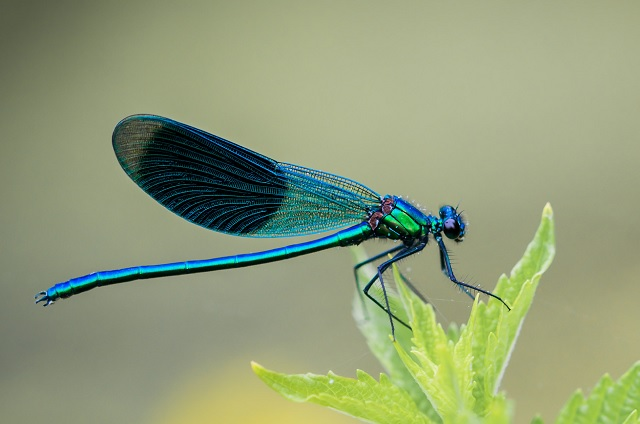
\includegraphics{pic/odonate.jpg}

\emph{Crédit photographique Pascal Boulin}

\hypertarget{le-parcours-de-formation}{%
\section*{Le parcours de formation}\label{le-parcours-de-formation}}
\addcontentsline{toc}{section}{Le parcours de formation}

Ce dispositif de formation vise à faire monter en compétence les agents du MTES (Ministère de la transition écologique et solidaire) et du MCT (Ministère de la cohésion des territoires) dans le domaine de la science de la donnée avec le logiciel R. Il est conçu pour être déployé à l'échelle nationale par le réseau des CVRH (Centre de Valorisation des Ressources Humaines).

Le parcours proposé est structuré en modules de 2 jours chacun. Les deux premiers (ou un niveau équivalent) sont des pré-requis pour suivre les suivants qui sont proposés ``à la carte'' :

\begin{enumerate}
\def\labelenumi{\arabic{enumi}.}
\tightlist
\item
  Socle : Premier programme en R
\item
  Socle : Préparation des données
\item
  Statistiques descriptives
\item
  Analyses multivariées
\item
  Datavisualisation : Produire des graphiques, des cartes et des tableaux
\item
  Documents reproductibles avec RMarkdown
\item
  Analyse spatiale\ldots{}
\end{enumerate}

et en perspective : applis interactives avec Shiny, big data, etc.

Les supports de formation sont accessibles sur la \href{https://mtes-mct.github.io/parcours-r/}{page d'accueil du parcours de formation}. Ces supports sont en \href{https://www.etalab.gouv.fr/wp-content/uploads/2017/04/ETALAB-Licence-Ouverte-v2.0.pdf}{licence ouverte}.

Si vous souhaitez accéder aux fichiers sources de ces supports, rendez-vous sur le compte \href{https://github.com/MTES-MCT?q=parcours-r}{Github du ministère}.

Pour vous tenir au courant de l'offre de formation proposée par le réseau des CVRH, \href{http://oups-cmvrh.e2.rie.gouv.fr/}{consultez la plateforme OUPS} (un accès intranet MTES-MCT est nécessaire).
Vous pouvez vous y abonner pour recevoir les annonces de formation qui vous intéressent.

Au sein du ministère, il existe une liste mail pour échanger de l'information, discuter autour de R ou encore faire part de difficultés pour trouver ensemble les solutions.
Pour s'inscrire, envoyer un message vide avec le titre ``subscribe labo.communaute-r'' à l'adresse \href{mailto:sympa@developpement-durable.gouv.fr?subject=subscribe\%20labo.communaute-r}{sympa@developpement-durable.gouv.fr}.
Il existe également un canal de discussion Ariane ouvert à tous : utilisateurs\_r, et ayant les mêmes objectifs.

Enfin,

\hypertarget{objectifs-de-ce-module}{%
\section*{Objectifs de ce module}\label{objectifs-de-ce-module}}
\addcontentsline{toc}{section}{Objectifs de ce module}

L'objectif de ce module est de présenter les éléments de manipulation des données spatiales à partir de R.
Nous verrons ainsi :

\begin{itemize}
\tightlist
\item
  Ce que sont les données spatiales
\item
  Comment lire des données spatiales ?
\item
  Comment manipuler les données spatiales ?
\item
  Comment visualiser les données spatiales ?
\end{itemize}

\hypertarget{bien-commencer}{%
\chapter{Bien commencer}\label{bien-commencer}}

\hypertarget{cruxe9er-un-projet-sous-rstudio-pour-vous-permettre-de-recenser-vos-travaux.}{%
\section{Créer un projet sous Rstudio pour vous permettre de recenser vos travaux.}\label{cruxe9er-un-projet-sous-rstudio-pour-vous-permettre-de-recenser-vos-travaux.}}

Pourquoi travailler avec les projets Rstudio plutôt que les scripts R ?

\begin{itemize}
\tightlist
\item
  Cela permet la portabilité : le répertoire de travail par défaut d'un projet est le répertoire où est ce projet. Si vous transmettez celui-ci à un collègue, le fait de lancer un programme ne dépend pas de l'arborescence de votre machine.
\end{itemize}

\begin{quote}
\textbf{Fini les \texttt{setwd("chemin/qui/marche/uniquement/sur/mon/poste")} !}
\end{quote}

\begin{itemize}
\tightlist
\item
  Toujours sur la portabilité, un projet peut être utilisé avec un package comme \texttt{renv} qui permet d'internaliser au sein du projet l'ensemble des packages utilisés dans la version utilisée. Cela permet donc à votre collègue à qui vous passez votre projet de ne pas avoir à les installer dans la même version, et si vous mettez à jour votre environnement R, votre projet restera toujours avec les versions des packages avec lesquelles vous l'avez fait tourner à l'époque. Cela évite d'avoir à subir les effets d'une mise à jour d'un package qui casserait votre code.
\end{itemize}

\texttt{renv} est intégré à Rstudio. Pour activer \texttt{renv} sur un projet, aller dans \texttt{Tools\ /\ Project\ Options\ -\textgreater{}\ Environment}

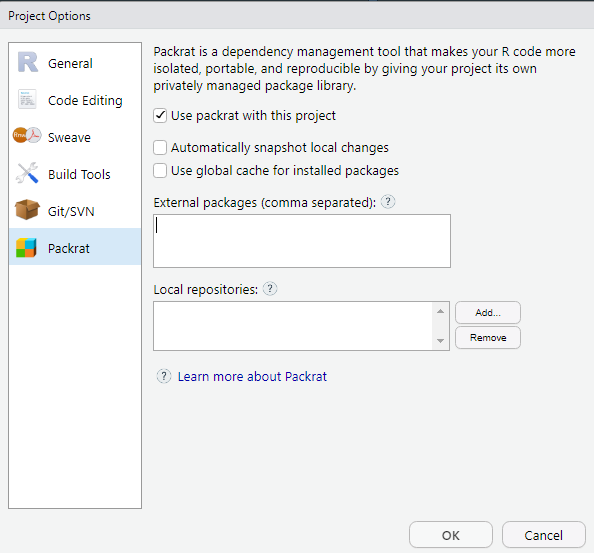
\includegraphics[width=5.20833in,height=\textheight]{pic/creerprojet4.png}

\href{https://rstudio.github.io/renv/}{En savoir plus sur renv}

\begin{itemize}
\item
  Cela permet de se forcer à travailler en mode projet : on intègre à un seul endroit tous ce qui est lié à ce projet : données brutes, données retravaillées, scripts, illustrations, documentations, publications\ldots{} et donc y compris packages avec \texttt{packrat} ou \texttt{renv}.
\item
  On peut travailler sur plusieurs projets en même temps, Rstudio ouvre alors autant de sessions que de projets.
\item
  Les projets Rstudio intègrent une interface avec les outils de gestion de version \texttt{git} et \texttt{svn.} Cela veut dire que vous pouvez versionner votre projet et l'héberger simplement comme répertoire sur des plateformes de gestion de code (forges) telle que \texttt{github} ou \texttt{gitlab}.
\end{itemize}

\textbf{Pour créer un projet : }

\begin{itemize}
\item
  Cliquez sur \emph{Project} en haut à droite puis \emph{New Project}.
  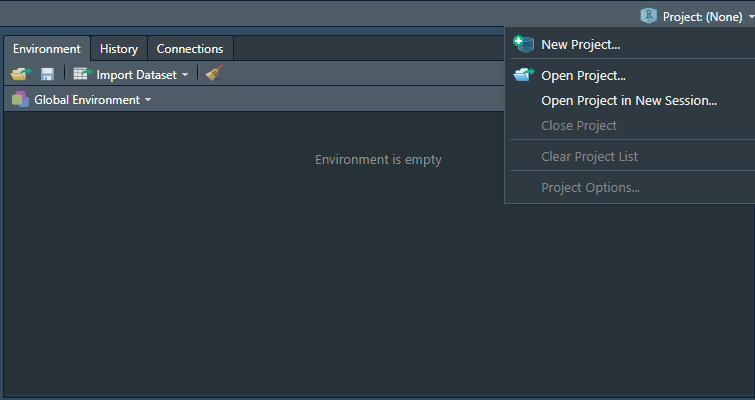
\includegraphics[width=5.20833in,height=\textheight]{pic/creerprojet1.png}
\item
  Cliquez sur \emph{New Directory}.
  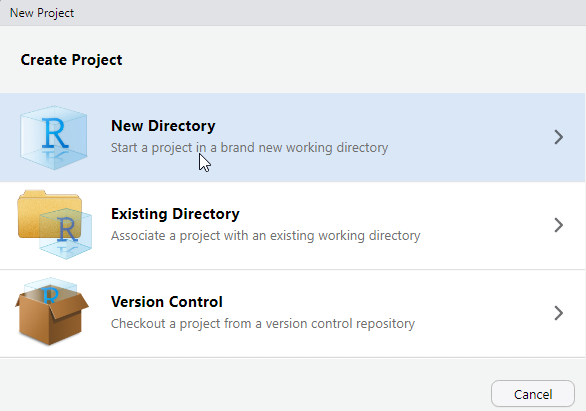
\includegraphics[width=5.20833in,height=\textheight]{pic/creerprojet2.png}
\end{itemize}

\hypertarget{duxe9sactiver-les-options-de-sauvegarde-automatique-de-rstudio}{%
\section{Désactiver les options de sauvegarde automatique de Rstudio}\label{duxe9sactiver-les-options-de-sauvegarde-automatique-de-rstudio}}

Votre code doit être reproductible depuis vos données en entrée vers votre résultat. Pour cela, il est fortement déconseillé de sauvegarder quoique ce soit dans le fichier \texttt{.RData} de sauvegarde par défaut.

Pour cela, aller dans \emph{Tools -\textgreater{} Global Options\ldots{}} et ensuite conformez vous à ceci :

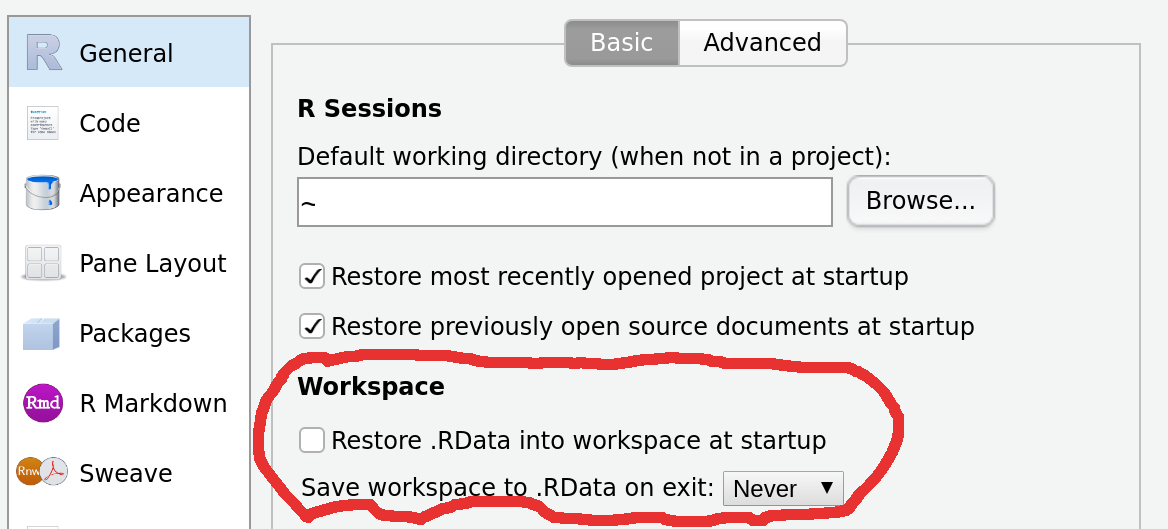
\includegraphics{pic/RData.png}

\hypertarget{intuxe9grer-vos-donnuxe9es}{%
\section{Intégrer vos données}\label{intuxe9grer-vos-donnuxe9es}}

Une bonne pratique est de créer un sous répertoire \texttt{/extdata} pour stocker les données sur lesquelles vous aurez à travailler et un dossier \texttt{/data} pour stocker les données après préparation.

Vous pouvez le faire de l'explorateur de fichier de votre système d'exploitation ou directement à partir de l'explorateur de fichier de RStudio.
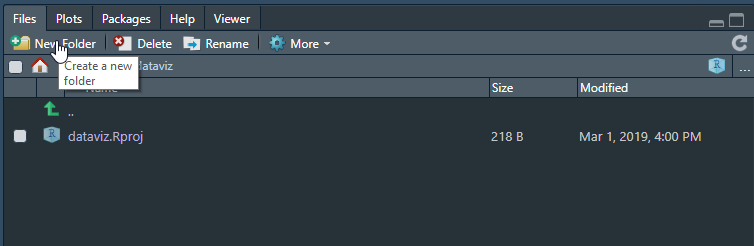
\includegraphics[width=5.20833in,height=\textheight]{pic/creerprojet3.png}

Si par la suite vous souhaitez avoir des exemples de bonnes pratiques sur comment structurer vos données, vous pouvez vous référer au \href{http://r-pkgs.had.co.nz/data.html}{chapitre data} du livre d'Hadley Wickham sur la construction de package R (tout package R étant aussi un projet !)

\hypertarget{cruxe9er-votre-arborescence-de-projet}{%
\section{Créer votre arborescence de projet}\label{cruxe9er-votre-arborescence-de-projet}}

\begin{itemize}
\item
  Créer un répertoire \texttt{/src} où vous mettrez vos scripts R.
\item
  Créer un répertoire \texttt{/figures} où vous mettrez vos illustrations issues de R.
\end{itemize}

\hypertarget{utilisation-du-package-savoirfr}{%
\section{Utilisation du package savoirfR}\label{utilisation-du-package-savoirfr}}

Pour faciliter le déroulé de ce module, l'ensemble des exercices (énoncés, corrigés et données) ont été intégrés à un package réalisé par le groupe de référent R: savoirfR

\begin{Shaded}
\begin{Highlighting}[]
\NormalTok{remotes}\SpecialCharTok{::}\FunctionTok{install\_github}\NormalTok{(}\StringTok{"MTES{-}MCT/savoirfR"}\NormalTok{)}
\end{Highlighting}
\end{Shaded}

Pour l'utiliser, il suffit de créer un nouveau projet dans un nouveau répertoire, en sélectionnant le ``Project Type'' \textbf{Exercice Parcours R MTES-MCT}.

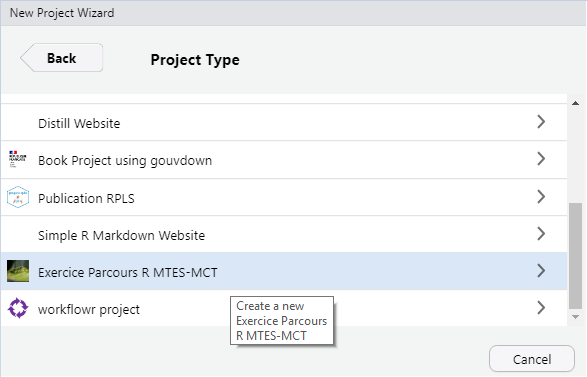
\includegraphics[width=5.20833in,height=\textheight]{pic/projetsavoirfR1.PNG}

Remplissez et sélectionnez le module suivi.

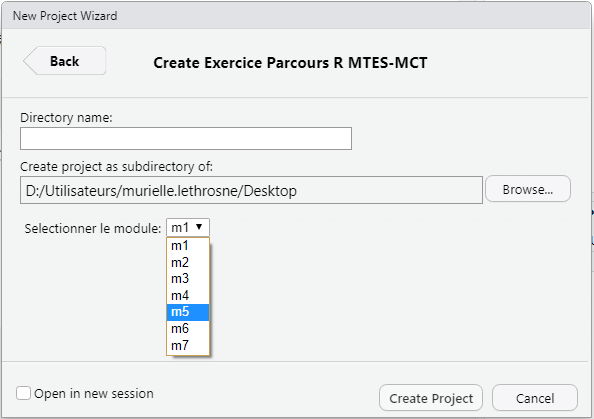
\includegraphics[width=5.20833in,height=\textheight]{pic/projetsavoirfR2.PNG}

\hypertarget{activer-les-packages-nuxe9cessaires}{%
\section{Activer les packages nécessaires}\label{activer-les-packages-nuxe9cessaires}}

Commencez par rajouter un script dans le répertoire \texttt{/src} à votre projet qui commencera par :

\begin{itemize}
\item
  activez l'ensemble des packages nécessaires,
\item
  chargez les données dont vous aurez besoin.
\end{itemize}

\begin{Shaded}
\begin{Highlighting}[]
\FunctionTok{library}\NormalTok{(cowplot)}
\FunctionTok{library}\NormalTok{(cartogram)}
\FunctionTok{library}\NormalTok{(DT)}
\FunctionTok{library}\NormalTok{(ggspatial)}
\FunctionTok{library}\NormalTok{(glue)}
\FunctionTok{library}\NormalTok{(htmlwidgets)}
\FunctionTok{library}\NormalTok{(knitr)}
\FunctionTok{library}\NormalTok{(kableExtra)}
\FunctionTok{library}\NormalTok{(leaflet)}
\FunctionTok{library}\NormalTok{(lwgeom)}
\FunctionTok{library}\NormalTok{(mapview)}
\FunctionTok{library}\NormalTok{(patchwork)}
\FunctionTok{library}\NormalTok{(rmapshaper)}
\FunctionTok{library}\NormalTok{(RPostgres)}
\FunctionTok{library}\NormalTok{(scales)}
\FunctionTok{library}\NormalTok{(sf)}
\FunctionTok{library}\NormalTok{(spData)}
\FunctionTok{library}\NormalTok{(tmap)}
\FunctionTok{library}\NormalTok{(tmaptools)}
\FunctionTok{library}\NormalTok{(tidyverse) }\CommentTok{\# comprend ggplot2, stringr, purrr, readr}
\FunctionTok{library}\NormalTok{(variousdata)}
\FunctionTok{library}\NormalTok{(viridis)}

\FunctionTok{load}\NormalTok{(}\StringTok{"extdata/admin\_express.RData"}\NormalTok{)}
\FunctionTok{load}\NormalTok{(}\StringTok{"extdata/sirene.RData"}\NormalTok{)}
\NormalTok{prefectures }\OtherTok{\textless{}{-}} \FunctionTok{read\_csv2}\NormalTok{(}\StringTok{"extdata/prefecture.csv"}\NormalTok{)}
\end{Highlighting}
\end{Shaded}

\hypertarget{bien-structurer-ses-projets-data}{%
\section{Bien structurer ses projets data}\label{bien-structurer-ses-projets-data}}

Plusieurs documents peuvent vous inspirer sur la structuration de vos projets data par la suite.

En voici quelques uns :

\begin{itemize}
\tightlist
\item
  \url{https://github.com/pavopax/new-project-template}
\item
  \url{https://nicercode.github.io/blog/2013-04-05-projects/}
\item
  \url{https://www.inwt-statistics.com/read-blog/a-meaningful-file-structure-for-r-projects.html}
\item
  \url{http://projecttemplate.net/architecture.html}
\end{itemize}

A partir du moment où quelques grands principes sont respectés (un répertoire pour les données brutes en lecture seule par exemple), le reste est surtout une question d'attirance plus forte pour l'une ou l'autre solution. L'important est de vous tenir ensuite à garder toujours la même structure dans vos projets afin de vous y retrouver plus simplement.

\hypertarget{part-introduction-aux-donnuxe9es-spatiales}{%
\part{Introduction aux données spatiales}\label{part-introduction-aux-donnuxe9es-spatiales}}

\hypertarget{la-moduxe9lisation-des-donnuxe9es-spatiales}{%
\chapter{La modélisation des données spatiales}\label{la-moduxe9lisation-des-donnuxe9es-spatiales}}

Dans ce chapitre, nous allons développer une brève introduction à la modélisation des données géographiques.

\hypertarget{les-donnuxe9es-vecteur}{%
\section{Les données vecteur}\label{les-donnuxe9es-vecteur}}

Les données vecteur sont une modélisation du monde utilisant des points, des lignes et des polygones.
Les données ``vecteur'' sont en général plus utilisées en sciences sociales, les territoires créés par l'homme ayant la plupart du temps des frontières discrètes.

Derrière les données vecteur, se trouvent des points. Les points peuvent représenter des caractéristiques autonomes (comme l'emplacement de l'établissement d'une entreprise), ou peuvent être reliés entre eux pour former des géométries plus complexes telles que des lignes (comme des cours d'eau) et des polygones (les frontières d'un pays).

Ces points sont localisés à travers un système de référence de coordonnées (CRS). La plupart des géométries ponctuelles ne contiennent que deux dimensions (les CRS à trois dimensions contiennent une valeur supplémentaire z pour la hauteur du point en référence au niveau de la mer).

\hypertarget{les-donnuxe9es-raster}{%
\section{Les données raster}\label{les-donnuxe9es-raster}}

Les données raster modélisent la surface du globe à l'aide de celulles de taille identique.
Les données ``raster'' sont en générale plus utilisées dans les science environnementales, du fait de la fiabilité des données de télédétections disponibles.

\hypertarget{la-structuration-des-donnuxe9es-guxe9ographiques-avec-r}{%
\section{La structuration des données géographiques avec R}\label{la-structuration-des-donnuxe9es-guxe9ographiques-avec-r}}

\hypertarget{sf-pour-les-donnuxe9es-vecteur}{%
\subsection{sf pour les données vecteur}\label{sf-pour-les-donnuxe9es-vecteur}}

Le packages \texttt{sf} permet de gérer les données vecteur.

Avant \texttt{sf} existait le package \texttt{sp} que vous pourrez rencontrer suivant les packages plus spécifiques que vous utiliserez ou en cherchant de l'aide.

Les avantages de \texttt{sf} sont multiples :

\begin{itemize}
\item
  \textbf{Standardisation} : sf utilise le modèle de données simple feature\footnote{\url{https://en.wikipedia.org/wiki/Simple_Features}} qui est un standard largement utilisé dans le domaine de la géomatique.
\item
  \textbf{Simplification} du modèle de données. Les données spatiales sont un \emph{dataframe} avec une variable spécifique renseignant la géométrie en créant un type ad hoc en plus des types standard (numériques, entiers, booléens, caractères, facteur\ldots). Ce dataframe aura une classe spécifique qui lui sera associée (classe \texttt{sf}).
\item
  La syntaxe des fonctions est \textbf{unifiée} et \textbf{simplifiée} selon le manifeste du tidyverse\footnote{\url{https://tidyverse.tidyverse.org/articles/manifesto.html}}.
\item
  \textbf{Intégration}. Les verbes du tidyverse sont compatibles avec les données spatiales de classe \texttt{sf} et vont parfois agir avec des propriétés spécifiques sur les données géométriques. On peut également utiliser le \emph{pipe} dans le processus de travail.
\item
  \textbf{Perfomance} : meilleure performance dans la lecture et l'écrite des données. Voir un benchmark sur la \href{https://r-spatial.github.io/sf/articles/sf1.html\#benchmarks}{page du package sf}
\end{itemize}

\hypertarget{raster-et-stars-pour-les-donnuxe9es-raster}{%
\subsection{raster et stars pour les données raster}\label{raster-et-stars-pour-les-donnuxe9es-raster}}

Les packages \texttt{raster} et \texttt{stars} permettent de gérer les données raster.

\texttt{raster} est aussi un package historique amené à être supplanté par \texttt{stars}.

\texttt{stars} est d'une part plus vaste que \texttt{raster}, car il vise à gérer les données spatio-temporelle plus largement.

\texttt{stars} est intégré à \texttt{sf} et au \texttt{tidyverse}

On se limitera pour la suite du cours aux données vecteur et donc à \texttt{sf}.

\hypertarget{les-systuxe8mes-de-coordonnuxe9es-de-ruxe9fuxe9rence}{%
\chapter{Les Systèmes de Coordonnées de Référence}\label{les-systuxe8mes-de-coordonnuxe9es-de-ruxe9fuxe9rence}}

Les données spatiales vises à modéliser la terre.
La terre est un objet dont la mesure a une longue histoire, qu'on a pensé plate, cylindrique, ronde, ellipsoïde. Maintenant, on sait que la terre a cette forme là :

THE REAL SHAPE OF PLANET EARTH - 3D Animation HD from eLearn.Punjab on Vimeo.

Les systèmes de coordonnées de référence vont permettre de se repérer sur la surface de la terre.

\hypertarget{le-systuxe8me-guxe9oduxe9sique-ou-datum}{%
\section{Le système géodésique ou datum}\label{le-systuxe8me-guxe9oduxe9sique-ou-datum}}

Pour modéliser la surface terrestre, on va définir un \emph{géoïde}, qui est la surface théorique de la pesanteur.

Ce \emph{géoïde} est proche d'un ellipsoïde, c'est à dire une surface obtenue en faisant tourner une ellipse sur son axe. La terre est en effet compressée : le rayon à l'équateur est 11,5 km plus long que le rayon polaire (Maling 1992).

On va donc pouvoir approximer ce géoïde par un ellipsoïde.

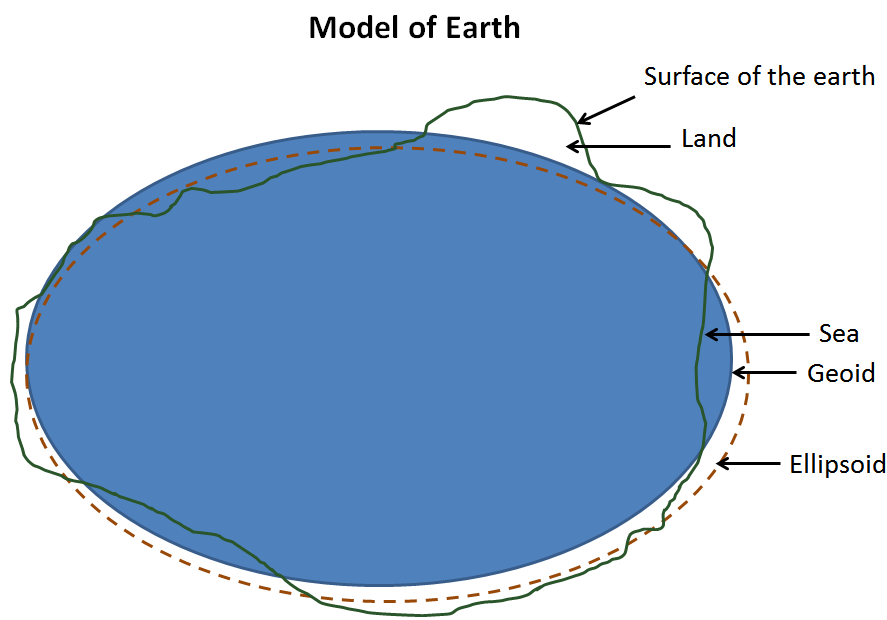
\includegraphics{pic/datum.png}

Un point quelconque est repéré par rapport à l'ellipsoïde en utilisant un système de coordonnées sphériques : longitude, latitude, altitude.

Le \emph{datum} ou \emph{système géodésique} va correspondre aux paramètre de forme de l'ellipsoïde et de positionnement sur celle ci.

On va distinguer deux types de datum : les datum \emph{locaux} et les datum \emph{globaux}.

Historiquement n'existait que des datum locaux, c'est à dire qui définissait une ellipse optimale pour correspondre à une partie déterminée de la surface de la terre. Cette contrainte était liée à la façon de définir le géoïde : avant les techniques spatiales, on utilisait des mesures de triangulation à partir d'un point défini par mesure astronomique.

\includegraphics{http://www.ngi.be/images/2/1/lokalgeodatf.gif}

Depuis l'avènement des techniques spatiales, on est capable de définir un \emph{datum global} grâce aux mesures satellitaires. Le système mondial de référence est aujourd'hui le WGS 84, associé au GPS.

Il y a donc aujourd'hui beaucoup de \emph{datum}, un pour la plupart des pays, qui maximise la modélisation de l'ellipsoïde sur leur territoire, et des datums globaux.

\hypertarget{les-coordonnuxe9es}{%
\section{Les coordonnées}\label{les-coordonnuxe9es}}

Pour se repérer sur terre, on va utiliser un système géodésique sur lequel on va se positionner avec des coordonnées.

On distingue deux types de coordonnées :

\hypertarget{coordonnuxe9es-guxe9ographiques}{%
\subsection{Coordonnées géographiques}\label{coordonnuxe9es-guxe9ographiques}}

Les systèmes de coordonnées géographiques identifient tout lieux sur la surface de la terre en utilisant deux paramètres, la longitude et la lattitude :

\begin{itemize}
\item
  La Longitude est la localisation sur la direction Est-Ouest. Elle est définie par l'angle par rapport à un méridien.
\item
  La Latitude définie la localisation sur la direction Nord-Sud. Elle est définie par l'angle avec l'équateur.
\end{itemize}

Dans un système de coordonnées géographiques, les lieux sont donc identifiés par des \emph{angles} et non des \emph{mètres}.

\hypertarget{coordonnuxe9es-en-projection}{%
\subsection{Coordonnées en projection}\label{coordonnuxe9es-en-projection}}

Les systèmes de coordonnées projetés se basent sur une modélisation de la terre plane (donc projetée sur un plan) et un système de coordonnés cartésien pour définir un point sur ce plan à partir d'une origine, d'un axe x, d'un axe y et d'une unité de mesure (comme le mètre).

Tous les systèmes de coordonnées projetés se basent sur un système de coordonnées géographiques et sur une projection spatiale des données de l'ellipse en 3D sur un plan.

Cet exercice ne peut se faire sans distorsion. Les propriétés de la surface de la terre comme l'aire, la direction, la distance, la forme ne peuvent être toutes conservées.

En général un système de coordonnées projetés ne permet de préserver qu'une ou deux de ces propriétés. On classifie d'ailleurs ces projections selon les propriétés conservées :

\begin{itemize}
\tightlist
\item
  conformes (conservent les angles)
\item
  équivalentes (conservent les surfaces)
\item
  aphylactique (peut être équidistante, c'est-à-dire conserver les distances sur les méridiens)
\end{itemize}

On distingue également les projection en fonction de leur mode de projection. Il y a trois principaux groupes de projections :

\begin{itemize}
\item
  Conique : la terre est projetée sur un cone reposant sur une ou deux tangentes. Les distorsions sont faibles sur la ligne de tangente et augmentent ensuite avec la distance à celle-ci. C'est ainsi le type de projection le mieux adapté pour des cartes réalisées sur des latitudes médianes.
\item
  Cylindrique : ces projections projettent la surface de la terre sur un cylindre. Souvent utilisées pour cartographier la terre entière.
\item
  Plane : projection du globe sur une surface plane tangeante en un point ou sur une ligne. Souvent utilisée pour les régions polaires.
\end{itemize}

\hypertarget{exemple-de-projections}{%
\subsection{Exemple de projections}\label{exemple-de-projections}}

\hypertarget{equal-earth}{%
\subsubsection{Equal Earth}\label{equal-earth}}

Le but de la projection \href{http://equal-earth.com}{Equal-Earth} est de représenter la Terre avec toutes ses régions à part égale.

Equal Earth est une projection pseudo-cylindrique ressemblant à celle de Robinson qui évoque comme elle la rotondité de la Terre. Mais à la différence de cette dernière, elle préserve les surfaces.

\begin{itemize}
\tightlist
\item
  \url{http://cartonumerique.blogspot.com/2018/11/la-projection-equal-earth.html}
\end{itemize}

\hypertarget{code-epsg}{%
\section{Code EPSG}\label{code-epsg}}

L'EPSG (European Petroleum Survey Group), un groupe créé en 1985, a défini une liste des systèmes de coordonnées géoréférencées et leur a associé des codes pour les identifier. Le groupe est devenu en 2005 le ``Comité de topographie et de positionnement'' de l'Association internationale des producteurs de pétrole et de gaz (OGP). La liste peut être trouvée sur \href{http://www.epsg.org/}{ce site}.

Un système géodésique peut recevoir plusieurs codes EPSG selon son utilisation : 2D ou 3D par exemple.

\hypertarget{part-lire-et-uxe9crire-des-donnuxe9es-spatiales}{%
\part{Lire et écrire des données spatiales}\label{part-lire-et-uxe9crire-des-donnuxe9es-spatiales}}

\hypertarget{lire-et-uxe9crire-des-donnuxe9es-spatiales-avec-r}{%
\chapter{Lire et écrire des données spatiales avec R}\label{lire-et-uxe9crire-des-donnuxe9es-spatiales-avec-r}}

Dans ce chapitre, nous allons utiliser les packages suivants :

\begin{Shaded}
\begin{Highlighting}[]
\FunctionTok{library}\NormalTok{(sf)}
\FunctionTok{library}\NormalTok{(DT)}
\FunctionTok{library}\NormalTok{(tidyverse)}
\FunctionTok{library}\NormalTok{(RPostgres)}
\FunctionTok{library}\NormalTok{(spData)}
\end{Highlighting}
\end{Shaded}

Le package \texttt{sf} s'appuie sur \texttt{GDAL} (Geospatial Data Abstraction Library) pour lire et écrire les données spatiales.

\texttt{GDAL} est une librairie permettant de lire et d'écrire des données vecteur et raster de n'importe quel format de fichier ou base de données.

Les fonctions de lecture et d'écriture de \texttt{sf} s'appellent \texttt{st\_read()} et \texttt{st\_write()}.

Pour lire des données spatiales,s \texttt{st\_read()} a besoin :

\begin{itemize}
\tightlist
\item
  d'une source de donnée : un fichier, un répertoire, une base de données ;
\item
  d'un layer: une table de données spatiale spécifique du fichier, répertoire, ou de la base de données ;
\end{itemize}

On peut avoir besoin de rajouter des options spécifiques au format de la source. Par exemple, sur des données en \texttt{csv}, il faut pouvoir spécifier la composante spatiale des données.

\hypertarget{lire-des-fichiers-plats}{%
\section{Lire des fichiers plats}\label{lire-des-fichiers-plats}}

\texttt{st\_read()} permet de lire des données spatiales disponibles en fichier plat.

Le format de fichier plat le plus populaire en géomatique est \texttt{ESRI\ Shapefile}. Ce format, en plus de ne pas être un format ouvert, a des limites bien documentées\footnote{voir \url{http://switchfromshapefile.org/}}.

Avec l'avènement du web, le format \texttt{GeoJSON} se développe beaucoup, bien qu'il soit aussi limité.

Le format considéré comme le plus prometeur est le format \texttt{OGC\ GeoPackage} promu par l'Open Geospatial Consortium\footnote{\url{https://www.geopackage.org/}}.

Mais la liste des formats lisibles par \texttt{sf} est bien plus vaste.

Pour l'obtenir, on peut utiliser \texttt{st\_drivers()}

\begin{Shaded}
\begin{Highlighting}[]
\NormalTok{DT}\SpecialCharTok{::}\FunctionTok{datatable}\NormalTok{(}\FunctionTok{st\_drivers}\NormalTok{() }\SpecialCharTok{\%\textgreater{}\%} \FunctionTok{arrange}\NormalTok{(name))}
\end{Highlighting}
\end{Shaded}

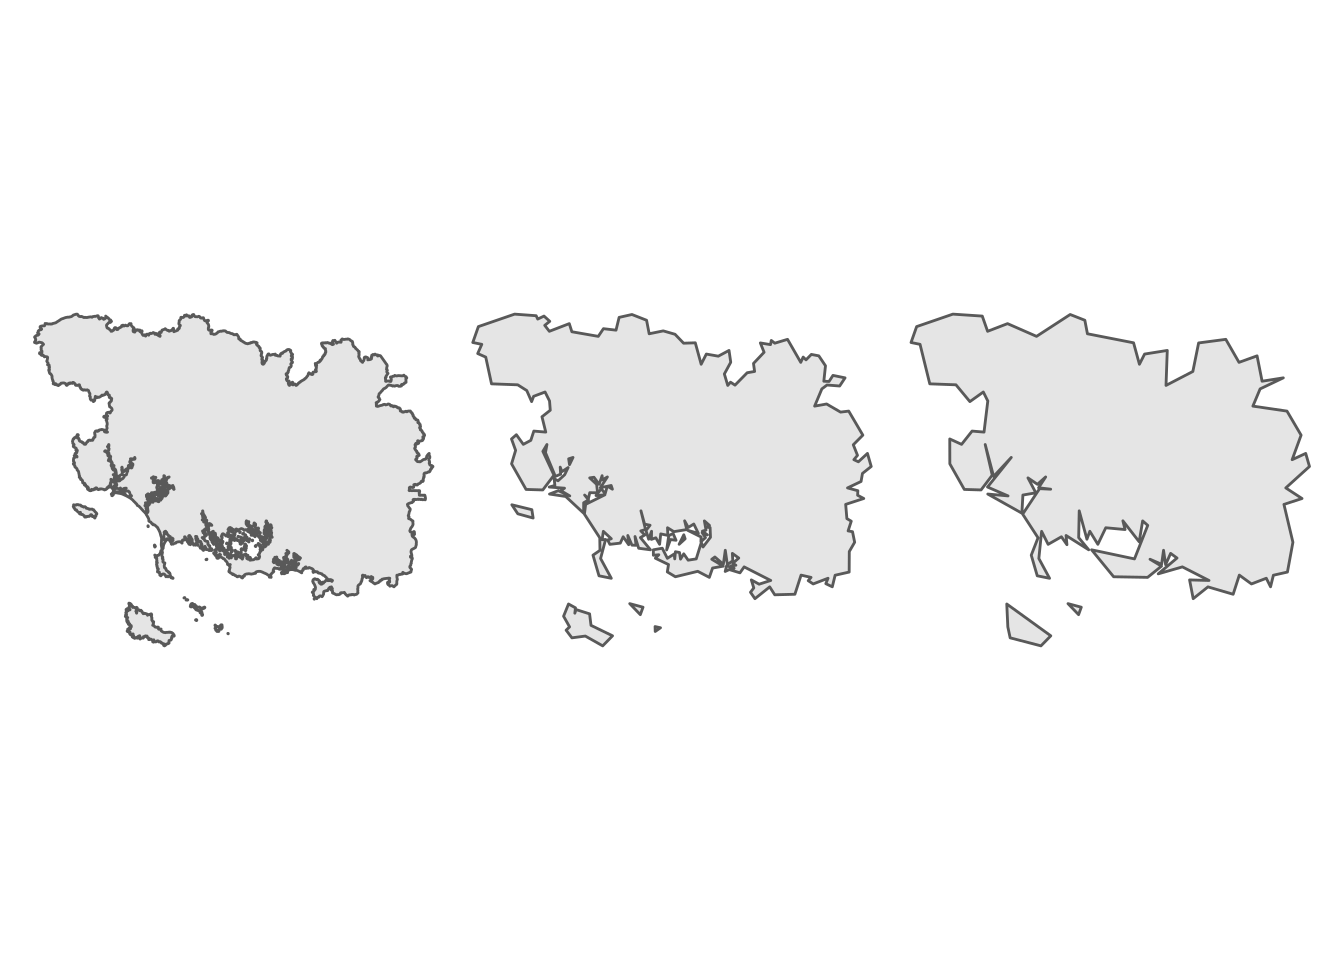
\includegraphics{support_m7_files/figure-latex/unnamed-chunk-3-1.pdf}

Exemple de lecture d'une donnée au format \texttt{GeoPackage}: les données sur la Leucémie à New York disponibles dans le package \texttt{spData}\footnote{Issues de Waller and Gotway (2004) Applied Spatial Statistics for Public Health Data.}.

\begin{Shaded}
\begin{Highlighting}[]
\NormalTok{geo\_fichier }\OtherTok{\textless{}{-}} \FunctionTok{system.file}\NormalTok{(}\StringTok{"shapes/NY8\_bna\_utm18.gpkg"}\NormalTok{, }\AttributeTok{package =} \StringTok{"spData"}\NormalTok{)}
\NormalTok{NY\_leukemia }\OtherTok{\textless{}{-}} \FunctionTok{st\_read}\NormalTok{(}\AttributeTok{dsn =}\NormalTok{ geo\_fichier)}
\end{Highlighting}
\end{Shaded}

\hypertarget{ecrire-des-fichiers-plats}{%
\section{Ecrire des fichiers plats}\label{ecrire-des-fichiers-plats}}

Ecrire des fichiers plats va se faire avec la fonction \texttt{st\_write()}.

\begin{Shaded}
\begin{Highlighting}[]
\FunctionTok{st\_write}\NormalTok{(}\AttributeTok{obj =}\NormalTok{ NY\_leukemia, }\AttributeTok{dsn =} \StringTok{"extdata/NY\_leukemia.gpkg"}\NormalTok{)}
\end{Highlighting}
\end{Shaded}

Notez que si vous cherchez à exporter une nouvelle fois ce fichier, vous aurez un message d'erreur.

Pour pouvoir écraser ce fichier, vous avez deux options :

\begin{itemize}
\tightlist
\item
  Utiliser le paramètre \texttt{layer\_option} qui vous permet d'inclure des options propres au driver utilisé.
\end{itemize}

\begin{Shaded}
\begin{Highlighting}[]
\FunctionTok{st\_write}\NormalTok{(}
  \AttributeTok{obj =}\NormalTok{ NY\_leukemia,}
  \AttributeTok{dsn =} \StringTok{"extdata/NY\_leukemia.gpkg"}\NormalTok{,}
  \AttributeTok{append =} \ConstantTok{FALSE}
\NormalTok{)}
\end{Highlighting}
\end{Shaded}

\begin{itemize}
\tightlist
\item
  Utiliser le paramètre \texttt{delete\_layer\ =\ T} de \texttt{st\_write()} qui vous permet d'écraser les layer avant sauvegarde (paramètre qui ne dépend pas du driver utilisé).
\end{itemize}

\begin{Shaded}
\begin{Highlighting}[]
\FunctionTok{st\_write}\NormalTok{(}
  \AttributeTok{obj =}\NormalTok{ NY\_leukemia,}
  \AttributeTok{dsn =} \StringTok{"extdata/NY\_leukemia.gpkg"}\NormalTok{,}
  \AttributeTok{delete\_layer =} \ConstantTok{TRUE}
\NormalTok{)}
\end{Highlighting}
\end{Shaded}

\hypertarget{lireuxe9crire-des-donnuxe9es-spatiales-sur-postgis}{%
\section{Lire/écrire des données spatiales sur PostGIS}\label{lireuxe9crire-des-donnuxe9es-spatiales-sur-postgis}}

\texttt{PostGIS}, c'est l'extension géomatique de \texttt{PostgreSQL} permettant de stocker des données géo sur un serveur de données et de les manipuler.

R va vous permettre de vous connecter simplement à une base PostGIS, pour cela vous aurez besoin du package \texttt{DBI} (package permettant de s'interfacer à des bases de données) et du package \texttt{RPostgres} (interface à PostgreSQL)

Rstudio a développé tout un site sur les interactions entre les bases de données et R, vous pouvez le trouver à l'adresse suivante : \href{https://db.rstudio.com/}{db.rstudio.com}.

Rstudio possède même depuis la version 1.1 un onglet de connexion vous permetttant de visualiser vos connexions aux bases.

Pour se connecter à une base, on va définir un driver (à quelle type de base on veut se connecter) et un connecteur (les informations de connexion).

\begin{Shaded}
\begin{Highlighting}[]
\NormalTok{drv }\OtherTok{\textless{}{-}} \FunctionTok{dbDriver}\NormalTok{(}\StringTok{"Postgres"}\NormalTok{)}
\NormalTok{con }\OtherTok{\textless{}{-}} \FunctionTok{dbConnect}\NormalTok{(drv,}
  \AttributeTok{dbname =} \StringTok{"nom\_de\_ma\_db"}\NormalTok{,}
  \AttributeTok{host =} \StringTok{"adresse\_ip\_du\_serveur"}\NormalTok{,}
  \AttributeTok{port =}\NormalTok{ numero\_du\_port,}
  \AttributeTok{user =} \StringTok{"nom\_utilisateur"}\NormalTok{,}
  \AttributeTok{password =} \StringTok{"mot\_de\_passe\_super\_secret"}
\NormalTok{)}
\end{Highlighting}
\end{Shaded}

Pour lire des données sur le serveur, on va utiliser encore la fonction \texttt{st\_read()} en lui définissant 2 paramètres : le connecteur et la requête que l'on veut réaliser.

\begin{Shaded}
\begin{Highlighting}[]
\NormalTok{ma\_table }\OtherTok{\textless{}{-}} \FunctionTok{st\_read}\NormalTok{(con, }\AttributeTok{query =} \StringTok{"SELECT * FROM le\_schema.ma\_table"}\NormalTok{)}
\end{Highlighting}
\end{Shaded}

L'avantage ici est que vous pouvez faire travailler le serveur directement sans avoir à faire travailler votre poste de travail.

Vous pouvez très bien dans cette requête sql réaliser quelques filtres, sélections et aggrégations. Celles-ci seront alors réalisées par le serveur posgreSQL et non R qui ne récupèrera que le résultat.

Vous pouvez écrire vos données ensuite de la même façon avec \texttt{st\_write()}

\begin{Shaded}
\begin{Highlighting}[]
\FunctionTok{st\_write}\NormalTok{(ma\_table,}
  \AttributeTok{dsn =}\NormalTok{ con,}
  \AttributeTok{layer =} \FunctionTok{ID}\NormalTok{(}\AttributeTok{schema =} \StringTok{"schema"}\NormalTok{, }\AttributeTok{table =} \StringTok{"ma\_table"}\NormalTok{)}
\NormalTok{)}
\end{Highlighting}
\end{Shaded}

\hypertarget{convertir-un-dataframe}{%
\section{Convertir un dataframe}\label{convertir-un-dataframe}}

Une autre façon d'obtenir un \emph{spatial dataframe} est de convertir un objet existant en objet sf. Par exemple, partir d'un dataframe sur lequel on va définir à la fois la ou les colonnes contenant la dimension géographique et le crs de référence. Ou encore convertir un objet de type \texttt{sp} en objet de type \texttt{sf}.

Pour cela, la fonction \texttt{st\_as\_sf()} permet de convertir un objet en objet \texttt{sf} en définissant la composante spatiale.

La fonction \texttt{st\_set\_crs()} permet de définir le crs de notre objet.

Exemple, nous allons lire les coordonnées géographiques des préfectures de région.

\begin{Shaded}
\begin{Highlighting}[]
\NormalTok{prefectures }\OtherTok{\textless{}{-}} \FunctionTok{read\_csv2}\NormalTok{(}\StringTok{"extdata/prefecture.csv"}\NormalTok{)}
\NormalTok{prefectures\_geo }\OtherTok{\textless{}{-}} \FunctionTok{st\_as\_sf}\NormalTok{(prefectures, }\AttributeTok{coords =} \FunctionTok{c}\NormalTok{(}\StringTok{"x"}\NormalTok{, }\StringTok{"y"}\NormalTok{)) }\SpecialCharTok{\%\textgreater{}\%}
  \FunctionTok{st\_set\_crs}\NormalTok{(}\DecValTok{2154}\NormalTok{)}
\end{Highlighting}
\end{Shaded}

\hypertarget{part-manipuler-des-donnuxe9es-spatiales}{%
\part{Manipuler des données spatiales}\label{part-manipuler-des-donnuxe9es-spatiales}}

\hypertarget{les-opuxe9rations-sur-donnuxe9es-attributaires}{%
\chapter{Les opérations sur données attributaires}\label{les-opuxe9rations-sur-donnuxe9es-attributaires}}

Dans ce chapitre, nous allons utiliser les packages suivants :

\begin{Shaded}
\begin{Highlighting}[]
\FunctionTok{library}\NormalTok{(sf)}
\FunctionTok{library}\NormalTok{(tidyverse)}
\FunctionTok{library}\NormalTok{(mapview)}
\end{Highlighting}
\end{Shaded}

Nous utiliserons les contours des territoires de la France métropolitaine issus de Admin Express.

\begin{Shaded}
\begin{Highlighting}[]
\FunctionTok{load}\NormalTok{(}\StringTok{"extdata/admin\_express.RData"}\NormalTok{)}
\end{Highlighting}
\end{Shaded}

Prenons la table des départements, cette table est un \texttt{spatial\ dataframe}.

\begin{Shaded}
\begin{Highlighting}[]
\FunctionTok{class}\NormalTok{(departements\_geo)}
\end{Highlighting}
\end{Shaded}

\begin{verbatim}
[1] "sf"         "data.frame"
\end{verbatim}

On peut utiliser \texttt{mapview()} pour voir ce jeu de données.

\begin{Shaded}
\begin{Highlighting}[]
\FunctionTok{mapview}\NormalTok{(departements\_geo, }\AttributeTok{zcol =} \StringTok{"NOM\_DEP"}\NormalTok{, }\AttributeTok{legend =} \ConstantTok{FALSE}\NormalTok{)}
\end{Highlighting}
\end{Shaded}

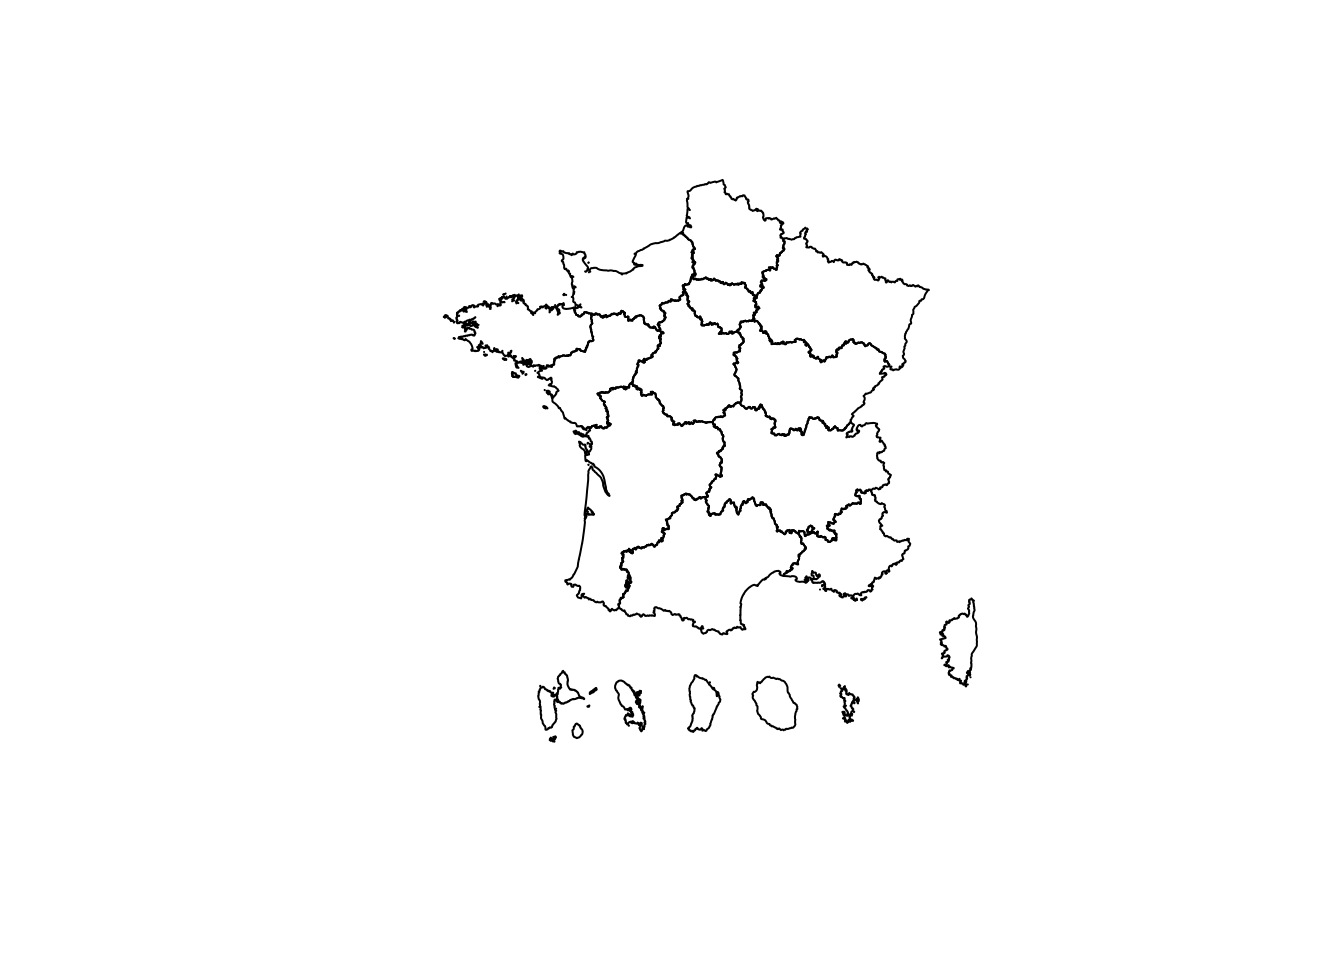
\includegraphics{support_m7_files/figure-latex/unnamed-chunk-15-1.pdf}

Comme évoqué dans la partie 1, on peut tout à fait appliquer sur un \texttt{spatial\ dataframe} les verbes du \texttt{tidyverse} comme sur un \texttt{dataframe}, notamment utiliser les verbes de \texttt{dplyr}.

Nous pouvons à partir de cette table filtrer les départements d'une certaine région.

\begin{Shaded}
\begin{Highlighting}[]
\NormalTok{departements\_geo }\SpecialCharTok{\%\textgreater{}\%}
  \FunctionTok{filter}\NormalTok{(INSEE\_REG }\SpecialCharTok{==} \DecValTok{52}\NormalTok{)}
\end{Highlighting}
\end{Shaded}

\begin{verbatim}
Simple feature collection with 5 features and 5 fields
Geometry type: MULTIPOLYGON
Dimension:     XY
Bounding box:  xmin: 276225 ymin: 6582682 xmax: 545050 ymax: 6834664
Projected CRS: RGF93 / Lambert-93
                        ID          NOM_DEP INSEE_DEP INSEE_REG
1 DEP000000000000000000045 LOIRE-ATLANTIQUE        44        52
2 DEP000000000000000000050   MAINE-ET-LOIRE        49        52
3 DEP000000000000000000054          MAYENNE        53        52
4 DEP000000000000000000073           SARTHE        72        52
5 DEP000000000000000000086           VENDEE        85        52
              AREA                       geometry
1 6996715678 [m^2] MULTIPOLYGON (((276339 6716...
2 7160501206 [m^2] MULTIPOLYGON (((419761 6744...
3 5207890788 [m^2] MULTIPOLYGON (((398109 6788...
4 6238251339 [m^2] MULTIPOLYGON (((463283 6791...
5 6760370737 [m^2] MULTIPOLYGON (((293744 6673...
\end{verbatim}

Nous pouvons ne sélectionner que quelques variables

\begin{Shaded}
\begin{Highlighting}[]
\NormalTok{departements\_geo }\SpecialCharTok{\%\textgreater{}\%}
  \FunctionTok{select}\NormalTok{(INSEE\_DEP) }\SpecialCharTok{\%\textgreater{}\%}
  \FunctionTok{glimpse}\NormalTok{()}
\end{Highlighting}
\end{Shaded}

\begin{verbatim}
Rows: 96
Columns: 2
$ INSEE_DEP <fct> 01, 2B, 02, 2A, 03, 04, 05, 06, 07, 08, 09, 10, 11, 12, 13, ~
$ geometry  <MULTIPOLYGON [m]> MULTIPOLYGON (((839096 6563..., MULTIPOLYGON ((~
\end{verbatim}

A noter que par défaut, un \texttt{spatial\ dataframe} gardera toujours la géométrie.

Nous pouvons agréger nos données.

\begin{Shaded}
\begin{Highlighting}[]
\NormalTok{regions }\OtherTok{\textless{}{-}}\NormalTok{ departements\_geo }\SpecialCharTok{\%\textgreater{}\%}
  \FunctionTok{group\_by}\NormalTok{(INSEE\_REG) }\SpecialCharTok{\%\textgreater{}\%}
  \FunctionTok{summarise}\NormalTok{(}\AttributeTok{AREA =} \FunctionTok{sum}\NormalTok{(AREA))}

\FunctionTok{glimpse}\NormalTok{(regions)}
\end{Highlighting}
\end{Shaded}

\begin{verbatim}
Rows: 13
Columns: 3
$ INSEE_REG <fct> 11, 24, 27, 28, 32, 44, 52, 53, 75, 76, 84, 93, 94
$ AREA      [m^2] 12064378723 [m^2], 39470054055 [m^2], 47980260943 [m^2], 301~
$ geometry  <GEOMETRY [m]> POLYGON ((670090 6886753, 6..., POLYGON ((625482 6798942, 6.~
\end{verbatim}

On voit que \texttt{summarise} permet non seulement d'agréger nos données attributaires, mais également les géométries.

Cette opération permet donc de retrouver directement notre carte des régions métropolitaines.

\begin{Shaded}
\begin{Highlighting}[]
\FunctionTok{mapview}\NormalTok{(regions, }\AttributeTok{zcol =} \StringTok{"INSEE\_REG"}\NormalTok{, }\AttributeTok{legend =}\NormalTok{ F)}
\end{Highlighting}
\end{Shaded}

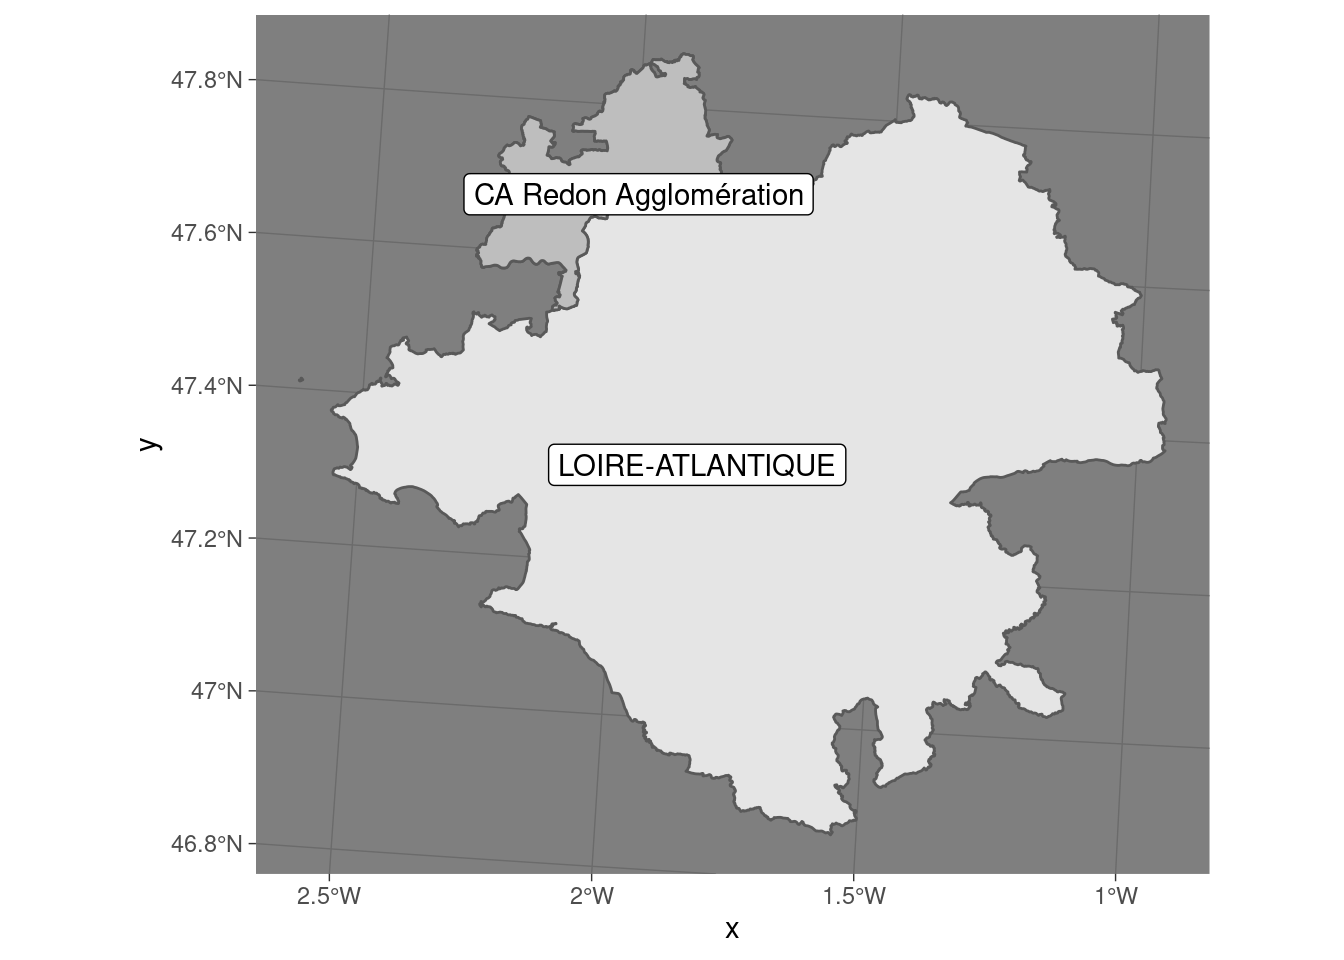
\includegraphics{support_m7_files/figure-latex/unnamed-chunk-19-1.pdf}

On peut enfin effectuer des jointures attributaines sur nos données en utilisant les verbes à deux dataframe de \texttt{dplyr}.

Par exemple on va pouvoir récupérer, dans la table \texttt{regions\_geo} de notre \texttt{RData}, les libellées de nos régions.

\begin{Shaded}
\begin{Highlighting}[]
\NormalTok{regions }\OtherTok{\textless{}{-}}\NormalTok{ regions }\SpecialCharTok{\%\textgreater{}\%}
  \FunctionTok{left\_join}\NormalTok{(regions\_geo }\SpecialCharTok{\%\textgreater{}\%}
    \FunctionTok{st\_drop\_geometry}\NormalTok{(),}
  \AttributeTok{by =} \FunctionTok{c}\NormalTok{(}\StringTok{"INSEE\_REG"}\NormalTok{)}
\NormalTok{  )}
\end{Highlighting}
\end{Shaded}

Nous pouvons alors utiliser ce nouvelle attribut pour nos cartes.

\begin{Shaded}
\begin{Highlighting}[]
\FunctionTok{mapview}\NormalTok{(regions, }\AttributeTok{zcol =} \StringTok{"NOM\_REG"}\NormalTok{, }\AttributeTok{legend =}\NormalTok{ F)}
\end{Highlighting}
\end{Shaded}

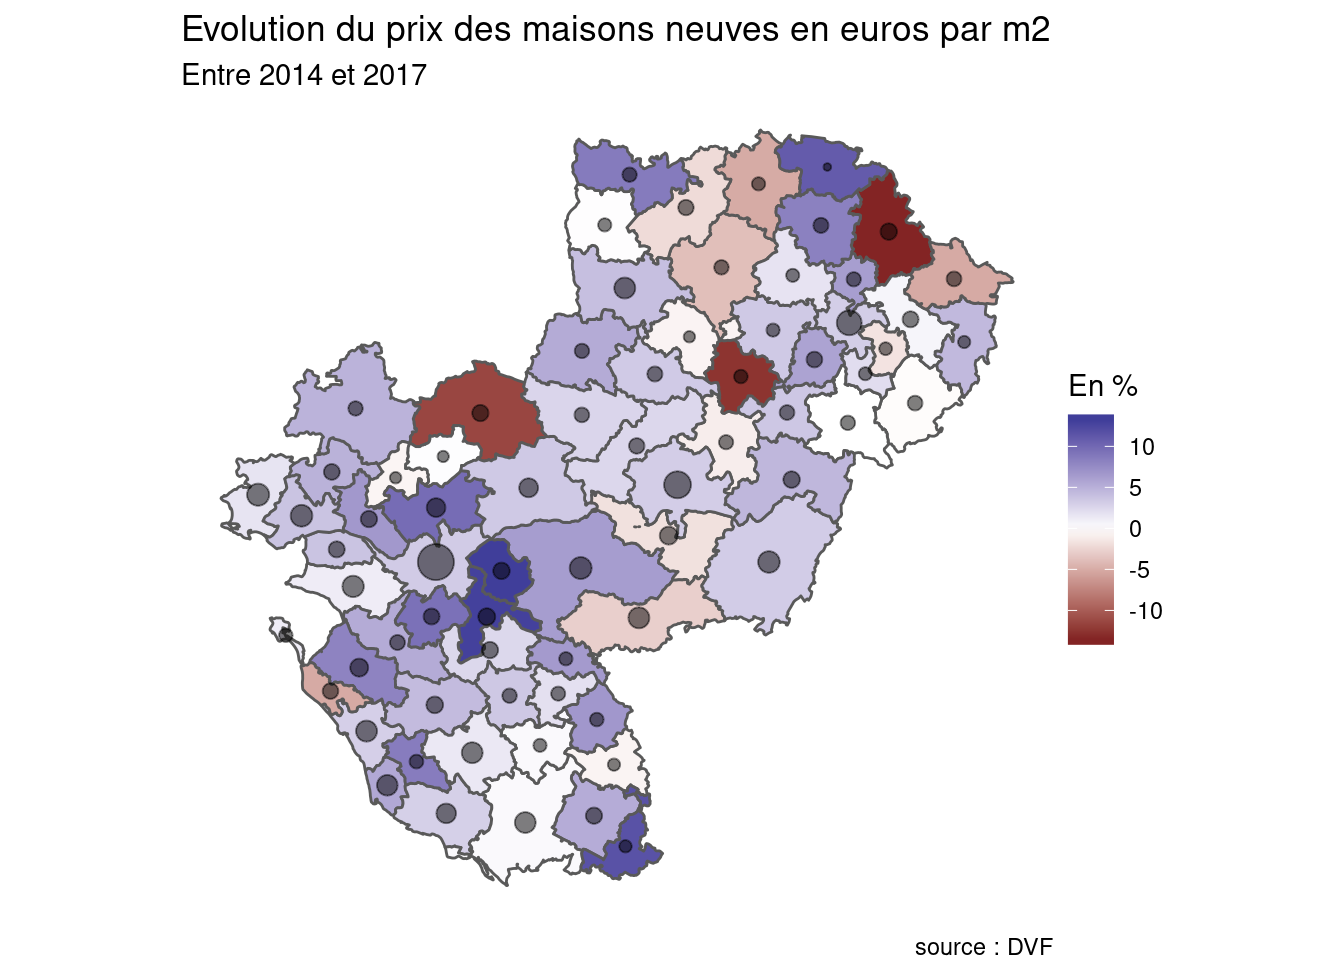
\includegraphics{support_m7_files/figure-latex/unnamed-chunk-21-1.pdf}

\begin{rmdnote}
Attention, quand vous réalisez une jointure entre deux tables de données
:

X \%\textgreater\% ZZ\_join(Y)

La composante spatiale n'est conservée que pour la première table X.
\end{rmdnote}

\hypertarget{les-opuxe9rations-spatiales-sur-les-donnuxe9es}{%
\chapter{Les opérations spatiales sur les données}\label{les-opuxe9rations-spatiales-sur-les-donnuxe9es}}

Les opérations spatiales sont des opérations prenant nos données en entrée pour en sortir un résultat dépendant de leur composante spatiale (forme, localisation).

Dans ce chapitre, nous allons utiliser les packages suivants.

\begin{Shaded}
\begin{Highlighting}[]
\FunctionTok{library}\NormalTok{(sf)}
\FunctionTok{library}\NormalTok{(tidyverse)}
\FunctionTok{library}\NormalTok{(mapview)}
\FunctionTok{library}\NormalTok{(ggplot2)}
\end{Highlighting}
\end{Shaded}

Nous utiliserons les données de la table des régions de la France métropolitaine et des établissements publics de coopération intercommunale (EPCI)\footnote{\url{https://fr.wikipedia.org/wiki/\%C3\%89tablissement_public_de_coop\%C3\%A9ration_intercommunale}} de la France Métropolitaine

\begin{Shaded}
\begin{Highlighting}[]
\FunctionTok{load}\NormalTok{(}\StringTok{"extdata/admin\_express.RData"}\NormalTok{)}
\end{Highlighting}
\end{Shaded}

\begin{Shaded}
\begin{Highlighting}[]
\FunctionTok{glimpse}\NormalTok{(epci\_geo)}
\end{Highlighting}
\end{Shaded}

\begin{verbatim}
Rows: 1,241
Columns: 5
$ ID        <fct> EPCI00000000000000000001, EPCI00000000000000000002, EPCI0000~
$ CODE_EPCI <fct> 200000172, 200000438, 200000545, 200000628, 200000800, 20000~
$ NOM_EPCI  <fct> "CC Faucigny-Glières", "CC du Pays de Pontchâteau Saint-Gild~
$ TYPE_EPCI <fct> CC, CC, CC, CC, CC, CC, CC, CC, CC, CC, CA, CC, CC, CC, CC, ~
$ geometry  <MULTIPOLYGON [m]> MULTIPOLYGON (((964676 6561..., MULTIPOLYGON ((~
\end{verbatim}

\begin{Shaded}
\begin{Highlighting}[]
\FunctionTok{glimpse}\NormalTok{(departements\_geo)}
\end{Highlighting}
\end{Shaded}

\begin{verbatim}
Rows: 96
Columns: 6
$ ID        <fct> DEP000000000000000000001, DEP000000000000000000002, DEP00000~
$ NOM_DEP   <fct> AIN, HAUTE-CORSE, AISNE, CORSE-DU-SUD, ALLIER, ALPES-DE-HAUT~
$ INSEE_DEP <fct> 01, 2B, 02, 2A, 03, 04, 05, 06, 07, 08, 09, 10, 11, 12, 13, ~
$ INSEE_REG <fct> 84, 94, 32, 94, 84, 93, 93, 93, 84, 44, 76, 44, 76, 76, 93, ~
$ AREA      [m^2] 5774813521 [m^2], 4722274798 [m^2], 7419025664 [m^2], 403749~
$ geometry  <MULTIPOLYGON [m]> MULTIPOLYGON (((839096 6563..., MULTIPOLYGON ((~
\end{verbatim}

\begin{Shaded}
\begin{Highlighting}[]
\FunctionTok{glimpse}\NormalTok{(regions\_geo)}
\end{Highlighting}
\end{Shaded}

\begin{verbatim}
Rows: 13
Columns: 4
$ ID        <fct> REG000000000000000000001, REG000000000000000000002, REG00000~
$ NOM_REG   <fct> AUVERGNE-RHONE-ALPES, BOURGOGNE-FRANCHE-COMTE, BRETAGNE, CEN~
$ INSEE_REG <fct> 84, 27, 53, 24, 94, 44, 32, 11, 28, 75, 76, 52, 93
$ geometry  <MULTIPOLYGON [m]> MULTIPOLYGON (((974065 6594..., MULTIPOLYGON (((880573 6730.~
\end{verbatim}

\hypertarget{filtrer}{%
\section{Filtrer}\label{filtrer}}

Nous souhaitons par exemple filtrer nos EPCI sur les EPCI du département de Loire-Atlantique.

\begin{Shaded}
\begin{Highlighting}[]
\NormalTok{departement\_44 }\OtherTok{\textless{}{-}}\NormalTok{ departements\_geo }\SpecialCharTok{\%\textgreater{}\%}
  \FunctionTok{filter}\NormalTok{(INSEE\_DEP }\SpecialCharTok{==} \StringTok{"44"}\NormalTok{)}

\NormalTok{epci\_d44 }\OtherTok{\textless{}{-}}\NormalTok{ epci\_geo[departement\_44, , op }\OtherTok{=}\NormalTok{ st\_within]}

\FunctionTok{mapview}\NormalTok{(}\FunctionTok{list}\NormalTok{(departement\_44, epci\_d44), }\AttributeTok{zcol =} \FunctionTok{list}\NormalTok{(}\StringTok{"NOM\_DEP"}\NormalTok{, }\StringTok{"NOM\_EPCI"}\NormalTok{), }\AttributeTok{legend =}\NormalTok{ F)}
\end{Highlighting}
\end{Shaded}

\includegraphics{support_m7_files/figure-latex/unnamed-chunk-28-1.pdf}

L'opération de filtre sur les données spatiales fonctionne en prenant la table en entrée (\texttt{epci\_geo}), la table avec laquelle on souhaite définir les lignes à garder (\texttt{departement\_44}),et l'opérateur qui va définir le test entre les deux géométries. Ici cet opérateur est \texttt{st\_within(x,y)}, qui renvoie \texttt{TRUE} si la géométrie de \texttt{x} est contenue à l'intérieur de celle de \texttt{y}.

On peut spécifier différents prédicats spatiaux pour réaliser ce filtre.

En deuxième argument (\texttt{,\ ,}), on peut rajouter, comme dans une opération \texttt{{[}} classique de R les colonnes que l'on souhaite garder.

On voit ici que le résultat n'est pas très concluant : il manque 3 epci du département, ceux qui sortent des frontières de celui-ci.
Prenons un buffer autour du département.

\begin{rmdnote}
Qu'est ce qu'un buffer ? C'est un tampon qui va nous permettre d'appliquer une transformation sur un objet vectoriel.

A partir d'une couche de départ de type ponctuel, linéaire ou polygonal, le buffer va créer une nouvelle couche vectorielle. La géométrie de cette couche représente des objets surfaciques dont les frontières sont positionnées à une distance euclidienne, définie par l'utilisateur, des limites des objets vectoriels de la couche de départ.
\end{rmdnote}

La fonction qui permet de faire cela avec \texttt{sf} s'appelle \texttt{st\_buffer()}.

\texttt{st\_buffer()} prend en paramètre :

\begin{itemize}
\tightlist
\item
  un objet de classe \emph{sf}
\item
  une distance dont l'unité est définie par celle de l'objet \texttt{sf}, que l'on peut obtenir comme ceci \texttt{st\_crs(x)\$units}.
\end{itemize}

\begin{Shaded}
\begin{Highlighting}[]
\NormalTok{departement\_44\_buffer }\OtherTok{\textless{}{-}}\NormalTok{ departement\_44 }\SpecialCharTok{\%\textgreater{}\%}
  \FunctionTok{st\_buffer}\NormalTok{(}\AttributeTok{dist =} \DecValTok{5000}\NormalTok{)}

\FunctionTok{mapview}\NormalTok{(}\FunctionTok{list}\NormalTok{(departement\_44\_buffer, departement\_44), }\AttributeTok{layer.name =} \FunctionTok{c}\NormalTok{(}\StringTok{"Loire{-}Atlantique avec un buffer de 5 km"}\NormalTok{, }\StringTok{"Loire{-}Atlantique"}\NormalTok{), }\AttributeTok{zcol =} \FunctionTok{list}\NormalTok{(}\StringTok{"NOM\_DEP"}\NormalTok{, }\StringTok{"NOM\_DEP"}\NormalTok{), }\AttributeTok{col.regions =} \FunctionTok{list}\NormalTok{(}\StringTok{"\#440154FF"}\NormalTok{, }\StringTok{"\#FDE725FF"}\NormalTok{), }\AttributeTok{legend =} \ConstantTok{FALSE}\NormalTok{)}
\end{Highlighting}
\end{Shaded}

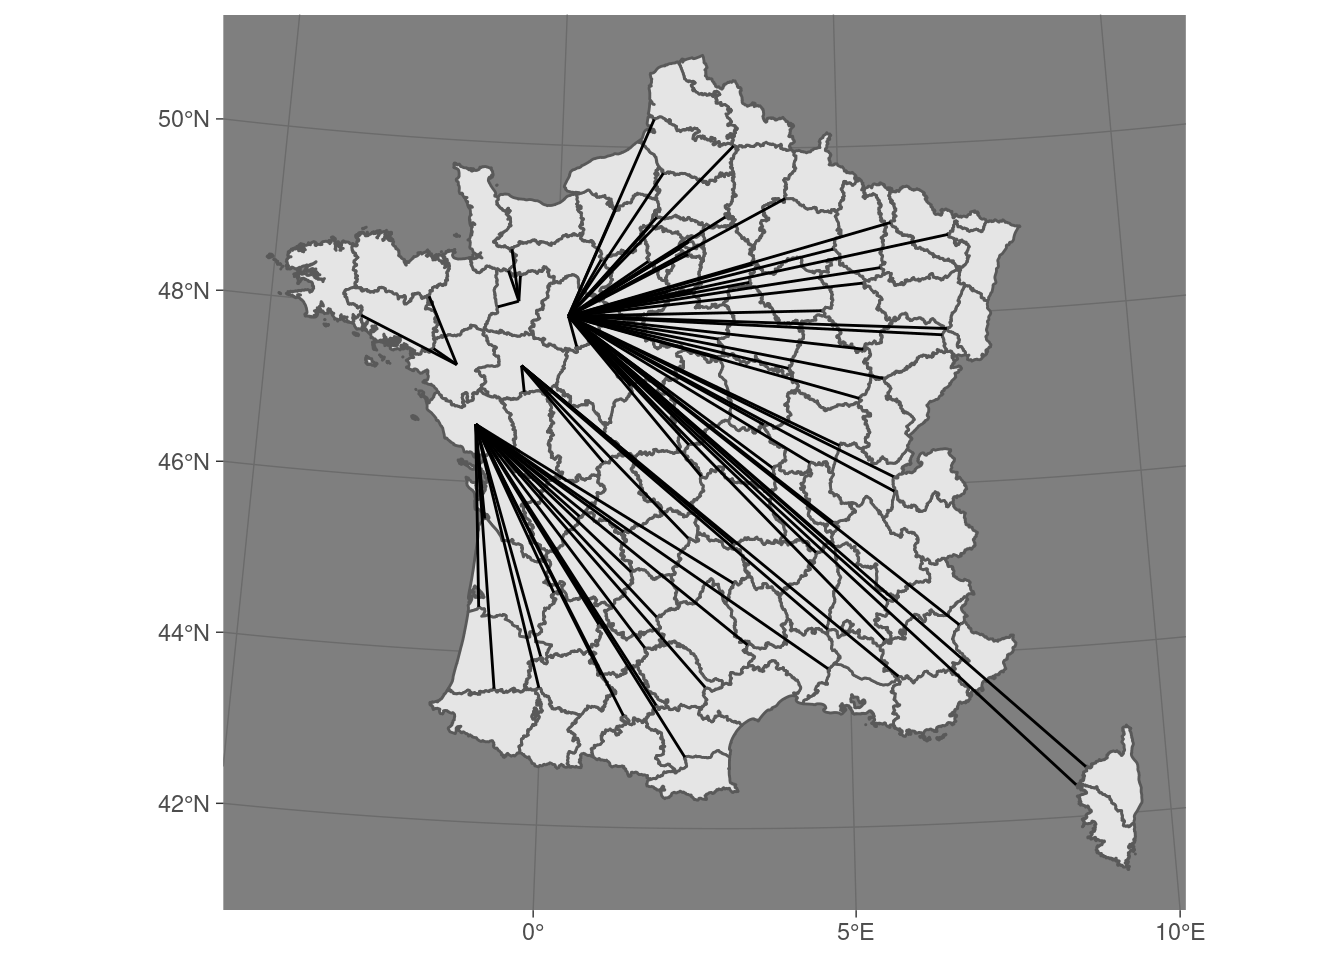
\includegraphics{support_m7_files/figure-latex/unnamed-chunk-30-1.pdf}

\begin{Shaded}
\begin{Highlighting}[]
\NormalTok{epci\_d44\_buffer }\OtherTok{\textless{}{-}}\NormalTok{ epci\_geo[departement\_44\_buffer, , op }\OtherTok{=}\NormalTok{ st\_within]}

\FunctionTok{mapview}\NormalTok{(}\FunctionTok{list}\NormalTok{(departement\_44\_buffer, epci\_d44\_buffer), }\AttributeTok{zcol =} \FunctionTok{list}\NormalTok{(}\StringTok{"NOM\_DEP"}\NormalTok{, }\StringTok{"NOM\_EPCI"}\NormalTok{), }\AttributeTok{legend =}\NormalTok{ F)}
\end{Highlighting}
\end{Shaded}

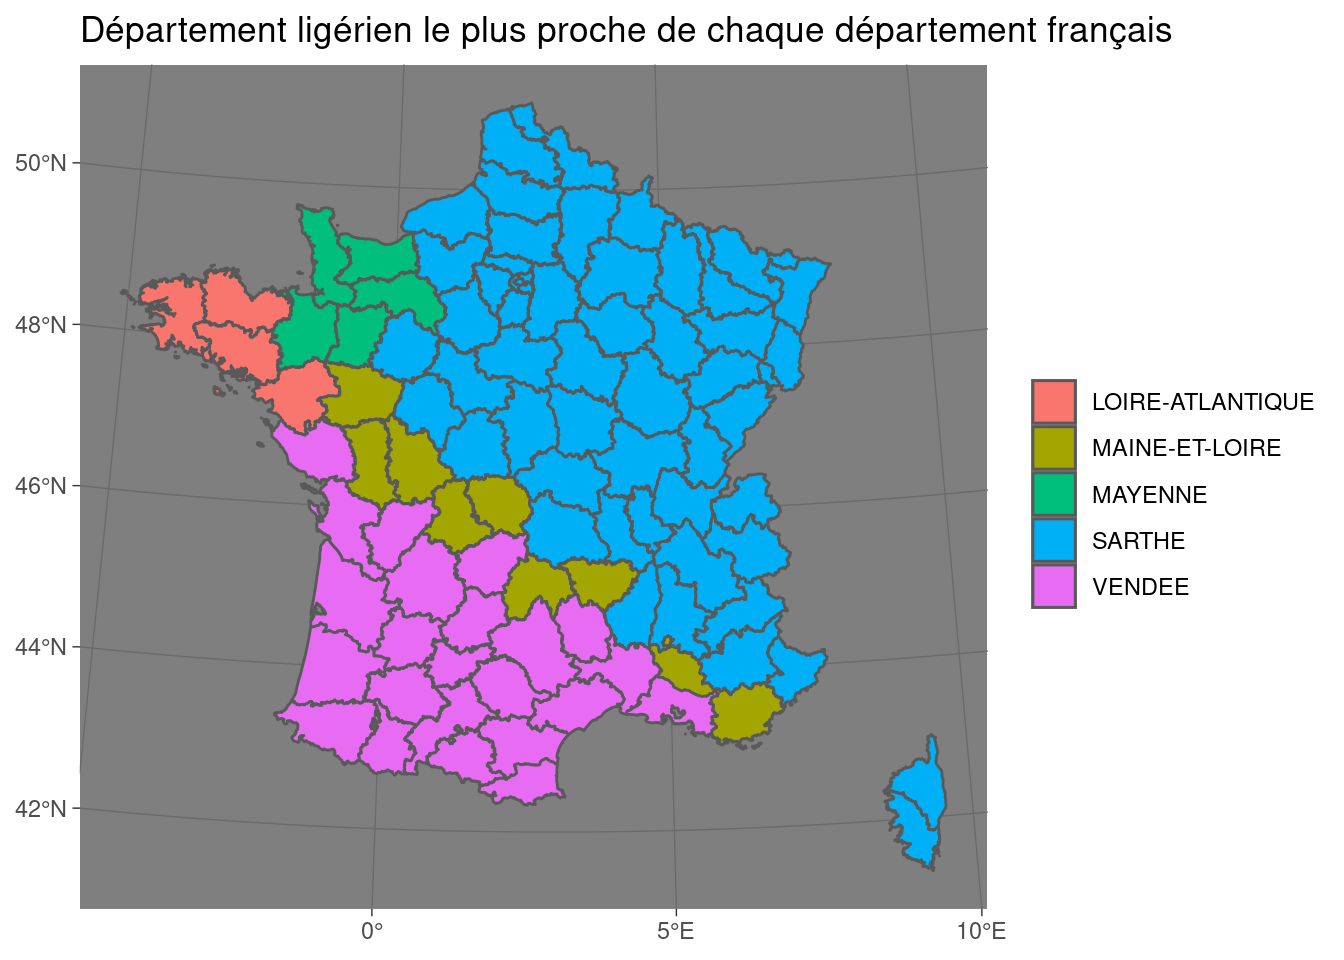
\includegraphics{support_m7_files/figure-latex/unnamed-chunk-31-1.pdf}

On récupère 2 des 3 epci manquant ainsi. Celui qui manque est l'Epci de Redon qui est à cheval sur la Loire-Atlantique, le Morbihan et l'Ile et Vilaine.
Une méthode pour le récupérer est de prendre l'opérateur de filtre \texttt{st\_intersect} au lieu de \texttt{st\_within} en utilisant un buffer légèrement négatif de notre département pour ne pas récupérer les epci limitrophes.

\begin{Shaded}
\begin{Highlighting}[]
\NormalTok{departement\_44\_buffer\_negatif }\OtherTok{\textless{}{-}}\NormalTok{ departement\_44 }\SpecialCharTok{\%\textgreater{}\%}
  \FunctionTok{st\_buffer}\NormalTok{(}\AttributeTok{dist =} \SpecialCharTok{{-}}\DecValTok{2000}\NormalTok{)}

\NormalTok{epci\_d44 }\OtherTok{\textless{}{-}}\NormalTok{ epci\_geo[departement\_44\_buffer\_negatif, , op }\OtherTok{=}\NormalTok{ st\_intersects]}

\FunctionTok{mapview}\NormalTok{(}\FunctionTok{list}\NormalTok{(departement\_44, epci\_d44), }\AttributeTok{zcol =} \FunctionTok{list}\NormalTok{(}\StringTok{"NOM\_DEP"}\NormalTok{, }\StringTok{"NOM\_EPCI"}\NormalTok{), }\AttributeTok{legend =}\NormalTok{ F)}
\end{Highlighting}
\end{Shaded}

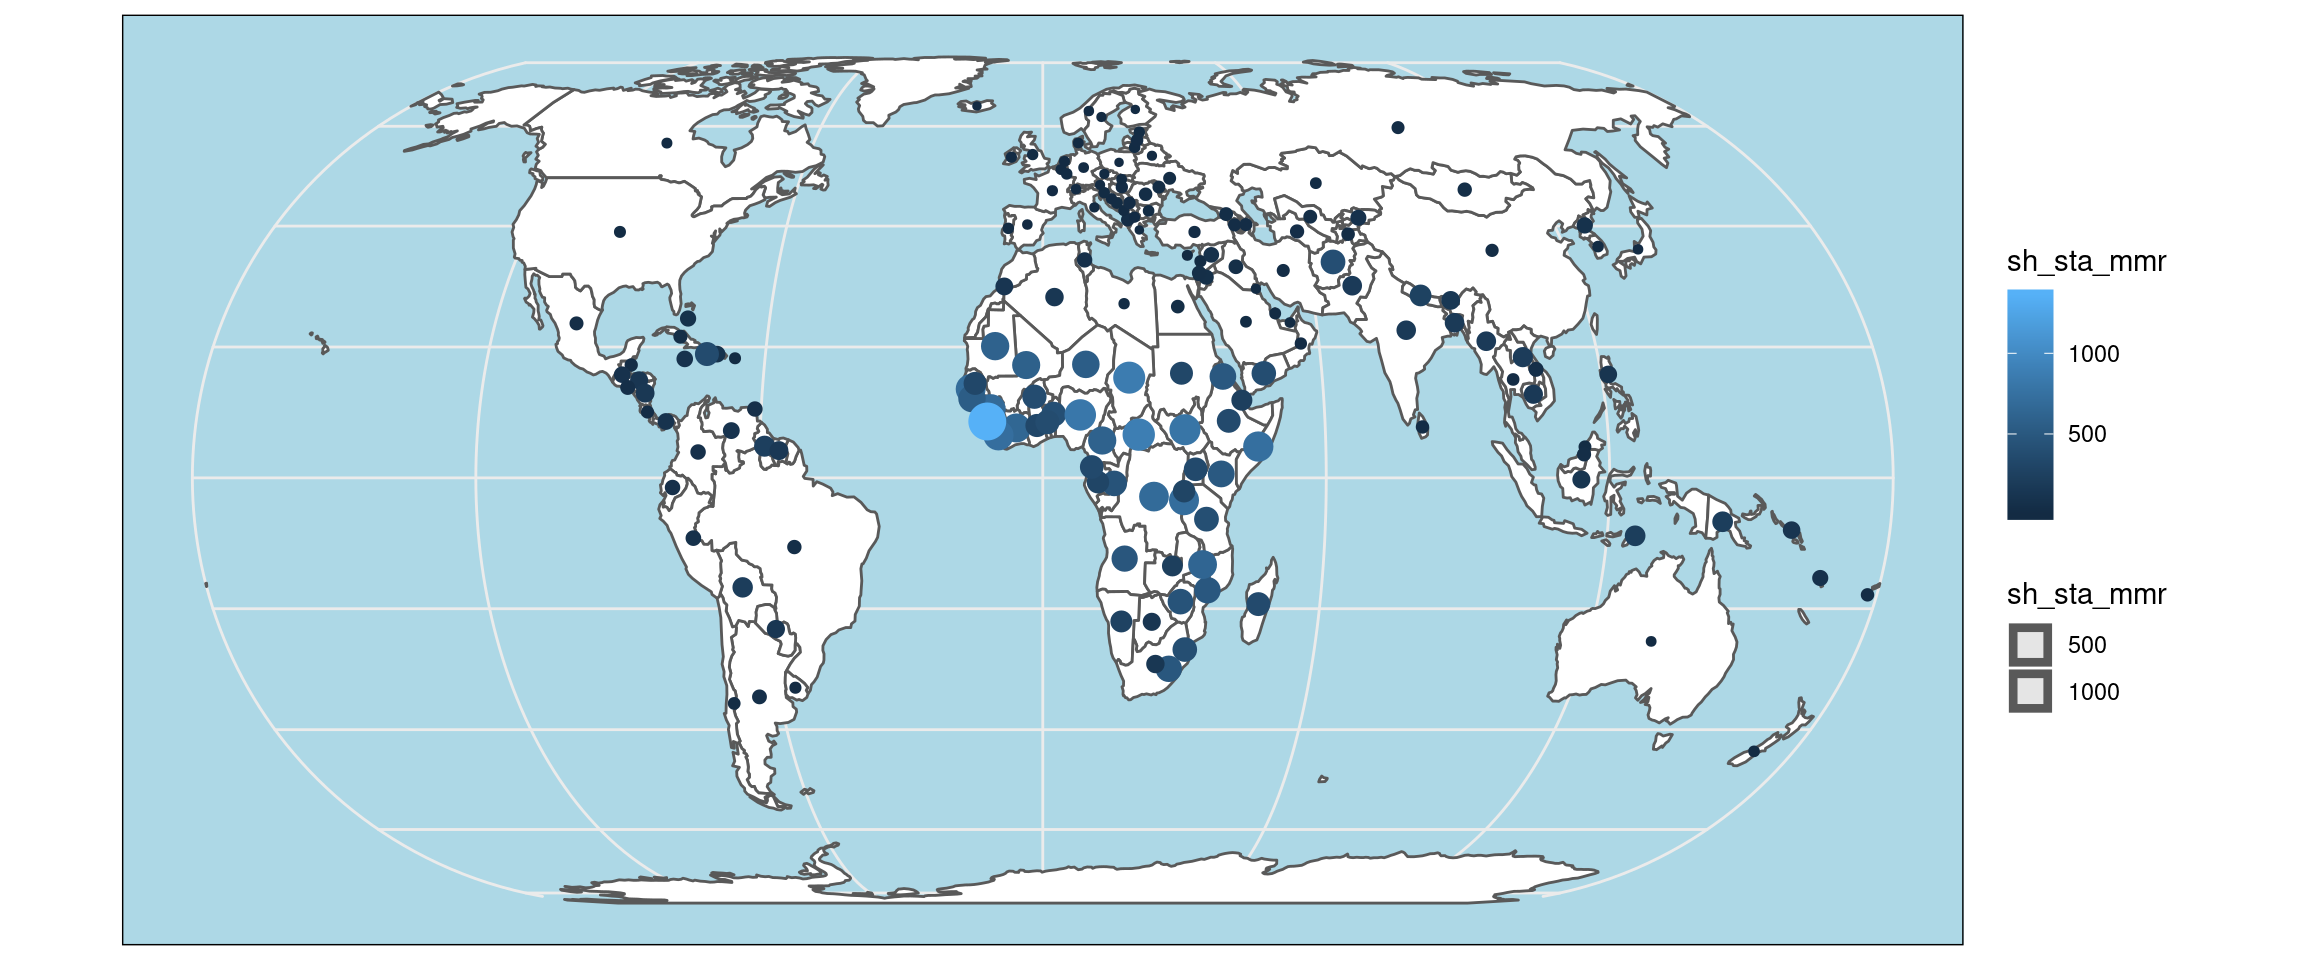
\includegraphics{support_m7_files/figure-latex/unnamed-chunk-32-1.pdf}

\hypertarget{pruxe9dicats-spatiaux}{%
\section{Prédicats spatiaux}\label{pruxe9dicats-spatiaux}}

Les prédicats spatiaux décrivent les relations spatiales entre objets. Pour bien les illustrer on va utiliser quelques données de test.
Nous allons utiliser un polygone (a), des lignes (l) et des points (p).

\begin{Shaded}
\begin{Highlighting}[]
\CommentTok{\# polygone (a)}
\NormalTok{a\_poly }\OtherTok{\textless{}{-}} \FunctionTok{st\_polygon}\NormalTok{(}\FunctionTok{list}\NormalTok{(}\FunctionTok{rbind}\NormalTok{(}\FunctionTok{c}\NormalTok{(}\SpecialCharTok{{-}}\DecValTok{1}\NormalTok{, }\SpecialCharTok{{-}}\DecValTok{1}\NormalTok{), }\FunctionTok{c}\NormalTok{(}\DecValTok{1}\NormalTok{, }\SpecialCharTok{{-}}\DecValTok{1}\NormalTok{), }\FunctionTok{c}\NormalTok{(}\DecValTok{1}\NormalTok{, }\DecValTok{1}\NormalTok{), }\FunctionTok{c}\NormalTok{(}\SpecialCharTok{{-}}\DecValTok{1}\NormalTok{, }\SpecialCharTok{{-}}\DecValTok{1}\NormalTok{))))}
\NormalTok{a }\OtherTok{\textless{}{-}} \FunctionTok{st\_sfc}\NormalTok{(a\_poly)}
\CommentTok{\# ligne (l)}
\NormalTok{l1 }\OtherTok{\textless{}{-}} \FunctionTok{st\_multilinestring}\NormalTok{(}\FunctionTok{list}\NormalTok{(}\FunctionTok{rbind}\NormalTok{(}\FunctionTok{c}\NormalTok{(}\FloatTok{0.5}\NormalTok{, }\SpecialCharTok{{-}}\DecValTok{1}\NormalTok{), }\FunctionTok{c}\NormalTok{(}\SpecialCharTok{{-}}\FloatTok{0.5}\NormalTok{, }\DecValTok{1}\NormalTok{))))}
\NormalTok{l2 }\OtherTok{\textless{}{-}} \FunctionTok{st\_multilinestring}\NormalTok{(}\FunctionTok{list}\NormalTok{(}\FunctionTok{rbind}\NormalTok{(}\FunctionTok{c}\NormalTok{(.}\DecValTok{9}\NormalTok{, }\SpecialCharTok{{-}}\NormalTok{.}\DecValTok{9}\NormalTok{), }\FunctionTok{c}\NormalTok{(.}\DecValTok{5}\NormalTok{, }\DecValTok{0}\NormalTok{))))}
\NormalTok{l }\OtherTok{\textless{}{-}} \FunctionTok{st\_sfc}\NormalTok{(l1, l2)}

\CommentTok{\# multipoints (p)}
\NormalTok{p\_matrix }\OtherTok{\textless{}{-}} \FunctionTok{matrix}\NormalTok{(}\FunctionTok{c}\NormalTok{(}\FloatTok{0.5}\NormalTok{, }\DecValTok{1}\NormalTok{, }\SpecialCharTok{{-}}\DecValTok{1}\NormalTok{, }\DecValTok{0}\NormalTok{, }\DecValTok{0}\NormalTok{, }\DecValTok{1}\NormalTok{, }\FloatTok{0.5}\NormalTok{, }\DecValTok{1}\NormalTok{), }\AttributeTok{ncol =} \DecValTok{2}\NormalTok{)}
\NormalTok{p\_multi }\OtherTok{\textless{}{-}} \FunctionTok{st\_multipoint}\NormalTok{(}\AttributeTok{x =}\NormalTok{ p\_matrix)}
\NormalTok{p }\OtherTok{\textless{}{-}} \FunctionTok{st\_cast}\NormalTok{(}\FunctionTok{st\_sfc}\NormalTok{(p\_multi), }\StringTok{"POINT"}\NormalTok{)}
\end{Highlighting}
\end{Shaded}

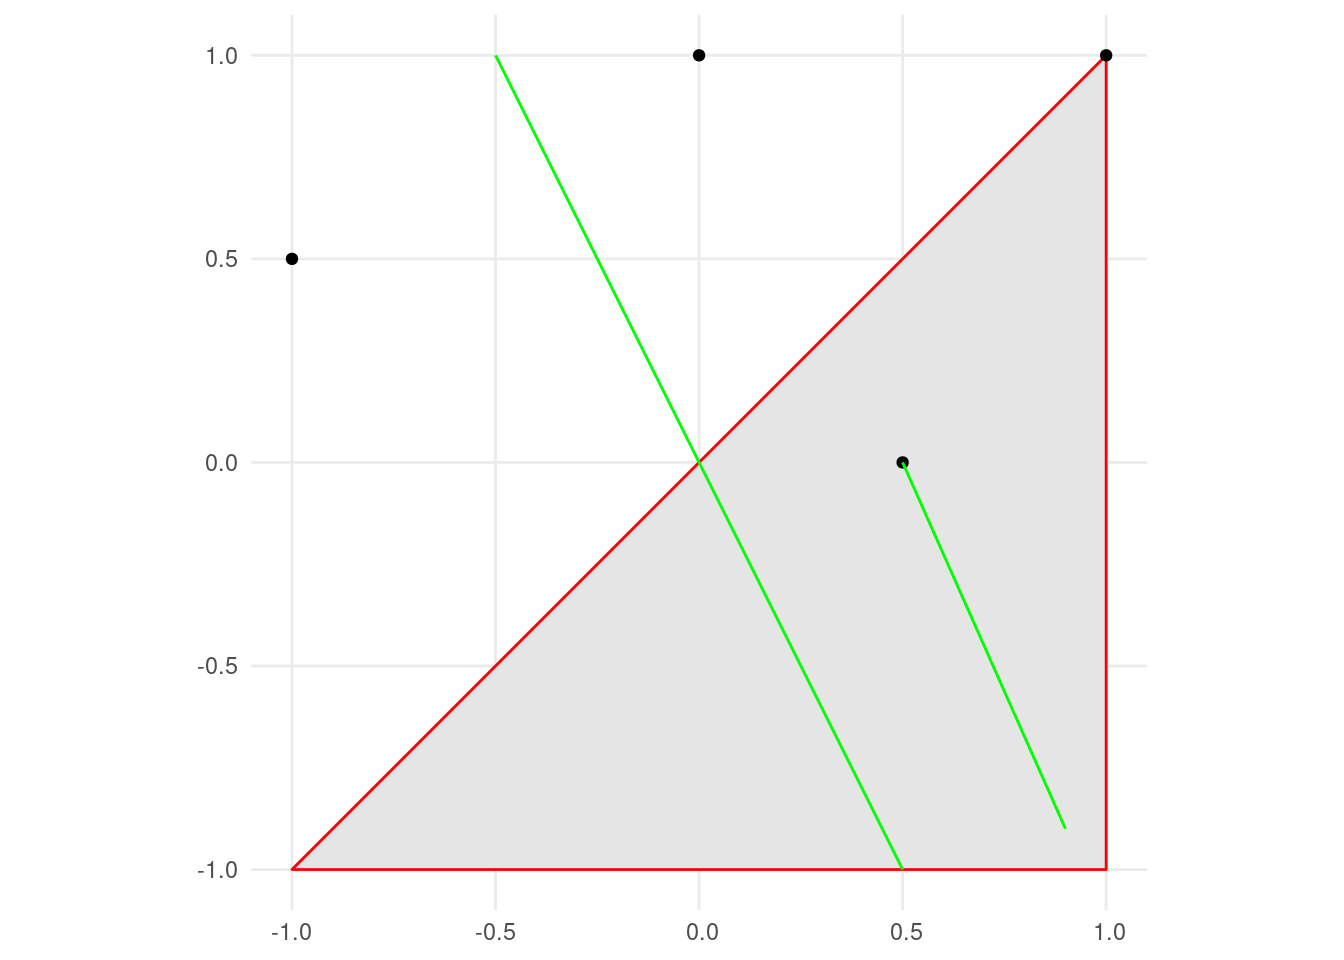
\includegraphics{support_m7_files/figure-latex/unnamed-chunk-34-1.pdf}

A partir de ces objets, on peut se poser les questions suivantes :

\begin{itemize}
\item
  Quels sont les points de \texttt{p} contenus dans le triangle \texttt{a} ?
\item
  Quels sont les points de \texttt{p} qui ne sont pas contenus dans le triangle \texttt{a} ?
\item
  Quels sont les points de \texttt{p} qui touchent le triangle \texttt{a} ?
\item
  Quelles sont les lignes de \texttt{l} contenues dans \texttt{a} ?
\end{itemize}

Les prédicats spatiaux vont nous permettre de répondre à ces questions. \texttt{sf} contient une liste de fonctions qui permettent chacune de répondre à l'une ou l'autre de ces questions.

\texttt{st\_intersects()} permet de répondre à la première question, à savoir quels points de \texttt{p} sont dans \texttt{a}.

\begin{Shaded}
\begin{Highlighting}[]
\FunctionTok{st\_intersects}\NormalTok{(p, a)}
\end{Highlighting}
\end{Shaded}

\begin{verbatim}
Sparse geometry binary predicate list of length 4, where the predicate
was `intersects'
 1: 1
 2: 1
 3: (empty)
 4: (empty)
\end{verbatim}

L'opposé de \texttt{st\_intersects()} est \texttt{st\_disjoint()} : \texttt{st\_disjoint(x,y)} renvoie \texttt{TRUE} pour les objets de \texttt{x} non reliés à \texttt{y}.

\begin{Shaded}
\begin{Highlighting}[]
\FunctionTok{st\_disjoint}\NormalTok{(p, a)}
\end{Highlighting}
\end{Shaded}

\begin{verbatim}
Sparse geometry binary predicate list of length 4, where the predicate
was `disjoint'
 1: (empty)
 2: (empty)
 3: 1
 4: 1
\end{verbatim}

Le résultat de cette opération est une liste. Par défaut, la fonction \texttt{st\_intersect()} renvoie une \emph{matrice creuse}\footnote{\url{https://fr.wikipedia.org/wiki/Matrice_creuse}}. Cette structure permet d'économiser de la mémoire en n'enregistrant que les relations qui existent. Sur une opération de ce type, le gain est peu évident, mais quand on travail sur des objets plus complexes, le gain est appréciable.

Si on souhaite mieux utiliser cette information, on peut vouloir privilégier la \emph{matrice dense}, qui renvoie une matrice de booléen pour chaque relation possible.

Pour cela on peut utiliser l'option \texttt{sparse=F}.

\begin{Shaded}
\begin{Highlighting}[]
\FunctionTok{st\_intersects}\NormalTok{(p, a, }\AttributeTok{sparse =}\NormalTok{ F)}
\end{Highlighting}
\end{Shaded}

\begin{verbatim}
      [,1]
[1,]  TRUE
[2,]  TRUE
[3,] FALSE
[4,] FALSE
\end{verbatim}

\texttt{st\_within()} est une variante de \texttt{st\_intersect()} qui ne renvoie \texttt{TRUE} que pour les points \emph{à l'intérieur} du polygone.

\begin{Shaded}
\begin{Highlighting}[]
\FunctionTok{st\_within}\NormalTok{(p, a, }\AttributeTok{sparse =}\NormalTok{ F)}
\end{Highlighting}
\end{Shaded}

\begin{verbatim}
      [,1]
[1,]  TRUE
[2,] FALSE
[3,] FALSE
[4,] FALSE
\end{verbatim}

Une variante de \texttt{st\_within()} permet d'ajouter un critère de distance pour intégrer des points \emph{presque} dans le polygone, \texttt{st\_is\_within\_distance()}.

\begin{Shaded}
\begin{Highlighting}[]
\FunctionTok{st\_is\_within\_distance}\NormalTok{(p, a, }\AttributeTok{dist =} \FloatTok{0.8}\NormalTok{)}
\end{Highlighting}
\end{Shaded}

\begin{verbatim}
Sparse geometry binary predicate list of length 4, where the predicate
was `is_within_distance'
 1: 1
 2: 1
 3: (empty)
 4: 1
\end{verbatim}

\texttt{st\_touches()} permet de récupérer les points qui \emph{touchent} le polygone sans sans être à l'intérieur du polygone.

\begin{Shaded}
\begin{Highlighting}[]
\FunctionTok{st\_touches}\NormalTok{(p, a, }\AttributeTok{sparse =}\NormalTok{ F)}
\end{Highlighting}
\end{Shaded}

\begin{verbatim}
      [,1]
[1,] FALSE
[2,]  TRUE
[3,] FALSE
[4,] FALSE
\end{verbatim}

\texttt{st\_contains(x,y)} est équivalent à \texttt{st\_within(y,x)}. Par exemple si nous voulons savoir lesquelles de nos lignes \texttt{l} sont contenues dans \texttt{a}.

\begin{Shaded}
\begin{Highlighting}[]
\FunctionTok{st\_contains}\NormalTok{(a, l, }\AttributeTok{sparse =}\NormalTok{ F)}
\end{Highlighting}
\end{Shaded}

\begin{verbatim}
      [,1] [,2]
[1,] FALSE TRUE
\end{verbatim}

Equivalent à :

\begin{Shaded}
\begin{Highlighting}[]
\FunctionTok{st\_within}\NormalTok{(l, a, }\AttributeTok{sparse =}\NormalTok{ F)}
\end{Highlighting}
\end{Shaded}

\begin{verbatim}
      [,1]
[1,] FALSE
[2,]  TRUE
\end{verbatim}

\texttt{st\_crosses()} renvoie TRUE si l'intersection des deux géométries est une géométrie de dimension n-1 ou n est le maximum des dimensions des deux objets et si l'intersection est à l'intérieur des deux objets.

\begin{Shaded}
\begin{Highlighting}[]
\FunctionTok{st\_crosses}\NormalTok{(l, a, }\AttributeTok{sparse =}\NormalTok{ F)}
\end{Highlighting}
\end{Shaded}

\begin{verbatim}
      [,1]
[1,]  TRUE
[2,] FALSE
\end{verbatim}

Il existent encore d'autres prédicats qu'on ne détaillera pas ici :

\begin{itemize}
\item
  \texttt{st\_covers()}
\item
  \texttt{st\_covered\_by()}
\item
  \texttt{st\_equals()} et \texttt{st\_equals\_exact()}
\item
  \texttt{st\_contains\_properly()}
\item
  \texttt{st\_overlaps()}
\end{itemize}

\hypertarget{exercices}{%
\subsection{Exercices}\label{exercices}}

\begin{itemize}
\tightlist
\item
  Créer un objet des points de p qui intersectent avec le polygone a
\end{itemize}

\hypertarget{les-jointures-spatiales}{%
\section{Les jointures spatiales}\label{les-jointures-spatiales}}

Les jointures \emph{attributaires} se basent sur un appariement sur une liste des variables présentes dans les deux tables.

Les jointures spatiales se basent sur un appariement sur un espace geographique commun.

\hypertarget{jointure-de-points-avec-des-polygones}{%
\subsection{Jointure de points avec des polygones}\label{jointure-de-points-avec-des-polygones}}

Ce cas est relativement simple, une jointure spatiale entre une liste de points et une liste de polygones va attribuer pour chaque point le polygone auquel il appartient.

On va utiliser ici le fichier sirene du département de Loire Atlantique géocodé par Christian Quest\footnote{\url{http://data.cquest.org/geo_sirene/}}.
Prenons les entreprises de production de sel sur ce département et regardons dans quelle partie du territoire elles se trouvent.

\begin{Shaded}
\begin{Highlighting}[]
\FunctionTok{load}\NormalTok{(}\StringTok{"extdata/sirene.RData"}\NormalTok{)}
\end{Highlighting}
\end{Shaded}

\begin{Shaded}
\begin{Highlighting}[]
\NormalTok{sirene44\_sel }\OtherTok{\textless{}{-}}\NormalTok{ sirene44 }\SpecialCharTok{\%\textgreater{}\%}
  \FunctionTok{filter}\NormalTok{(APET700 }\SpecialCharTok{==} \StringTok{"0893Z"}\NormalTok{)}

\FunctionTok{mapview}\NormalTok{(}\FunctionTok{list}\NormalTok{(departement\_44, epci\_d44, sirene44\_sel), }\AttributeTok{zcol =} \FunctionTok{list}\NormalTok{(}\StringTok{"NOM\_DEP"}\NormalTok{, }\StringTok{"NOM\_EPCI"}\NormalTok{, }\StringTok{"NOMEN\_LONG"}\NormalTok{), }\AttributeTok{legend =}\NormalTok{ F)}
\end{Highlighting}
\end{Shaded}

\includegraphics{support_m7_files/figure-latex/unnamed-chunk-45-1.pdf}

Nous allons réaliser une jointure spatiale pour récupérer le code sirene de l'EPCI où se trouve chaque entreprise.

\begin{Shaded}
\begin{Highlighting}[]
\NormalTok{sirene44\_sel\_avec\_code\_epci }\OtherTok{\textless{}{-}}\NormalTok{ sirene44\_sel }\SpecialCharTok{\%\textgreater{}\%}
  \FunctionTok{st\_join}\NormalTok{(epci\_geo)}
\end{Highlighting}
\end{Shaded}

\begin{Shaded}
\begin{Highlighting}[]
\FunctionTok{mapview}\NormalTok{(}\FunctionTok{list}\NormalTok{(departement\_44, epci\_d44, sirene44\_sel\_avec\_code\_epci), }\AttributeTok{zcol =} \FunctionTok{list}\NormalTok{(}\StringTok{"NOM\_DEP"}\NormalTok{, }\StringTok{"NOM\_EPCI"}\NormalTok{, }\StringTok{"NOM\_EPCI"}\NormalTok{), }\AttributeTok{legend =}\NormalTok{ F)}
\end{Highlighting}
\end{Shaded}

\includegraphics{support_m7_files/figure-latex/unnamed-chunk-47-1.pdf}

\begin{rmdnote}
Une jointure entre deux couches de données géographique demande à ce que celles-ci partagent la même projection.
\end{rmdnote}

\hypertarget{jointure-de-polygones-avec-des-polygones}{%
\subsection{Jointure de polygones avec des polygones}\label{jointure-de-polygones-avec-des-polygones}}

A la différence des appariements entre points et polygones, la jointure spatiales entre deux couches de polygones nécessite quelques critères complémentaires : souhaite-t-on joindre deux polygones dès qu'ils s'intersectent ? Souhaite-t-on joindre à un polygone de la première couche à celui de la deuxième avec lequel il partage le plus de surface en commun ?

Par exemple, imaginons que nous voulions joindre notre couche des epci avec celle des départements, souhaite-t-on que l'EPCI de Redon se retrouve apparié avec tous les départements dans lesquels il se retrouve, ou seulement le département dans lequel il est principalement situé ?

\begin{Shaded}
\begin{Highlighting}[]
\NormalTok{epci\_d44\_avec\_departement }\OtherTok{\textless{}{-}}\NormalTok{ epci\_d44 }\SpecialCharTok{\%\textgreater{}\%}
  \FunctionTok{st\_join}\NormalTok{(departements\_geo }\SpecialCharTok{\%\textgreater{}\%} \FunctionTok{st\_buffer}\NormalTok{(}\AttributeTok{dist =} \SpecialCharTok{{-}}\DecValTok{1000}\NormalTok{))}

\NormalTok{epci\_d44\_avec\_departement }\SpecialCharTok{\%\textgreater{}\%}
  \FunctionTok{select}\NormalTok{(NOM\_EPCI, NOM\_DEP) }\SpecialCharTok{\%\textgreater{}\%}
  \FunctionTok{group\_by}\NormalTok{(NOM\_EPCI) }\SpecialCharTok{\%\textgreater{}\%}
  \FunctionTok{tally}\NormalTok{() }\SpecialCharTok{\%\textgreater{}\%}
  \FunctionTok{arrange}\NormalTok{(}\SpecialCharTok{{-}}\NormalTok{n)}
\end{Highlighting}
\end{Shaded}

\begin{verbatim}
Simple feature collection with 17 features and 2 fields
Geometry type: MULTIPOLYGON
Dimension:     XY
Bounding box:  xmin: 276225 ymin: 6649968 xmax: 406328 ymax: 6763850
Projected CRS: RGF93 / Lambert-93
# A tibble: 17 x 3
   NOM_EPCI                        n                                    geometry
   <fct>                       <int>                          <MULTIPOLYGON [m]>
 1 CA Redon Agglomération          3 (((306620 6741720, 306267 6741867, 306062 ~
 2 CA de la Presqu'île de Gué~     2 (((276339 6716135, 276289 6716140, 276269 ~
 3 CC du Pays d'Ancenis            2 (((371339 6714790, 371319 6714805, 371304 ~
 4 CA Clisson Sèvre et Maine ~     1 (((363286 6675340, 363132 6675446, 363108 ~
 5 CA de la Région Nazairienn~     1 (((302551 6716906, 302541 6716916, 302491 ~
 6 CA Pornic Agglo Pays de Re~     1 (((308476 6686309, 308598 6686453, 308658 ~
 7 CC Châteaubriant-Derval         1 (((352474 6745979, 352438 6746143, 352414 ~
 8 CC d'Erdre et Gesvres           1 (((344433 6712377, 344438 6712392, 344469 ~
 9 CC de Grand Lieu                1 (((350722 6678570, 350738 6678630, 350788 ~
10 CC de la Région de Blain        1 (((347300 6718329, 347160 6718370, 347100 ~
11 CC de Nozay                     1 (((348972 6729772, 348993 6729802, 349018 ~
12 CC du Pays de Pontchâteau ~     1 (((316649 6727168, 316675 6727223, 316680 ~
13 CC du Sud-Estuaire              1 (((312929 6700671, 313386 6700816, 313902 ~
14 CC Estuaire et Sillon           1 (((321943 6705416, 321938 6705506, 321910 ~
15 CC Sèvre et Loire               1 (((369368 6686432, 369283 6686483, 369089 ~
16 CC Sud Retz Atlantique          1 (((336398 6673676, 336413 6673726, 336494 ~
17 Nantes Métropole                1 (((353637 6695899, 353628 6696029, 353604 ~
\end{verbatim}

Une jointure classique va donc rattacher 3 epci à plus de 1 département.

Avec l'option \texttt{largest\ =\ TRUE} la jointure va attribuer aux epci le département avec lequel il partage le plus de surface.
On voit ici que tout les epci adhérents à la Loire Atlantique se retrouvent alors rattachés à la Loire Atlantique.

\begin{Shaded}
\begin{Highlighting}[]
\NormalTok{epci\_d44\_avec\_departement }\OtherTok{\textless{}{-}}\NormalTok{ epci\_d44 }\SpecialCharTok{\%\textgreater{}\%}
  \FunctionTok{st\_join}\NormalTok{(departements\_geo }\SpecialCharTok{\%\textgreater{}\%} \FunctionTok{st\_buffer}\NormalTok{(}\AttributeTok{dist =} \SpecialCharTok{{-}}\DecValTok{1000}\NormalTok{), }\AttributeTok{largest =} \ConstantTok{TRUE}\NormalTok{)}

\FunctionTok{mapview}\NormalTok{(}\FunctionTok{list}\NormalTok{(departement\_44, epci\_d44, sirene44\_sel\_avec\_code\_epci), }\AttributeTok{zcol =} \FunctionTok{list}\NormalTok{(}\StringTok{"NOM\_DEP"}\NormalTok{, }\StringTok{"NOM\_EPCI"}\NormalTok{, }\StringTok{"NOM\_EPCI"}\NormalTok{), }
        \AttributeTok{legend =} \ConstantTok{FALSE}\NormalTok{)}
\end{Highlighting}
\end{Shaded}

\includegraphics{support_m7_files/figure-latex/unnamed-chunk-50-1.pdf}

\hypertarget{exercice}{%
\subsection{Exercice}\label{exercice}}

Le but de cet exercice va être d'exploiter les données \emph{DVF} sur les transactions immobilières dans l'ancien et la carte des quartiers de Nantes pour obtenir un prix moyen des transactions par quartier.
On va utiliser pour DVF l'API mise en place par Christian Quest.

\begin{itemize}
\item
  Données DVF : \url{http://api.cquest.org/dvf}
\item
  Contour des quartiers de Nantes : \url{https://data.nantesmetropole.fr/explore/dataset/244400404_quartiers-nantes/information/?disjunctive.nom}
\end{itemize}

On veut produire les infos suivantes par quartier et année :

\begin{itemize}
\tightlist
\item
  Volume de ventes
\item
  Pourcentage de maisons dans les ventes
\item
  Prix moyen au m2 par type de bien
\end{itemize}

\hypertarget{les-calculs-de-distance}{%
\section{Les calculs de distance}\label{les-calculs-de-distance}}

\hypertarget{matrice-de-distances}{%
\subsection{Matrice de distances}\label{matrice-de-distances}}

Contrairement aux opérations précédentes qui sont binaires, les opérations de distance sont continues.

Les distances se calculent avec la fonction \texttt{st\_distance()}.

\begin{Shaded}
\begin{Highlighting}[]
\NormalTok{centres\_departements\_pdl }\OtherTok{\textless{}{-}} \FunctionTok{st\_centroid}\NormalTok{(departements\_geo) }\SpecialCharTok{\%\textgreater{}\%}
  \FunctionTok{filter}\NormalTok{(INSEE\_REG }\SpecialCharTok{==} \StringTok{"52"}\NormalTok{)}

\FunctionTok{st\_distance}\NormalTok{(centres\_departements\_pdl)}
\end{Highlighting}
\end{Shaded}

\begin{verbatim}
Units: [m]
          [,1]     [,2]      [,3]      [,4]      [,5]
[1,]      0.00 84564.06 115956.62 159032.47  81705.88
[2,]  84564.06     0.00  84434.09  89195.57  97175.56
[3,] 115956.62 84434.09      0.00  67722.46 170458.60
[4,] 159032.47 89195.57  67722.46      0.00 186168.94
[5,]  81705.88 97175.56 170458.60 186168.94      0.00
\end{verbatim}

Trois choses à noter sur le résultat :

\begin{itemize}
\item
  \texttt{st\_distance()} retourne une \emph{matrice}\ldots{}
\item
  \ldots{} contenant toute les distances calculables 2 à 2\ldots{}
\item
  \ldots et qui a un paramètre \texttt{Units} nous donnant l'unité de mesure des distances calculées.
\end{itemize}

Ici on calcule notre matrice sur un seul objet. Vous pouvez calculer des distances entre deux objets \texttt{x} et \texttt{y} de classe \texttt{sf}. Dans ce cas il fera le calcul des distances pour toutes les combinaisons possibles d'objets de \texttt{x} et de \texttt{y}. Une option de \texttt{st\_distance()} vous permet de limiter le résultat aux calculs 2 à 2 : \texttt{by\_element\ =\ T}. Dans ce cas le résultat est un vecteur.

\hypertarget{identification-du-plus-proche-voisin}{%
\subsection{Identification du plus proche voisin}\label{identification-du-plus-proche-voisin}}

Un besoin fréquent en traitement géomatique est d'identifier l'objet le plus proche d'un autre.
La fonction qui permet cela est \texttt{st\_nearest\_feature()}.

Prenons l'ensemble des départements français, et trouvons celui de la région le plus proche. On va utiliser les centroïdes pour alléger le calcul.

\begin{Shaded}
\begin{Highlighting}[]
\NormalTok{index\_dep\_pdl }\OtherTok{\textless{}{-}} \FunctionTok{st\_nearest\_feature}\NormalTok{(}
\NormalTok{  departements\_geo,}
\NormalTok{  centres\_departements\_pdl}
\NormalTok{)}
\end{Highlighting}
\end{Shaded}

\texttt{st\_nearest\_feature()} renvoie un vecteur d'index en résultat.

Pour visualiser cet index, vous pouvez utiliser ensuite la fonction \texttt{st\_nearest\_point()} qui va permettre de faire un lien entre les départements et le département ligérien le plus proche.

\texttt{st\_nearest\_point()} permet en effet de renvoyer pour deux géométries la ligne rejoignant les 2 points les plus proches.

\begin{Shaded}
\begin{Highlighting}[]
\NormalTok{liens }\OtherTok{\textless{}{-}} \FunctionTok{st\_nearest\_points}\NormalTok{(departements\_geo,}
\NormalTok{  centres\_departements\_pdl[index\_dep\_pdl, ],}
  \AttributeTok{pairwise =} \ConstantTok{TRUE}
\NormalTok{)}

\FunctionTok{ggplot}\NormalTok{() }\SpecialCharTok{+}
  \FunctionTok{geom\_sf}\NormalTok{(}\AttributeTok{data =}\NormalTok{ departements\_geo) }\SpecialCharTok{+}
  \FunctionTok{geom\_sf}\NormalTok{(}\AttributeTok{data =}\NormalTok{ liens)}
\end{Highlighting}
\end{Shaded}

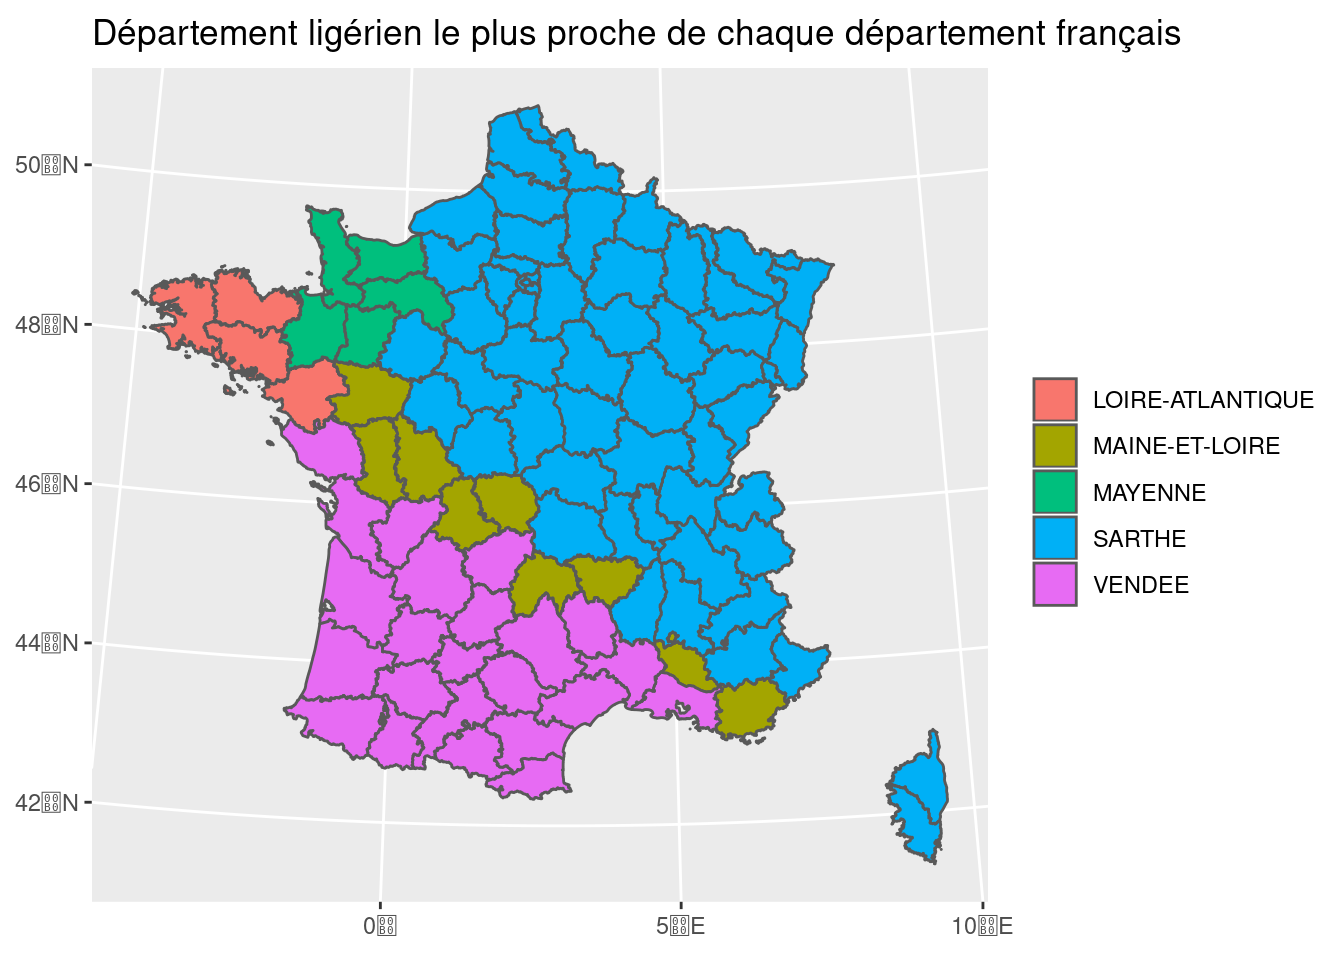
\includegraphics{support_m7_files/figure-latex/unnamed-chunk-53-1.pdf}

On peut utiliser aussi \texttt{st\_nearest\_feature()} comme un mode de jointure des données.

\begin{Shaded}
\begin{Highlighting}[]
\NormalTok{departements\_join }\OtherTok{\textless{}{-}} \FunctionTok{st\_join}\NormalTok{(departements\_geo,}
\NormalTok{  centres\_departements\_pdl,}
  \AttributeTok{join =}\NormalTok{ st\_nearest\_feature}
\NormalTok{)}

\FunctionTok{ggplot}\NormalTok{() }\SpecialCharTok{+}
  \FunctionTok{geom\_sf}\NormalTok{(}\AttributeTok{data =}\NormalTok{ departements\_join, }\FunctionTok{aes}\NormalTok{(}\AttributeTok{fill =}\NormalTok{ NOM\_DEP.y)) }\SpecialCharTok{+}
  \FunctionTok{labs}\NormalTok{(}
    \AttributeTok{title =} \StringTok{"Département ligérien le plus proche de chaque département français"}\NormalTok{,}
    \AttributeTok{fill =} \ConstantTok{NULL}
\NormalTok{  )}
\end{Highlighting}
\end{Shaded}

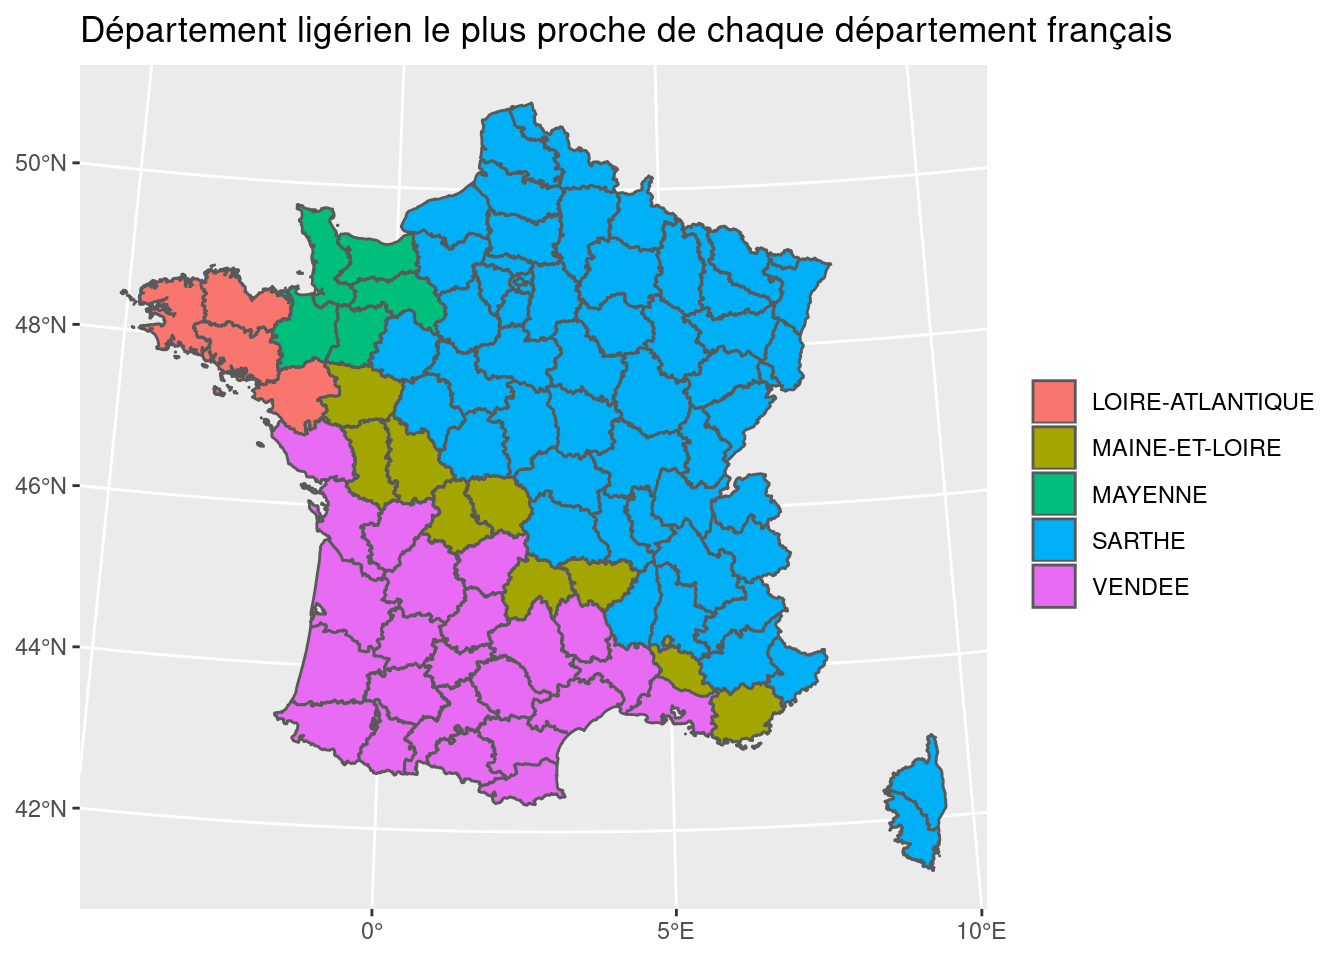
\includegraphics{support_m7_files/figure-latex/unnamed-chunk-54-1.pdf}

\hypertarget{les-opuxe9rations-guxe9omuxe9triques}{%
\chapter{Les opérations géométriques}\label{les-opuxe9rations-guxe9omuxe9triques}}

Nous allons voir dans ce chapitre comment opérer des opérations géométriques sur nos vecteurs.

Dans ce chapitre, nous allons utiliser les packages suivants.

\begin{Shaded}
\begin{Highlighting}[]
\FunctionTok{library}\NormalTok{(sf)}
\FunctionTok{library}\NormalTok{(tidyverse)}
\FunctionTok{library}\NormalTok{(mapview)}
\FunctionTok{library}\NormalTok{(ggplot2)}
\FunctionTok{library}\NormalTok{(rmapshaper)}
\FunctionTok{library}\NormalTok{(patchwork)}
\end{Highlighting}
\end{Shaded}

On distingue deux types d'opérations : les opérations unaires et binaires.

\hypertarget{opuxe9rations-unaires}{%
\section{Opérations unaires}\label{opuxe9rations-unaires}}

\hypertarget{simplification}{%
\subsection{Simplification}\label{simplification}}

La simplification revient comme son nom l'indique à simplifier une couche vectorielle. Le cas d'usage d'un tel procédé peut être un changement d'échelle et plus généralement le besoin de réduire la taille de stockage de notre objet (par exemple pour une publication ou une carte interactive).

Le package \texttt{sf} contient une fonction \texttt{st\_simplify} qui implémente l'algorithme de Douglas-Peucker\footnote{Douglas, David H, and Thomas K Peucker. 1973. ``Algorithms for the Reduction of the Number of Points Required to Represent a Digitized Line or Its Caricature.'' Cartographica: The International Journal for Geographic Information and Geovisualization 10 (2): 112--22.} de GEOS.

La fonction utilise le paramètre \texttt{dTolerance} pour controler le niveau de simplification.

\begin{Shaded}
\begin{Highlighting}[]
\FunctionTok{load}\NormalTok{(}\StringTok{"extdata/admin\_express.RData"}\NormalTok{)}
\end{Highlighting}
\end{Shaded}

\begin{Shaded}
\begin{Highlighting}[]
\NormalTok{departement\_56 }\OtherTok{\textless{}{-}}\NormalTok{ departements\_geo }\SpecialCharTok{\%\textgreater{}\%}
  \FunctionTok{filter}\NormalTok{(INSEE\_DEP }\SpecialCharTok{==} \StringTok{"56"}\NormalTok{)}

\NormalTok{departement\_56\_simplifie }\OtherTok{\textless{}{-}}\NormalTok{ departement\_56 }\SpecialCharTok{\%\textgreater{}\%}
  \FunctionTok{st\_simplify}\NormalTok{(}\AttributeTok{dTolerance =} \DecValTok{900}\NormalTok{)}

\NormalTok{departement\_56\_super\_simplifie }\OtherTok{\textless{}{-}}\NormalTok{ departement\_56 }\SpecialCharTok{\%\textgreater{}\%}
  \FunctionTok{st\_simplify}\NormalTok{(}\AttributeTok{dTolerance =} \DecValTok{2000}\NormalTok{)}
\end{Highlighting}
\end{Shaded}

\begin{Shaded}
\begin{Highlighting}[]
\NormalTok{p1 }\OtherTok{\textless{}{-}} \FunctionTok{ggplot}\NormalTok{() }\SpecialCharTok{+} 
  \FunctionTok{geom\_sf}\NormalTok{(}\AttributeTok{data =}\NormalTok{ departement\_56) }\SpecialCharTok{+} 
  \FunctionTok{theme\_void}\NormalTok{() }\SpecialCharTok{+} 
  \FunctionTok{theme}\NormalTok{(}\AttributeTok{panel.grid =} \FunctionTok{element\_blank}\NormalTok{(), }\AttributeTok{panel.border =} \FunctionTok{element\_blank}\NormalTok{())}

\NormalTok{p2 }\OtherTok{\textless{}{-}} \FunctionTok{ggplot}\NormalTok{() }\SpecialCharTok{+} 
  \FunctionTok{geom\_sf}\NormalTok{(}\AttributeTok{data =}\NormalTok{ departement\_56\_simplifie) }\SpecialCharTok{+}
  \FunctionTok{theme\_void}\NormalTok{()}

\NormalTok{p3 }\OtherTok{\textless{}{-}} \FunctionTok{ggplot}\NormalTok{() }\SpecialCharTok{+} 
  \FunctionTok{geom\_sf}\NormalTok{(}\AttributeTok{data =}\NormalTok{ departement\_56\_super\_simplifie) }\SpecialCharTok{+} 
  \FunctionTok{theme\_void}\NormalTok{()}

\NormalTok{p1 }\SpecialCharTok{+}\NormalTok{ p2 }\SpecialCharTok{+}\NormalTok{ p3 }\SpecialCharTok{+} \FunctionTok{plot\_layout}\NormalTok{(}\AttributeTok{nrow =} \DecValTok{1}\NormalTok{)}
\end{Highlighting}
\end{Shaded}

\includegraphics{support_m7_files/figure-latex/unnamed-chunk-58-1.pdf}

On peut mesurer le gain réalisé par chaque opération.

\begin{itemize}
\item
  Une simplification avec un \texttt{dTolerance} de 900 permet d'économiser 91.2 \% du stockage.
\item
  Une simplification avec un \texttt{dTolerance} de 2000 permet d'économiser 92.2 \% du stockage.
\end{itemize}

\begin{Shaded}
\begin{Highlighting}[]
\FunctionTok{object.size}\NormalTok{(departement\_56)}
\end{Highlighting}
\end{Shaded}

\begin{verbatim}
451008 bytes
\end{verbatim}

\begin{Shaded}
\begin{Highlighting}[]
\FunctionTok{object.size}\NormalTok{(departement\_56\_simplifie)}
\end{Highlighting}
\end{Shaded}

\begin{verbatim}
39496 bytes
\end{verbatim}

\begin{Shaded}
\begin{Highlighting}[]
\FunctionTok{object.size}\NormalTok{(departement\_56\_super\_simplifie)}
\end{Highlighting}
\end{Shaded}

\begin{verbatim}
34976 bytes
\end{verbatim}

Le problème de l'algorithme Douglas-Peucker est qu'il simplifie les géométries objet par objet. Cela conduit à perdre la topologie, et à des trous ou des chevauchements. L'option \texttt{preserveTopology\ =\ T} de \texttt{st\_simplify()} doit permettre en théorie d'éviter ce problème, mais ne marche pas au delà d'un certain seuil.

Par exemple, prenons 2 départements autour du Morbihan.

\begin{Shaded}
\begin{Highlighting}[]
\NormalTok{departements\_35\_44\_56 }\OtherTok{\textless{}{-}}\NormalTok{ departements\_geo }\SpecialCharTok{\%\textgreater{}\%}
  \FunctionTok{filter}\NormalTok{(INSEE\_DEP }\SpecialCharTok{\%in\%} \FunctionTok{c}\NormalTok{(}\StringTok{"35"}\NormalTok{, }\StringTok{"44"}\NormalTok{, }\StringTok{"56"}\NormalTok{))}

\NormalTok{departements\_35\_44\_56\_super\_simplifie }\OtherTok{\textless{}{-}}\NormalTok{ departements\_35\_44\_56 }\SpecialCharTok{\%\textgreater{}\%}
  \FunctionTok{st\_simplify}\NormalTok{(}\AttributeTok{dTolerance =} \DecValTok{3000}\NormalTok{)}
\end{Highlighting}
\end{Shaded}

\begin{Shaded}
\begin{Highlighting}[]
\NormalTok{p1 }\OtherTok{\textless{}{-}} \FunctionTok{ggplot}\NormalTok{() }\SpecialCharTok{+} 
  \FunctionTok{geom\_sf}\NormalTok{(}\AttributeTok{data =}\NormalTok{ departements\_35\_44\_56) }\SpecialCharTok{+} 
  \FunctionTok{theme\_void}\NormalTok{() }\SpecialCharTok{+} 
  \FunctionTok{theme}\NormalTok{(}\AttributeTok{panel.grid =} \FunctionTok{element\_blank}\NormalTok{(), }\AttributeTok{panel.border =} \FunctionTok{element\_blank}\NormalTok{())}

\NormalTok{p3 }\OtherTok{\textless{}{-}} \FunctionTok{ggplot}\NormalTok{() }\SpecialCharTok{+} 
  \FunctionTok{geom\_sf}\NormalTok{(}\AttributeTok{data =}\NormalTok{ departements\_35\_44\_56\_super\_simplifie) }\SpecialCharTok{+} 
  \FunctionTok{theme\_void}\NormalTok{()}

\NormalTok{p1 }\SpecialCharTok{+}\NormalTok{ p3 }\SpecialCharTok{+} \FunctionTok{plot\_layout}\NormalTok{(}\AttributeTok{nrow =} \DecValTok{1}\NormalTok{)}
\end{Highlighting}
\end{Shaded}

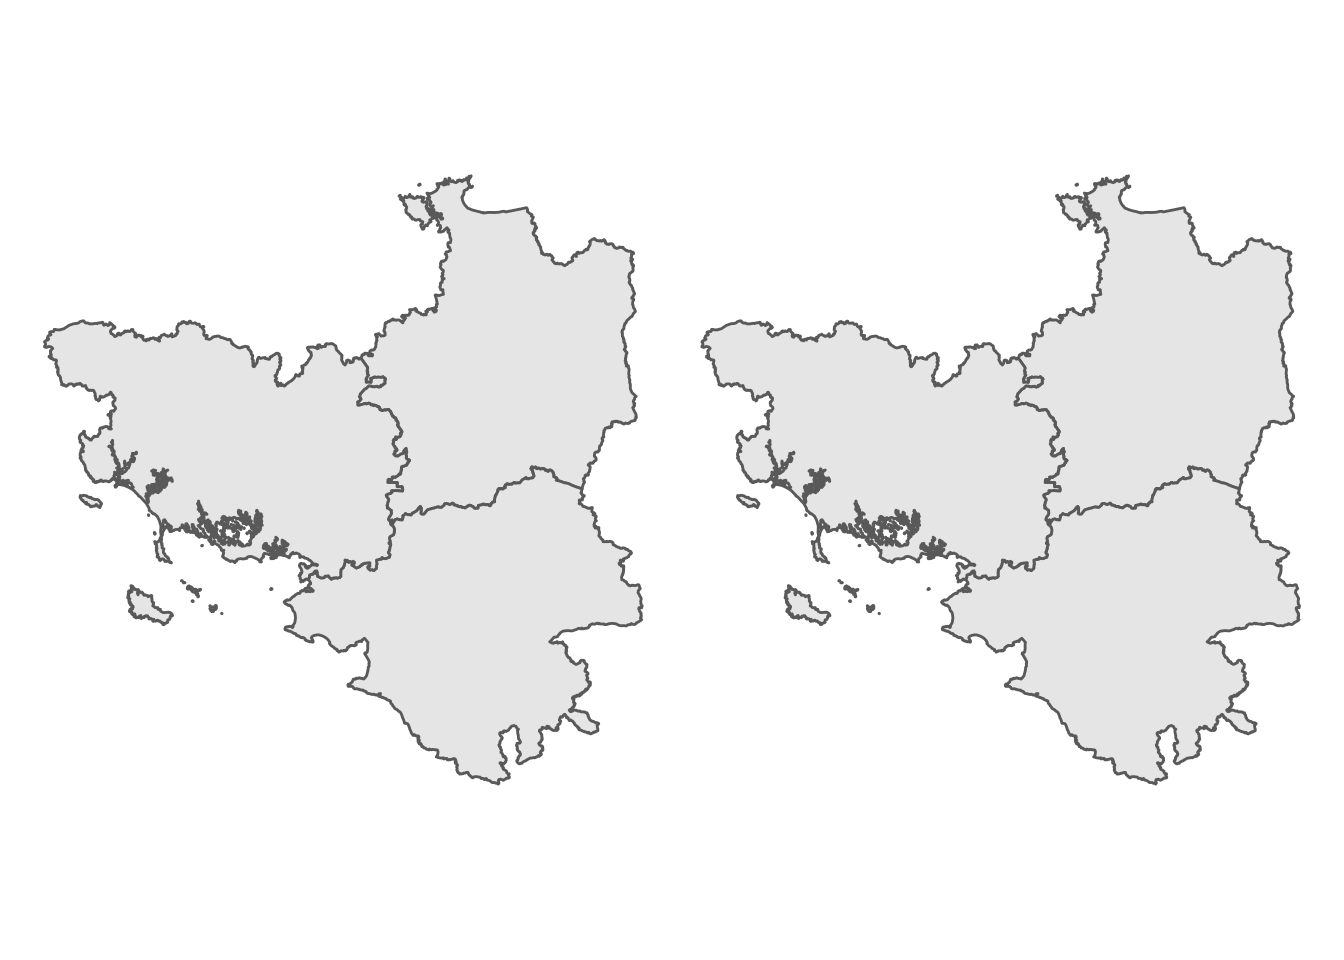
\includegraphics{support_m7_files/figure-latex/unnamed-chunk-61-1.pdf}

On constate clairement des trous à la frontière des 3 départements.

Un autre algorithme peut être utilisé qui n'a pas les mêmes limitations, l'algorithme de Visvalingam\footnote{Visvalingam, M., and J. D. Whyatt. 1993. ``Line Generalisation by Repeated Elimination of Points.'' The Cartographic Journal 30 (1): 46--51. \url{https://doi.org/10.1179/000870493786962263}.}.

Le package \texttt{rmapshaper} contient une fonction \texttt{ms\_simplify()} qui implémente cet algorithme.
Ce package est une interface vers Mapshaper\footnote{\url{https://mapshaper.org/}}, un site en ligne d'édition de données cartographiques.

\begin{Shaded}
\begin{Highlighting}[]
\NormalTok{departements\_35\_44\_56 }\OtherTok{\textless{}{-}}\NormalTok{ departements\_35\_44\_56 }\SpecialCharTok{\%\textgreater{}\%}
  \FunctionTok{mutate}\NormalTok{(}\AttributeTok{AREA =} \FunctionTok{as.numeric}\NormalTok{(AREA))}
\NormalTok{departements\_35\_44\_56\_ms\_simplifie }\OtherTok{\textless{}{-}} \FunctionTok{ms\_simplify}\NormalTok{(departements\_35\_44\_56, }\AttributeTok{method =} \StringTok{"vis"}\NormalTok{, }\AttributeTok{keep =} \FloatTok{0.01}\NormalTok{)}
\end{Highlighting}
\end{Shaded}

\begin{Shaded}
\begin{Highlighting}[]
\NormalTok{p1 }\OtherTok{\textless{}{-}} \FunctionTok{ggplot}\NormalTok{() }\SpecialCharTok{+} 
  \FunctionTok{geom\_sf}\NormalTok{(}\AttributeTok{data =}\NormalTok{ departements\_35\_44\_56) }\SpecialCharTok{+} 
  \FunctionTok{theme\_void}\NormalTok{() }\SpecialCharTok{+} 
  \FunctionTok{theme}\NormalTok{(}\AttributeTok{panel.grid =} \FunctionTok{element\_blank}\NormalTok{(), }\AttributeTok{panel.border =} \FunctionTok{element\_blank}\NormalTok{())}

\NormalTok{p3 }\OtherTok{\textless{}{-}} \FunctionTok{ggplot}\NormalTok{() }\SpecialCharTok{+} 
  \FunctionTok{geom\_sf}\NormalTok{(}\AttributeTok{data =}\NormalTok{ departements\_35\_44\_56\_ms\_simplifie) }\SpecialCharTok{+} 
  \FunctionTok{theme\_void}\NormalTok{()}

\NormalTok{p1 }\SpecialCharTok{+}\NormalTok{ p3 }\SpecialCharTok{+} \FunctionTok{plot\_layout}\NormalTok{(}\AttributeTok{nrow =} \DecValTok{1}\NormalTok{)}
\end{Highlighting}
\end{Shaded}

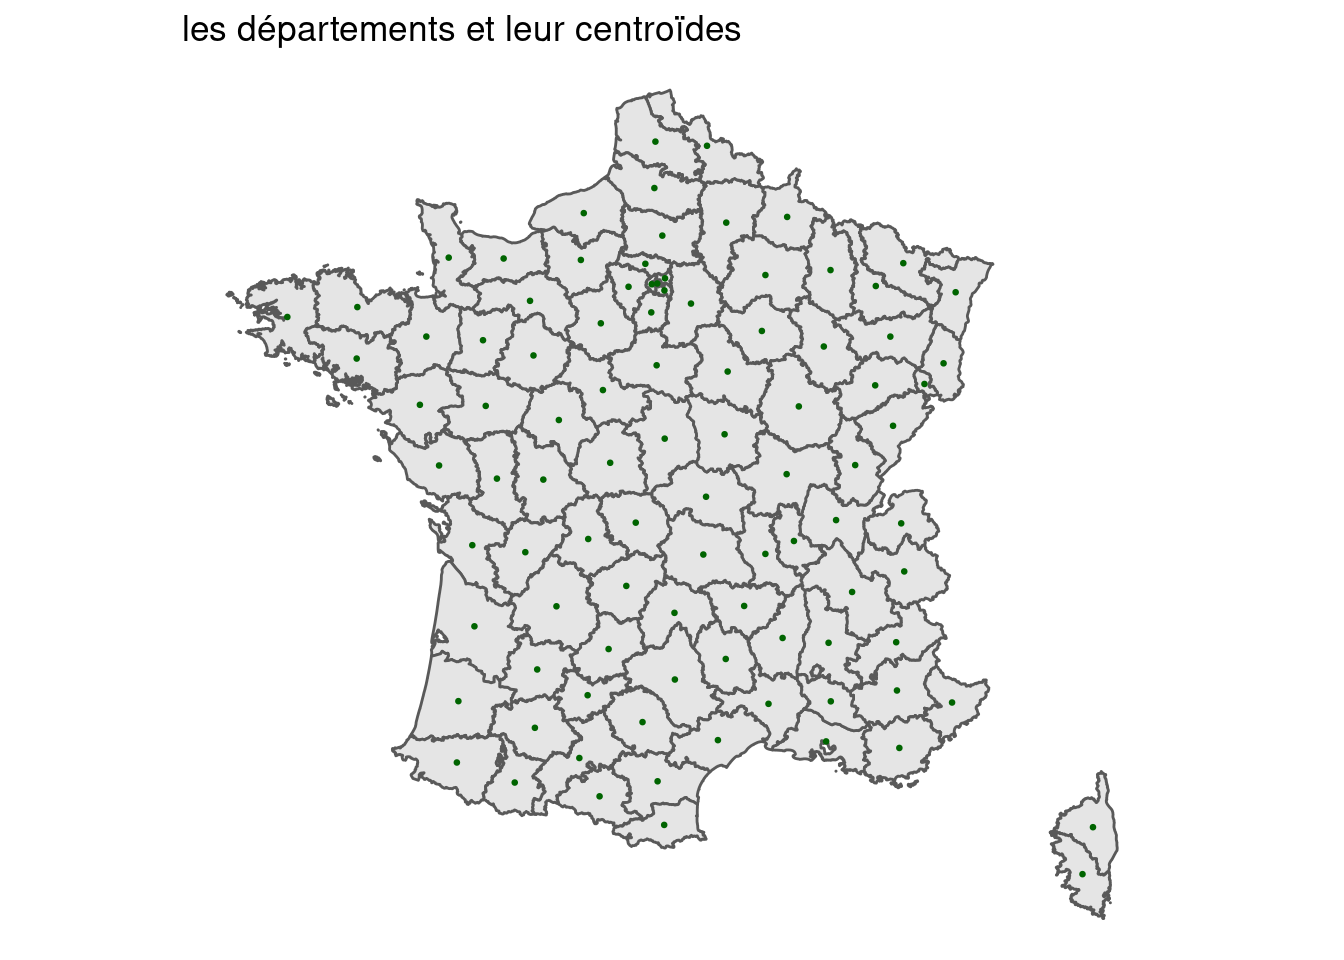
\includegraphics{support_m7_files/figure-latex/unnamed-chunk-63-1.pdf}

\hypertarget{centrouxefde}{%
\subsection{Centroïde}\label{centrouxefde}}

Le centroïde permet d'identifier le centre d'un objet géométrique. Il y a plusieurs façons de définir un centroïde. La plus usuelle est le centroïde géographique, qui peut être défini comme le point d'équilibre d'un objet (celui en dessous duquel votre doigt peut faire tenir en équilibre cet objet).
La fonction permettant de définir un centroïde dans \texttt{sf} est \texttt{st\_centroid()}.

\begin{Shaded}
\begin{Highlighting}[]
\NormalTok{centres\_departements }\OtherTok{\textless{}{-}} \FunctionTok{st\_centroid}\NormalTok{(departements\_geo)}
\end{Highlighting}
\end{Shaded}

\begin{Shaded}
\begin{Highlighting}[]
\FunctionTok{ggplot}\NormalTok{() }\SpecialCharTok{+}
  \FunctionTok{geom\_sf}\NormalTok{(}\AttributeTok{data =}\NormalTok{ departements\_geo) }\SpecialCharTok{+}
  \FunctionTok{geom\_sf}\NormalTok{(}\AttributeTok{data =}\NormalTok{ centres\_departements, }\AttributeTok{color =} \StringTok{"dark green"}\NormalTok{, }\AttributeTok{size =}\NormalTok{ .}\DecValTok{5}\NormalTok{) }\SpecialCharTok{+}
  \FunctionTok{theme\_void}\NormalTok{() }\SpecialCharTok{+}
  \FunctionTok{theme}\NormalTok{(}\AttributeTok{panel.grid =} \FunctionTok{element\_blank}\NormalTok{(), }\AttributeTok{panel.border =} \FunctionTok{element\_blank}\NormalTok{()) }\SpecialCharTok{+}
  \FunctionTok{labs}\NormalTok{(}\AttributeTok{title =} \StringTok{"les départements et leur centroïdes"}\NormalTok{)}
\end{Highlighting}
\end{Shaded}

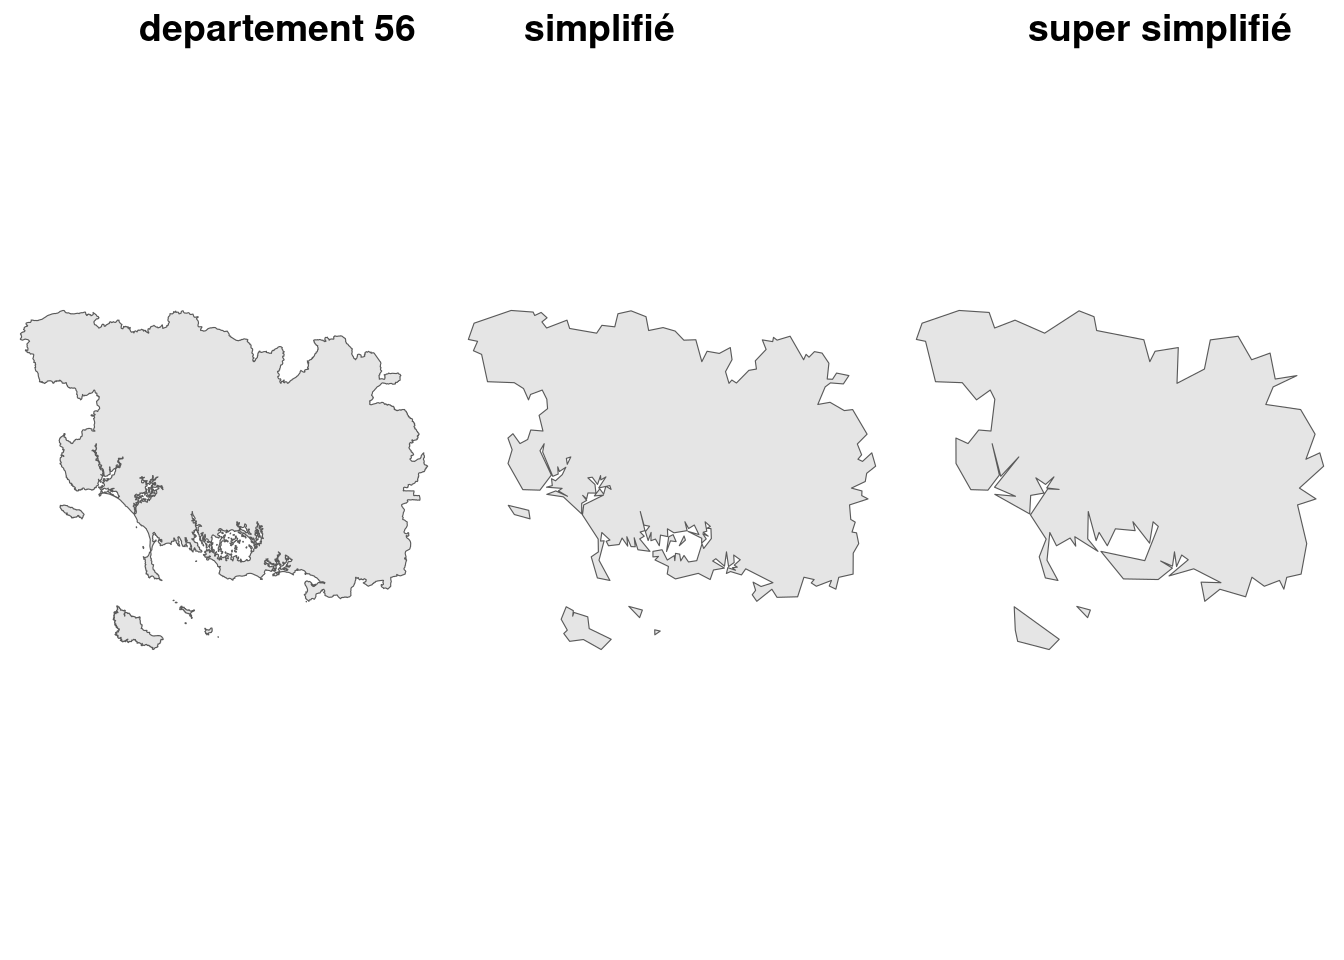
\includegraphics{support_m7_files/figure-latex/unnamed-chunk-65-1.pdf}

Parfois, le centroïde peut se placer en dehors de l'objet lui même. Par exemple pensez à un atoll.

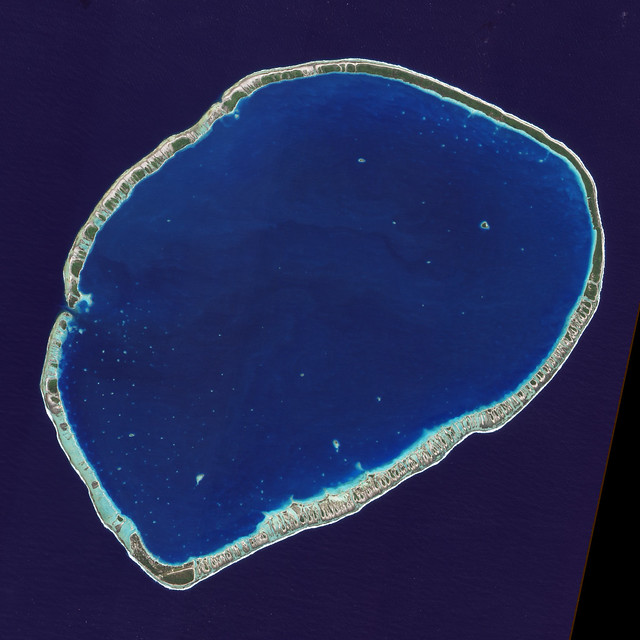
\includegraphics{pic/atoll.jpg}

Dans ce cas on peut utiliser \texttt{st\_point\_on\_surface()} qui garantit que le point est sur la surface de l'objet de départ.

\hypertarget{buffer}{%
\subsection{Buffer}\label{buffer}}

Comme déjà vu, à partir d'une couche de départ de type ponctuel, linéaire ou polygonal, le buffer va créer une nouvelle couche vectorielle. La géométrie de cette couche représente des objets surfaciques dont les frontières sont positionnées à une distance euclidienne, définie par l'utilisateur, des limites des objets vectoriels de la couche de départ.

\begin{Shaded}
\begin{Highlighting}[]
\NormalTok{departement\_44\_buffer }\OtherTok{\textless{}{-}}\NormalTok{ departement\_44 }\SpecialCharTok{\%\textgreater{}\%}
  \FunctionTok{st\_buffer}\NormalTok{(}\AttributeTok{dist =} \DecValTok{5000}\NormalTok{)}

\FunctionTok{mapview}\NormalTok{(}\FunctionTok{list}\NormalTok{(departement\_44\_buffer, departement\_44), }\AttributeTok{layer.name =} \FunctionTok{list}\NormalTok{(}\StringTok{"Loire{-}Atlantique avec un buffer de 5 km"}\NormalTok{, }\StringTok{"Loire{-}Atlantique"}\NormalTok{), }\AttributeTok{zcol =} \FunctionTok{list}\NormalTok{(}\StringTok{"NOM\_DEP"}\NormalTok{, }\StringTok{"NOM\_DEP"}\NormalTok{), }\AttributeTok{col.regions =} \FunctionTok{list}\NormalTok{(}\StringTok{"\#440154FF"}\NormalTok{, }\StringTok{"\#FDE725FF"}\NormalTok{), }\AttributeTok{legend =} \ConstantTok{FALSE}\NormalTok{)}
\end{Highlighting}
\end{Shaded}

\includegraphics{support_m7_files/figure-latex/unnamed-chunk-66-1.pdf}

\hypertarget{opuxe9rations-binaires}{%
\section{Opérations binaires}\label{opuxe9rations-binaires}}

\hypertarget{transformation-affine}{%
\subsection{Transformation affine}\label{transformation-affine}}

Les tranformations affines regrouppent les transformations qui préservent les lignes et le parallélisme. A l'inverse les angles et les tailles ne le sont pas forcément.

Les transformations affines intègrent notamment les translations, les rotations et les changements d'échelle.

Le package \texttt{sf} implémente ces transformations pour les objets de classe \texttt{sfg} et \texttt{sfc}.

\hypertarget{translation}{%
\subsubsection{Translation}\label{translation}}

\begin{Shaded}
\begin{Highlighting}[]
\NormalTok{departement\_44\_sfc }\OtherTok{\textless{}{-}} \FunctionTok{st\_geometry}\NormalTok{(departement\_44)}

\NormalTok{departement\_44\_sfc\_trans }\OtherTok{\textless{}{-}}\NormalTok{ departement\_44\_sfc }\SpecialCharTok{+} \FunctionTok{c}\NormalTok{(}\DecValTok{10000}\NormalTok{, }\DecValTok{10000}\NormalTok{)}

\NormalTok{departement\_44\_trans }\OtherTok{\textless{}{-}} \FunctionTok{st\_set\_geometry}\NormalTok{(departement\_44, departement\_44\_sfc\_trans)}

\FunctionTok{st\_crs}\NormalTok{(departement\_44\_trans) }\OtherTok{\textless{}{-}} \FunctionTok{st\_crs}\NormalTok{(departement\_44)}

\FunctionTok{mapview}\NormalTok{(}\FunctionTok{list}\NormalTok{(departement\_44\_trans, departement\_44), }\AttributeTok{layer.name =} \FunctionTok{list}\NormalTok{(}\StringTok{"Loire{-}Atlantique avec déplacement affine de 10 km vers le nord et 10 km vers le sud"}\NormalTok{, }\StringTok{"Loire{-}Atlantique"}\NormalTok{), }\AttributeTok{zcol =} \FunctionTok{list}\NormalTok{(}\StringTok{"NOM\_DEP"}\NormalTok{, }\StringTok{"NOM\_DEP"}\NormalTok{), }\AttributeTok{col.regions =} \FunctionTok{list}\NormalTok{(}\StringTok{"\#440154FF"}\NormalTok{, }\StringTok{"\#FDE725FF"}\NormalTok{), }\AttributeTok{legend =} \ConstantTok{FALSE}\NormalTok{)}
\end{Highlighting}
\end{Shaded}

\includegraphics{support_m7_files/figure-latex/unnamed-chunk-67-1.pdf}

\hypertarget{changement-duxe9chelle}{%
\subsubsection{Changement d'échelle}\label{changement-duxe9chelle}}

Dans l'exemple suivant on va réduire par deux la surface de chacun des epci du département.
Pour cela on va recentrer les epci pour que les coodonnées des centroids soient à l'origine avant de diviser par deux les cordonnées des contours et réappliquer la translation au centroid.

\begin{Shaded}
\begin{Highlighting}[]
\NormalTok{epci\_d44\_sfc }\OtherTok{\textless{}{-}} \FunctionTok{st\_geometry}\NormalTok{(epci\_d44)}

\NormalTok{epci\_d44\_centroid\_sfc }\OtherTok{\textless{}{-}} \FunctionTok{st\_centroid}\NormalTok{(epci\_d44\_sfc)}

\NormalTok{epci\_d44\_centroid\_sfc\_scale }\OtherTok{\textless{}{-}}\NormalTok{ (epci\_d44\_sfc }\SpecialCharTok{{-}}\NormalTok{ epci\_d44\_centroid\_sfc) }\SpecialCharTok{*} \FloatTok{0.5} \SpecialCharTok{+}\NormalTok{ epci\_d44\_centroid\_sfc}

\NormalTok{epci\_d44\_centroid\_scale }\OtherTok{\textless{}{-}} \FunctionTok{st\_set\_geometry}\NormalTok{(epci\_d44, epci\_d44\_centroid\_sfc\_scale)}

\FunctionTok{st\_crs}\NormalTok{(epci\_d44\_centroid\_scale) }\OtherTok{\textless{}{-}} \FunctionTok{st\_crs}\NormalTok{(epci\_d44)}


\FunctionTok{mapview}\NormalTok{(}\FunctionTok{list}\NormalTok{(epci\_d44, epci\_d44\_centroid\_scale), }\AttributeTok{layer.name =} \FunctionTok{list}\NormalTok{(}\StringTok{"Epci de Loire{-}Atlantique"}\NormalTok{, }\StringTok{"Epci de Loire{-}Atlantique avec surface divisées par deux"}\NormalTok{), }\AttributeTok{zcol =} \FunctionTok{list}\NormalTok{(}\StringTok{"NOM\_EPCI"}\NormalTok{, }\StringTok{"NOM\_EPCI"}\NormalTok{), }\AttributeTok{col.regions =} \FunctionTok{list}\NormalTok{(}\StringTok{"\#440154FF"}\NormalTok{, }\StringTok{"\#FDE725FF"}\NormalTok{), }\AttributeTok{legend =} \ConstantTok{FALSE}\NormalTok{)}
\end{Highlighting}
\end{Shaded}

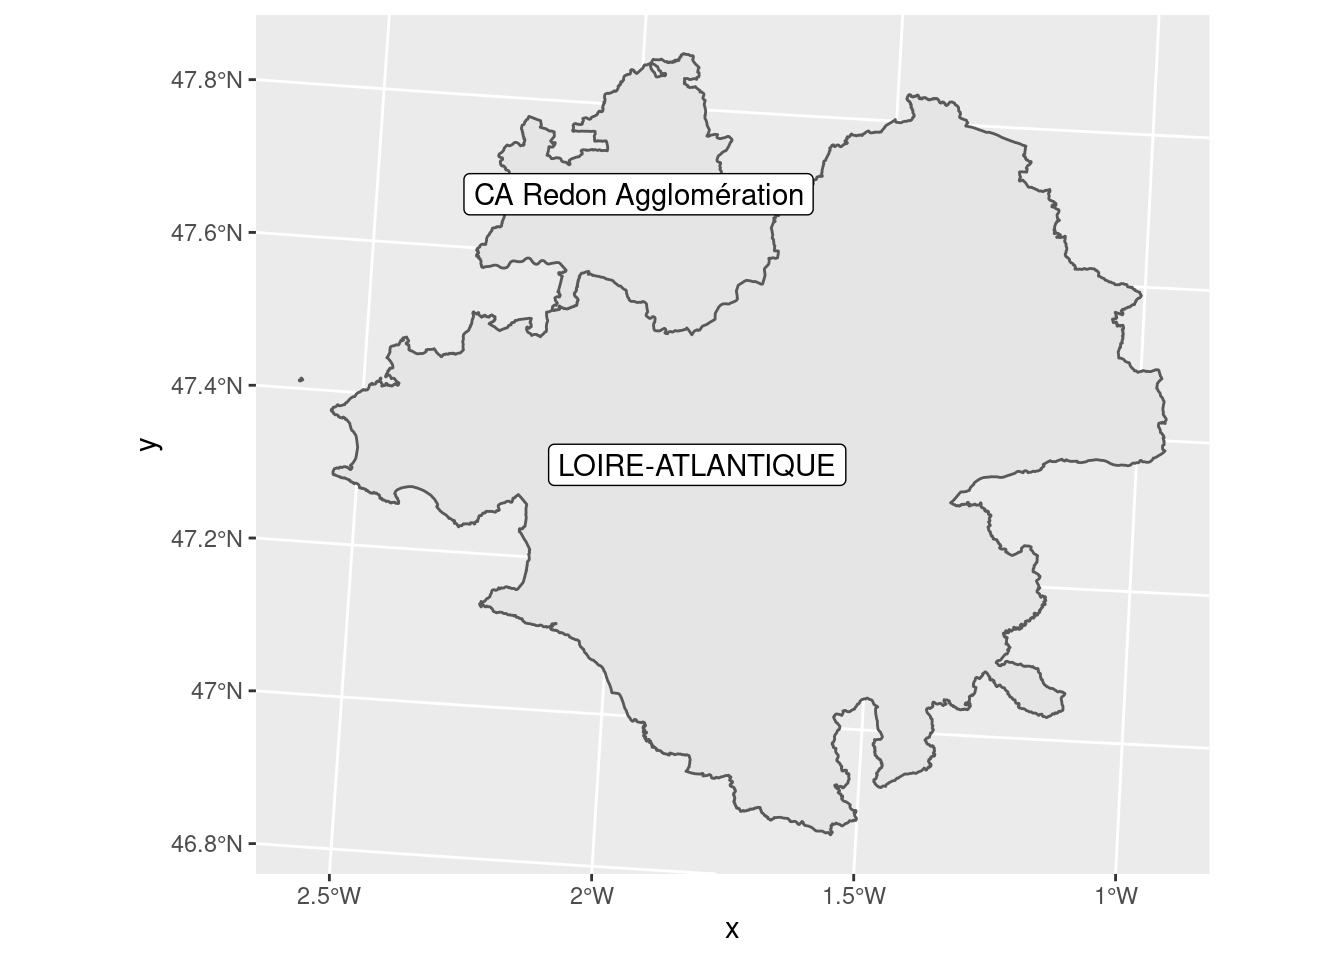
\includegraphics{support_m7_files/figure-latex/unnamed-chunk-68-1.pdf}

\hypertarget{duxe9coupage}{%
\subsection{Découpage}\label{duxe9coupage}}

Le découpage spatiale est une forme de filtre sur les géographies.

Le découpage peut seulement s'appliquer à des formes plus complexes que des points : (multi-)lignes, (multi-)polygones.

Nous allons illustrer le découpage à partir des epci à cheval sur plusieurs départements.

\begin{Shaded}
\begin{Highlighting}[]
\NormalTok{epci\_redon }\OtherTok{\textless{}{-}}\NormalTok{ epci\_d44 }\SpecialCharTok{\%\textgreater{}\%}
  \FunctionTok{filter}\NormalTok{(CODE\_EPCI }\SpecialCharTok{==} \StringTok{"243500741"}\NormalTok{)}
\end{Highlighting}
\end{Shaded}

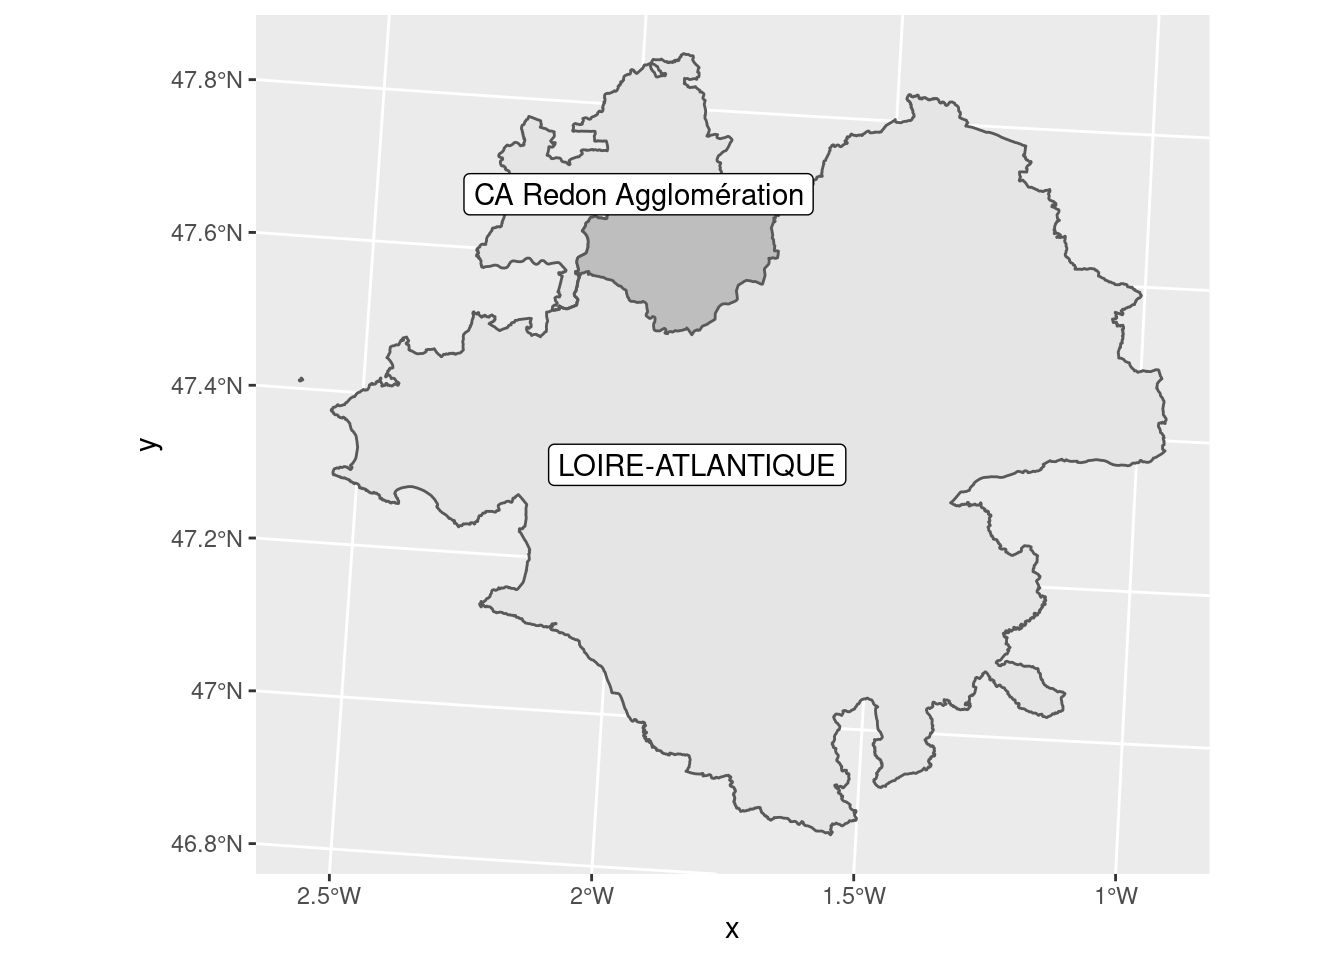
\includegraphics{support_m7_files/figure-latex/unnamed-chunk-70-1.pdf}

\texttt{st\_intersection()} permet de ne garder que la partie commune des deux géométries

\begin{Shaded}
\begin{Highlighting}[]
\NormalTok{redon\_et\_departement\_44 }\OtherTok{\textless{}{-}} \FunctionTok{st\_intersection}\NormalTok{(epci\_redon, departement\_44) }\SpecialCharTok{\%\textgreater{}\%}
  \FunctionTok{mutate}\NormalTok{(}\AttributeTok{NOM\_EPCI =} \StringTok{"Communes du 44 de la CA Redon Agglomération"}\NormalTok{)}
\end{Highlighting}
\end{Shaded}

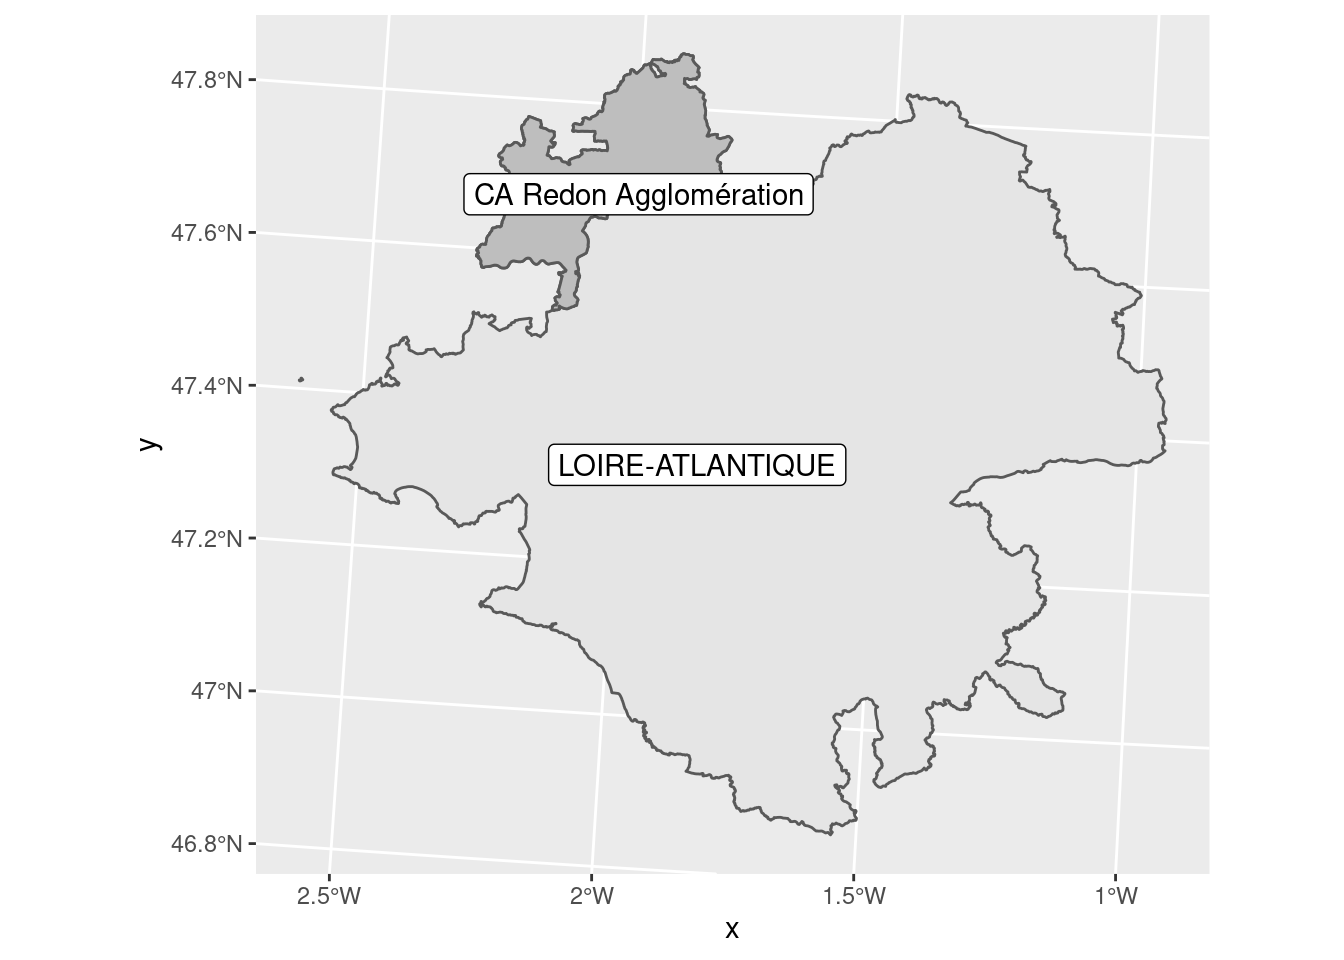
\includegraphics{support_m7_files/figure-latex/unnamed-chunk-72-1.pdf}

\texttt{st\_difference(x,y)} permet de ne garder que la partie de \texttt{x} non présente dans \texttt{y}

\begin{Shaded}
\begin{Highlighting}[]
\NormalTok{redon\_hors\_departement\_44 }\OtherTok{\textless{}{-}} \FunctionTok{st\_difference}\NormalTok{(epci\_redon, departement\_44) }\SpecialCharTok{\%\textgreater{}\%}
  \FunctionTok{mutate}\NormalTok{(}\AttributeTok{NOM\_EPCI =} \StringTok{"Communes du 44 et du CA Redon Agglomération hors communes en commun"}\NormalTok{)}
\end{Highlighting}
\end{Shaded}

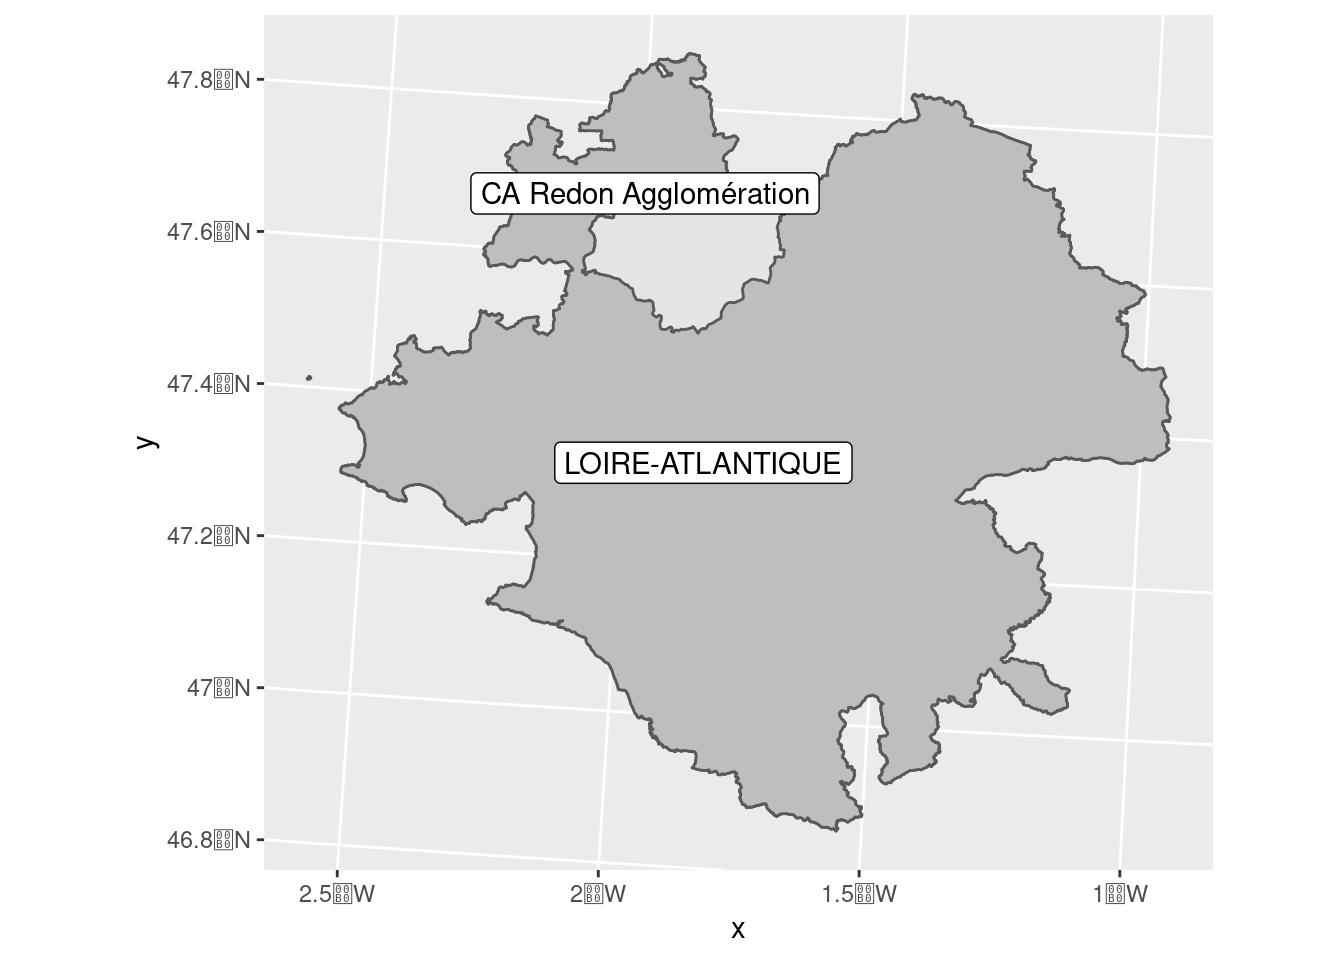
\includegraphics{support_m7_files/figure-latex/unnamed-chunk-74-1.pdf}

\texttt{st\_sym\_difference(x,y)} permet de ne garder que les partie de \texttt{x} et de \texttt{y} non communes.

\begin{Shaded}
\begin{Highlighting}[]
\NormalTok{redon\_et\_departement\_44\_sans\_partie\_communes }\OtherTok{\textless{}{-}} \FunctionTok{st\_sym\_difference}\NormalTok{(epci\_redon, departement\_44) }\SpecialCharTok{\%\textgreater{}\%}
  \FunctionTok{mutate}\NormalTok{(}\AttributeTok{NOM\_EPCI =} \StringTok{"Communes du 44 et du CA Redon Agglomération hors communes en commun"}\NormalTok{)}
\end{Highlighting}
\end{Shaded}

\includegraphics{support_m7_files/figure-latex/unnamed-chunk-76-1.pdf}

\hypertarget{union}{%
\subsection{Union}\label{union}}

Union permet de fusionner les géométries de plusieurs objets.
On va regarder comment reconsituer la carte des communes à partir de celle des départements

\begin{Shaded}
\begin{Highlighting}[]
\NormalTok{regions }\OtherTok{\textless{}{-}}\NormalTok{ departements\_geo }\SpecialCharTok{\%\textgreater{}\%}
  \FunctionTok{group\_by}\NormalTok{(INSEE\_REG) }\SpecialCharTok{\%\textgreater{}\%}
  \FunctionTok{summarise}\NormalTok{(}\AttributeTok{do\_union =}\NormalTok{ T)}
\end{Highlighting}
\end{Shaded}

\begin{Shaded}
\begin{Highlighting}[]
\FunctionTok{mapview}\NormalTok{(regions, }\AttributeTok{legend =}\NormalTok{ F)}
\end{Highlighting}
\end{Shaded}

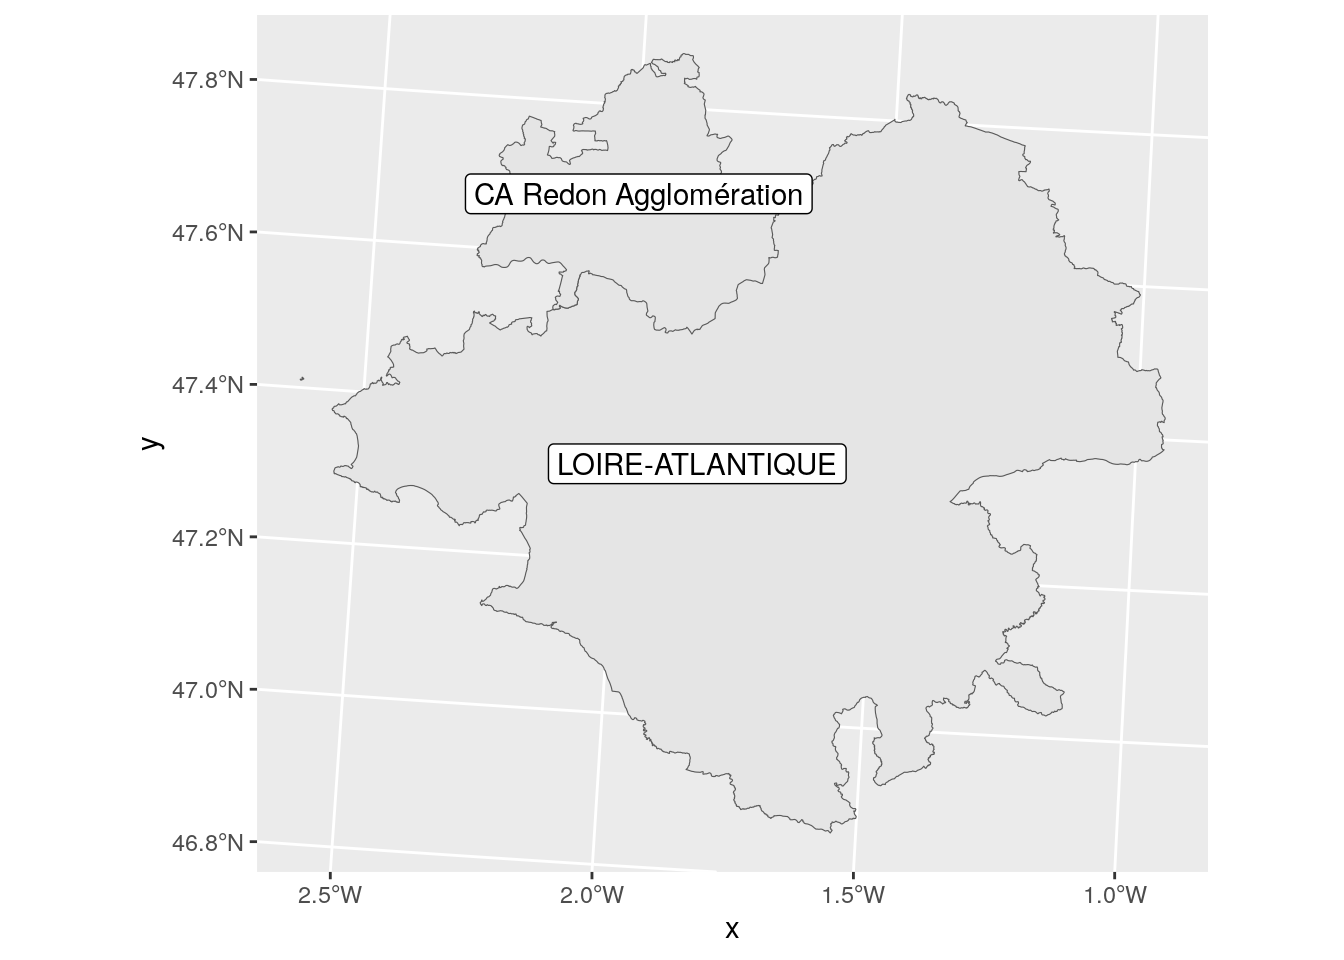
\includegraphics{support_m7_files/figure-latex/unnamed-chunk-78-1.pdf}

Derrière cette opération, \texttt{summarise()} utilise \texttt{st\_union()} du package \texttt{sf} pour dissourdre les polygones des départements en un seul polygone régional.

\begin{Shaded}
\begin{Highlighting}[]
\NormalTok{regions\_52 }\OtherTok{\textless{}{-}}\NormalTok{ departements\_geo }\SpecialCharTok{\%\textgreater{}\%}
  \FunctionTok{filter}\NormalTok{(INSEE\_REG }\SpecialCharTok{==} \StringTok{"52"}\NormalTok{)}

\NormalTok{regions\_52 }\OtherTok{\textless{}{-}} \FunctionTok{st\_union}\NormalTok{(regions\_52)}
\end{Highlighting}
\end{Shaded}

\hypertarget{les-reprojections}{%
\chapter{Les reprojections}\label{les-reprojections}}

Dans ce chapitre, nous allons utiliser les librairies suivantes.

\begin{Shaded}
\begin{Highlighting}[]
\FunctionTok{library}\NormalTok{(sf)}
\FunctionTok{library}\NormalTok{(tidyverse)}
\FunctionTok{library}\NormalTok{(patchwork)}
\FunctionTok{library}\NormalTok{(lwgeom)}
\FunctionTok{library}\NormalTok{(tmap)}
\end{Highlighting}
\end{Shaded}

Pour rappel, il existe deux types de CRS, les CRS géographiques (longitude/lattitude avec pour unité de compte des degrés) et les CRS projetés (avec un datum et une unité en mètre par exemple).

La plupart des fonctions de \texttt{sf} présupposent s'appliquer sur un CRS projeté, car les fonctions de GEOS sur lesquelles elles se basent le font aussi.

\hypertarget{un-premier-exemple-de-reprojection}{%
\section{Un premier exemple de reprojection}\label{un-premier-exemple-de-reprojection}}

Prenons les coordonnées de Nantes en WGS 84:

\begin{Shaded}
\begin{Highlighting}[]
\NormalTok{nantes }\OtherTok{\textless{}{-}} \FunctionTok{data.frame}\NormalTok{(}\AttributeTok{lon =} \SpecialCharTok{{-}}\FloatTok{1.553621}\NormalTok{, }\AttributeTok{lat =} \FloatTok{47.218371}\NormalTok{) }\SpecialCharTok{\%\textgreater{}\%}
  \FunctionTok{st\_as\_sf}\NormalTok{(}\AttributeTok{coords =} \FunctionTok{c}\NormalTok{(}\StringTok{"lon"}\NormalTok{, }\StringTok{"lat"}\NormalTok{)) }\SpecialCharTok{\%\textgreater{}\%}
  \FunctionTok{st\_set\_crs}\NormalTok{(}\DecValTok{4326}\NormalTok{)}
\end{Highlighting}
\end{Shaded}

On peut visualiser nos données

\begin{Shaded}
\begin{Highlighting}[]
\FunctionTok{mapview}\NormalTok{(nantes)}
\end{Highlighting}
\end{Shaded}

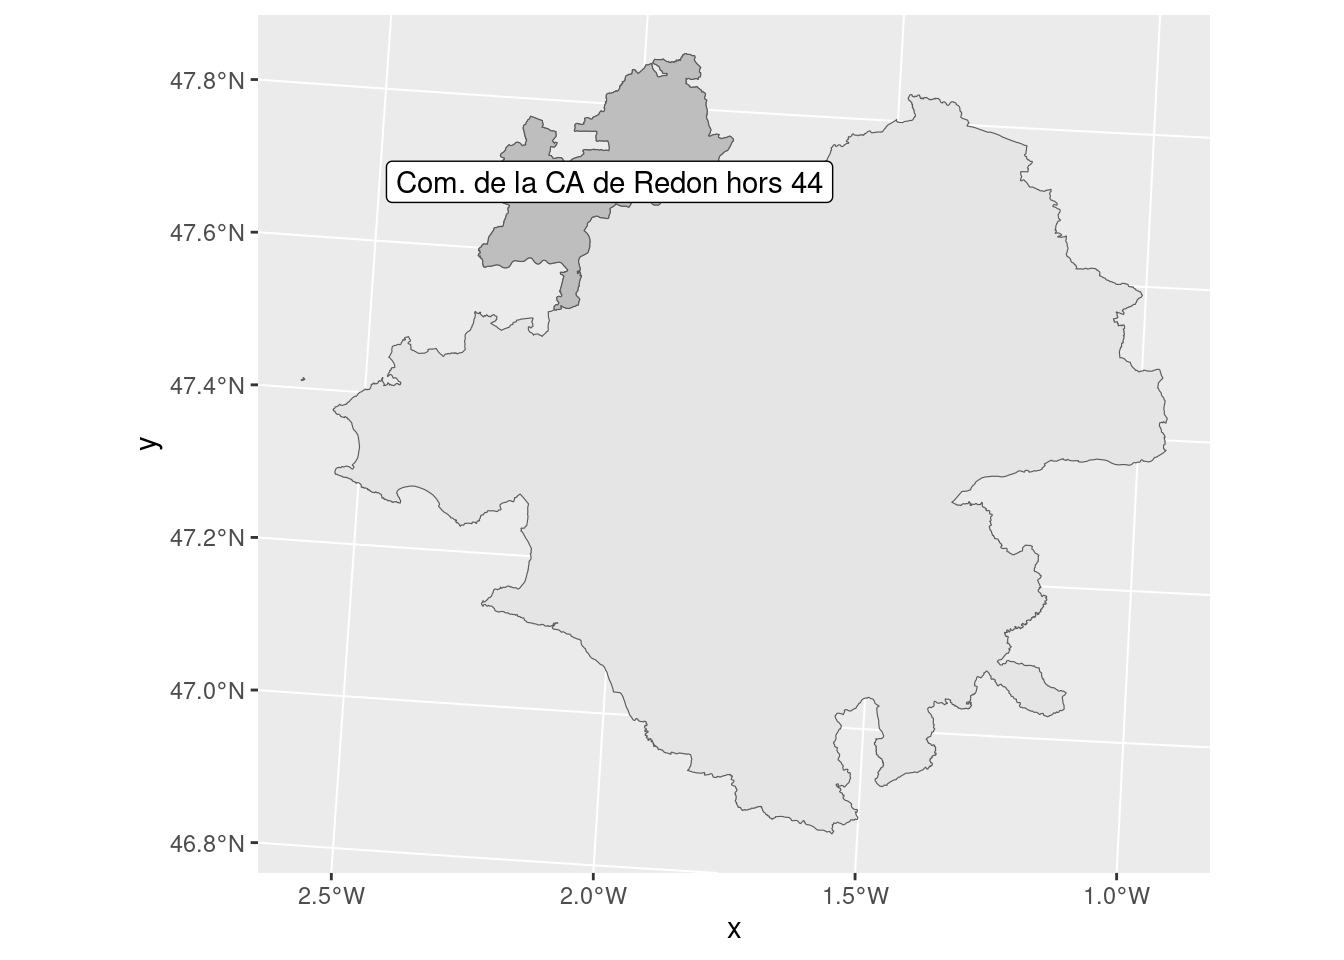
\includegraphics{support_m7_files/figure-latex/unnamed-chunk-82-1.pdf}

\texttt{st\_is\_longlat()} est une fonction de \texttt{sf} qui permet de faire un test sur la famille de CRS à laquelle on a à faire.

\begin{Shaded}
\begin{Highlighting}[]
\FunctionTok{st\_is\_longlat}\NormalTok{(nantes)}
\end{Highlighting}
\end{Shaded}

\begin{verbatim}
[1] TRUE
\end{verbatim}

Essayons de créer un buffer de 1km autour de Nantes

\begin{Shaded}
\begin{Highlighting}[]
\NormalTok{nantes\_buffer }\OtherTok{\textless{}{-}} \FunctionTok{st\_buffer}\NormalTok{(nantes, }\AttributeTok{dist =} \DecValTok{1}\NormalTok{)}
\end{Highlighting}
\end{Shaded}

\begin{Shaded}
\begin{Highlighting}[]
\FunctionTok{mapview}\NormalTok{(}\FunctionTok{list}\NormalTok{(nantes, nantes\_buffer))}
\end{Highlighting}
\end{Shaded}

\includegraphics{support_m7_files/figure-latex/unnamed-chunk-85-1.pdf}

Le message est clair et indique qu'un buffer ne marchera pas correctement sur des données en projection longitude / lattitude.

Tentons une reprojection. La fonction permettant une reprojection est \texttt{st\_transform()}.
On va ici passer en lambert 93 nos données.

\begin{Shaded}
\begin{Highlighting}[]
\NormalTok{nantes\_proj }\OtherTok{\textless{}{-}} \FunctionTok{st\_transform}\NormalTok{(nantes, }\DecValTok{2154}\NormalTok{)}
\end{Highlighting}
\end{Shaded}

Le CRS lambert 93 est bien un CRS projeté :

\begin{Shaded}
\begin{Highlighting}[]
\FunctionTok{st\_is\_longlat}\NormalTok{(nantes\_proj)}
\end{Highlighting}
\end{Shaded}

\begin{verbatim}
[1] FALSE
\end{verbatim}

\begin{Shaded}
\begin{Highlighting}[]
\NormalTok{nantes\_proj\_buffer }\OtherTok{\textless{}{-}} \FunctionTok{st\_buffer}\NormalTok{(nantes\_proj, }\AttributeTok{dist =} \DecValTok{1}\NormalTok{)}
\end{Highlighting}
\end{Shaded}

\begin{Shaded}
\begin{Highlighting}[]
\FunctionTok{mapview}\NormalTok{(}\FunctionTok{list}\NormalTok{(nantes\_proj, nantes\_proj\_buffer))}
\end{Highlighting}
\end{Shaded}

\includegraphics{support_m7_files/figure-latex/unnamed-chunk-89-1.pdf}

\hypertarget{quand-reprojeter}{%
\section{Quand reprojeter ?}\label{quand-reprojeter}}

Quelques cas usuels qui peuvent vous amener à reprojeter vos données :

\begin{itemize}
\item
  la manipulation de données fournies dans des CRS différents
\item
  l'usage du package leaflet impose des données spécifiées en WGS 84
\item
  le besoin de visualiser vos données suivant la conversion de certaines propriétés des objets à la surface de la terre.
\item
  l'usage de fonctions demandant à utiliser des CRS projetés (comme \texttt{st\_buffer()} ci-dessus)
\end{itemize}

Un exemple d'usage : la distance de Rennes à Nantes

Prenons les coordonnées WGS 84 de Rennes

\begin{Shaded}
\begin{Highlighting}[]
\NormalTok{rennes }\OtherTok{\textless{}{-}} \FunctionTok{data.frame}\NormalTok{(}\AttributeTok{lon =} \SpecialCharTok{{-}}\FloatTok{1.6777926}\NormalTok{, }\AttributeTok{lat =} \FloatTok{48.117266}\NormalTok{) }\SpecialCharTok{\%\textgreater{}\%}
  \FunctionTok{st\_as\_sf}\NormalTok{(}\AttributeTok{coords =} \FunctionTok{c}\NormalTok{(}\StringTok{"lon"}\NormalTok{, }\StringTok{"lat"}\NormalTok{)) }\SpecialCharTok{\%\textgreater{}\%}
  \FunctionTok{st\_set\_crs}\NormalTok{(}\DecValTok{4326}\NormalTok{)}
\end{Highlighting}
\end{Shaded}

\begin{Shaded}
\begin{Highlighting}[]
\FunctionTok{mapview}\NormalTok{(rennes)}
\end{Highlighting}
\end{Shaded}

\includegraphics{support_m7_files/figure-latex/unnamed-chunk-91-1.pdf}

Tentons de calculer la distance de Rennes à Nantes.
Avec la données en Lambert 93, la fonction \texttt{st\_distance()} renvoie un message d'erreur.

\begin{Shaded}
\begin{Highlighting}[]
\FunctionTok{st\_distance}\NormalTok{(rennes, nantes\_proj)}
\end{Highlighting}
\end{Shaded}

\begin{verbatim}
Error in st_distance(rennes, nantes_proj): st_crs(x) == st_crs(y) n'est pas TRUE
\end{verbatim}

Avec la données en WGS 84, la fonction \texttt{st\_distance()} renvoie bien le résultat.

\begin{Shaded}
\begin{Highlighting}[]
\FunctionTok{st\_distance}\NormalTok{(rennes, nantes)}
\end{Highlighting}
\end{Shaded}

\begin{verbatim}
Units: [m]
         [,1]
[1,] 100384.2
\end{verbatim}

\hypertarget{quel-crs-utiliser}{%
\section{Quel CRS utiliser ?}\label{quel-crs-utiliser}}

A cette question, il y a rarement une bonne réponse.

En ce qui concerne les CRS géométriques, le plus simple est d'utiliser le WGS 84, qui est de loin le plus populaire, avec lequel beaucoup de données sont fournies.

En ce qui concerne les CRS projetés, utiliser par défaut le lambert 93, le CRS officiel français, pour les données nationales fait sens.

Ensuite votre choix va dépendre des propriétés que vous souhaitez conserver.

\hypertarget{comment-projeter}{%
\section{Comment projeter ?}\label{comment-projeter}}

\hypertarget{projeter-des-vecteurs}{%
\subsection{Projeter des vecteurs}\label{projeter-des-vecteurs}}

Reprojeter des données vecteur se fait à l'aide de la fonction \texttt{st\_transform()} que nous avons vu en utilisant le code epsg que nous voulons.

\hypertarget{modifier-la-projection-dune-carte.}{%
\subsection{Modifier la projection d'une carte.}\label{modifier-la-projection-dune-carte.}}

Parfois on souhaite pouvoir aller plus loin dans les reprojections, en adaptant le centre de la projection, pour cela on peut utiliser un \texttt{proj4string} ad hoc.

Pour cela, on va modifier l'argument \texttt{+proj} de notre crs avec \texttt{st\_transform}.

Tentons par exemple de reprojeter notre carte du globe en utilisant la projection azimutale équivalente de Lambert, centrée sur Pékin.

\begin{Shaded}
\begin{Highlighting}[]
\FunctionTok{data}\NormalTok{(}\StringTok{"World"}\NormalTok{)}
\NormalTok{World\_pekin }\OtherTok{\textless{}{-}} \FunctionTok{st\_transform}\NormalTok{(World, }\AttributeTok{crs =} \StringTok{"+proj=laea +x\_0=0 +y\_0=0 +lon\_0=116 +lat\_0=40"}\NormalTok{)}
\end{Highlighting}
\end{Shaded}

Le paramètre \texttt{+proj=laea} permet de redéfinir la projection, les paramètres \texttt{+lon\_0} et \texttt{lat\_0} permettent de définir le centre de la projection. \texttt{x\_0} et \texttt{y\_0} définissent le centre du plan pour les coordonnées.

Qu'est ce qui a changé entre nos deux cartes ?

\begin{Shaded}
\begin{Highlighting}[]
\FunctionTok{st\_crs}\NormalTok{(World)}
\end{Highlighting}
\end{Shaded}

\begin{verbatim}
Coordinate Reference System:
  User input: EPSG:4326 
  wkt:
GEOGCRS["WGS 84",
    DATUM["World Geodetic System 1984",
        ELLIPSOID["WGS 84",6378137,298.257223563,
            LENGTHUNIT["metre",1]]],
    PRIMEM["Greenwich",0,
        ANGLEUNIT["degree",0.0174532925199433]],
    CS[ellipsoidal,2],
        AXIS["geodetic latitude (Lat)",north,
            ORDER[1],
            ANGLEUNIT["degree",0.0174532925199433]],
        AXIS["geodetic longitude (Lon)",east,
            ORDER[2],
            ANGLEUNIT["degree",0.0174532925199433]],
    USAGE[
        SCOPE["unknown"],
        AREA["World"],
        BBOX[-90,-180,90,180]],
    ID["EPSG",4326]]
\end{verbatim}

\begin{Shaded}
\begin{Highlighting}[]
\FunctionTok{st\_crs}\NormalTok{(World\_pekin)}
\end{Highlighting}
\end{Shaded}

\begin{verbatim}
Coordinate Reference System:
  User input: +proj=laea +x_0=0 +y_0=0 +lon_0=116 +lat_0=40 
  wkt:
PROJCRS["unknown",
    BASEGEOGCRS["unknown",
        DATUM["World Geodetic System 1984",
            ELLIPSOID["WGS 84",6378137,298.257223563,
                LENGTHUNIT["metre",1]],
            ID["EPSG",6326]],
        PRIMEM["Greenwich",0,
            ANGLEUNIT["degree",0.0174532925199433],
            ID["EPSG",8901]]],
    CONVERSION["unknown",
        METHOD["Lambert Azimuthal Equal Area",
            ID["EPSG",9820]],
        PARAMETER["Latitude of natural origin",40,
            ANGLEUNIT["degree",0.0174532925199433],
            ID["EPSG",8801]],
        PARAMETER["Longitude of natural origin",116,
            ANGLEUNIT["degree",0.0174532925199433],
            ID["EPSG",8802]],
        PARAMETER["False easting",0,
            LENGTHUNIT["metre",1],
            ID["EPSG",8806]],
        PARAMETER["False northing",0,
            LENGTHUNIT["metre",1],
            ID["EPSG",8807]]],
    CS[Cartesian,2],
        AXIS["(E)",east,
            ORDER[1],
            LENGTHUNIT["metre",1,
                ID["EPSG",9001]]],
        AXIS["(N)",north,
            ORDER[2],
            LENGTHUNIT["metre",1,
                ID["EPSG",9001]]]]
\end{verbatim}

\includegraphics{support_m7_files/figure-latex/unnamed-chunk-96-1.pdf}

\hypertarget{part-cruxe9er-des-cartes-sous-r}{%
\part{Créer des cartes sous R}\label{part-cruxe9er-des-cartes-sous-r}}

\hypertarget{cruxe9er-des-cartes-avec-ggplot2}{%
\chapter{Créer des cartes avec ggplot2}\label{cruxe9er-des-cartes-avec-ggplot2}}

Dans ce chapitre, nous allons utiliser les librairies suivantes.

\begin{Shaded}
\begin{Highlighting}[]
\FunctionTok{library}\NormalTok{(sf)}
\FunctionTok{library}\NormalTok{(tidyverse)}
\FunctionTok{library}\NormalTok{(ggplot2)}
\FunctionTok{library}\NormalTok{(patchwork)}
\FunctionTok{library}\NormalTok{(lwgeom)}
\CommentTok{\#remotes::install\_github("MaelTheuliere/variousdata")}
\FunctionTok{library}\NormalTok{(variousdata)}
\FunctionTok{library}\NormalTok{(ggspatial)}
\end{Highlighting}
\end{Shaded}

\hypertarget{quelques-rappels-sur-ggplot2}{%
\section{Quelques rappels sur ggplot2}\label{quelques-rappels-sur-ggplot2}}

\hypertarget{pruxe9sentation-du-package-ggplot2}{%
\subsection{Présentation du package ggplot2}\label{pruxe9sentation-du-package-ggplot2}}

\begin{itemize}
\item
  \href{http://ggplot2.tidyverse.org/}{ggplot 2} est un package créé par Hadley Wickham et Winston Chang pour implémenter dans R la vision développée par Leland Wilkinson dans \href{https://www.amazon.com/Grammar-Graphics-Statistics-Computing/dp/0387245448/ref=as_li_ss_tl?ie=UTF8\&qid=1477928463\&sr=8-1\&keywords=the+grammar+of+graphics\&linkCode=sl1\&tag=ggplot2-20\&linkId=f0130e557161b83fbe97ba0e9175c431}{The Grammar of Graphics (Statistics and Computing)} de la conception de graphiques.
\item
  Le but est de fournir une approche unique pour produire quasiment \textbf{toute valorisation graphique} de données que l'on peut trouver dans des revues scientifiques, les journaux, dans l'analyse statistique ou la data visualisation.
\item
  Ce package aujourd'hui s'inscrit dans R dans le \textbf{framework Tidyverse} qui propose une approche cohérente sur l'ensemble de la chaîne de vie de la donnée : importation, préparation des données, analyse et valorisation.
\end{itemize}

\hypertarget{le-tidyverse}{%
\subsection{Le Tidyverse}\label{le-tidyverse}}

\begin{figure}
\hypertarget{id}{%
\centering
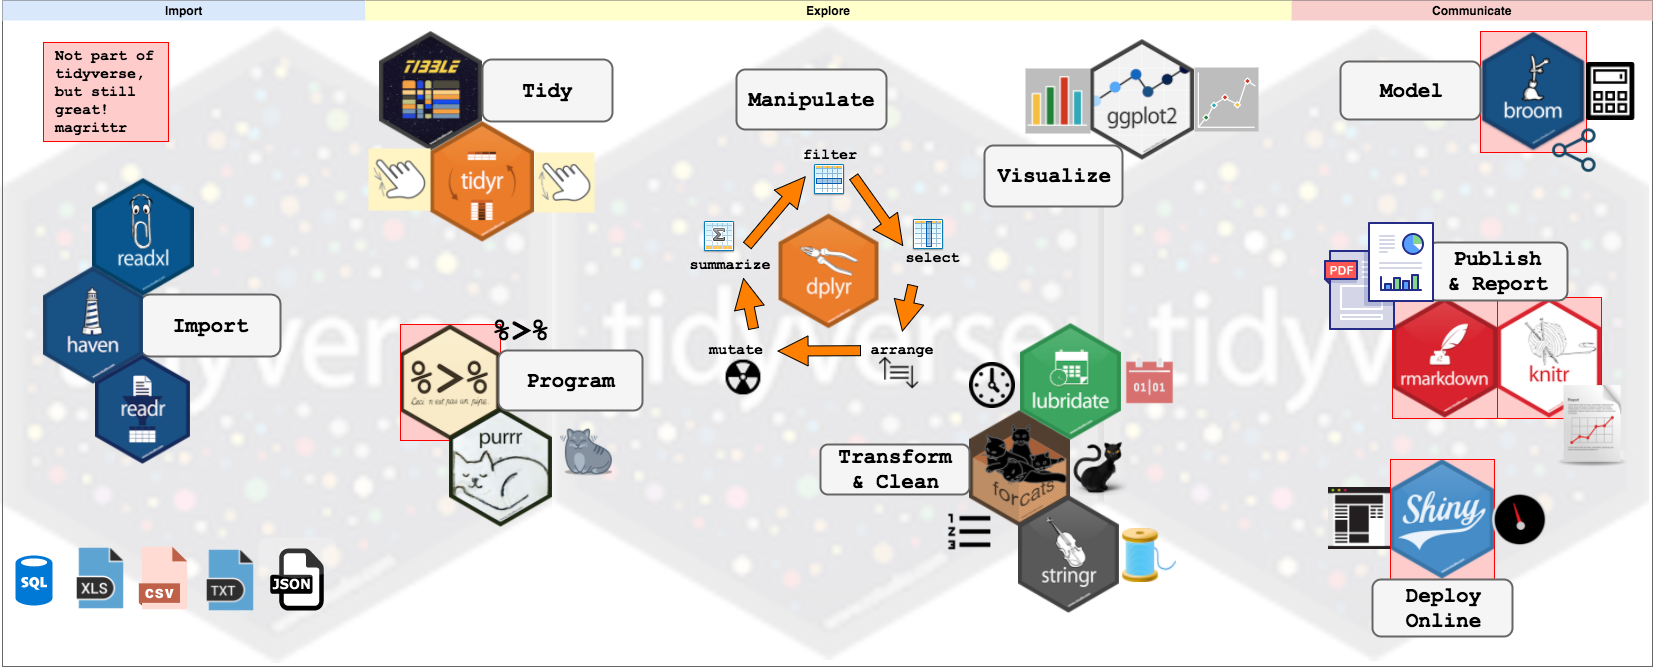
\includegraphics[width=8.33333in,height=\textheight]{pic/tidyverse.png}
\caption{le tidyverse}\label{id}
}
\end{figure}

\hypertarget{ggplot-2-les-concepts-clefs}{%
\subsection{ggplot 2 : les concepts clefs}\label{ggplot-2-les-concepts-clefs}}

Pour construire un graphique avec ggplot il va falloir lui définir plusieurs éléments :

\begin{itemize}
\item
  \textbf{la donnée} : ggplot2 permet de travailler sur des vecteurs, des dataframes, des tibbles, ou des données spatiales ;
\item
  le \textbf{mapping} : on définit dans l'aesthetic (ou aes) le \textbf{mapping}, c'est à dire ce que l'on veut représenter qui \textbf{dépend des variables} (quelle variable sur l'axe x, sur l'axe y, quelle variable pour définir une graduation de couleurs\ldots) ;
\item
  les \textbf{paramètres} : on définit les autres paramètres qui dépendent de constantes (par exemple : je veux que toutes mes lignes soient rouges ou de taille 2 pixels) ;
\item
  le \textbf{layer (``forme géométrique'')} : on définit sous quelle représentation graphique on représente les paramètres précédents. Sous ggplot, ces fonctions sont de la forme geom\_XX ;
\end{itemize}

L'écriture type d'un graphique sera donc:

\begin{Shaded}
\begin{Highlighting}[]
\FunctionTok{ggplot}\NormalTok{(}\AttributeTok{data =} \SpecialCharTok{\textless{}}\NormalTok{DATA}\SpecialCharTok{\textgreater{}}\NormalTok{) }\SpecialCharTok{+} 
  \ErrorTok{\textless{}}\NormalTok{FORME\_GEO}\SpecialCharTok{\textgreater{}}\NormalTok{(}\AttributeTok{mapping =} \FunctionTok{aes}\NormalTok{(}\SpecialCharTok{\textless{}}\NormalTok{MAPPINGS}\SpecialCharTok{\textgreater{}}\NormalTok{),}\AttributeTok{...=}\SpecialCharTok{\textless{}}\NormalTok{PARAMS}\SpecialCharTok{\textgreater{}}\NormalTok{)}
\end{Highlighting}
\end{Shaded}

On va ensuite pouvoir partir de cette base pour l'enrichir avec des fonctions supplémentaires.
Chaque fonction s'enchaine avec des \texttt{+} comme les \texttt{\%\textgreater{}\%}.

\begin{Shaded}
\begin{Highlighting}[]
\FunctionTok{ggplot}\NormalTok{(}\AttributeTok{data =} \SpecialCharTok{\textless{}}\NormalTok{DATA}\SpecialCharTok{\textgreater{}}\NormalTok{) }\SpecialCharTok{+} 
  \ErrorTok{\textless{}}\NormalTok{FORME\_GEO}\SpecialCharTok{\textgreater{}}\NormalTok{(}\AttributeTok{mapping =} \FunctionTok{aes}\NormalTok{(}\SpecialCharTok{\textless{}}\NormalTok{MAPPINGS}\SpecialCharTok{\textgreater{}}\NormalTok{),}\AttributeTok{...=}\SpecialCharTok{\textless{}}\NormalTok{PARAMS}\SpecialCharTok{\textgreater{}}\NormalTok{)}\SpecialCharTok{+}
  \ErrorTok{\textless{}}\NormalTok{FONCTION1}\SpecialCharTok{\textgreater{}+}
\NormalTok{  ...}
\end{Highlighting}
\end{Shaded}

\hypertarget{le-mapping}{%
\subsection{Le mapping}\label{le-mapping}}

\hypertarget{les-paramuxe8tres-du-mapping}{%
\subsubsection{Les paramètres du mapping}\label{les-paramuxe8tres-du-mapping}}

Dans l'exemple qui suit, la représentation géographique utilisée est le nuage de point \texttt{geom\_point()}.
D'autres types de représentations graphiques sont présentées dans la partie suivante.

L'aesthetic sert à identifier les variables que l'on souhaite représenter.
Par exemple, si l'on souhaite représenter le taux de mortalité maternelle (Maternal\_mortality\_ratio) en fonction du produit intérieur brut (Gross\_Domestic\_Product\_GDP) :

\begin{Shaded}
\begin{Highlighting}[]
\NormalTok{sdg\_indicators }\SpecialCharTok{\%\textgreater{}\%} 
  \FunctionTok{filter}\NormalTok{(timeperiod }\SpecialCharTok{==}\DecValTok{2015}\NormalTok{) }\SpecialCharTok{\%\textgreater{}\%} 
  \FunctionTok{ggplot}\NormalTok{() }\SpecialCharTok{+}
    \FunctionTok{geom\_point}\NormalTok{(}\FunctionTok{aes}\NormalTok{(}\AttributeTok{x =}\NormalTok{ gdp\_per\_cap, }\AttributeTok{y =}\NormalTok{ sh\_sta\_mmr))}
\end{Highlighting}
\end{Shaded}

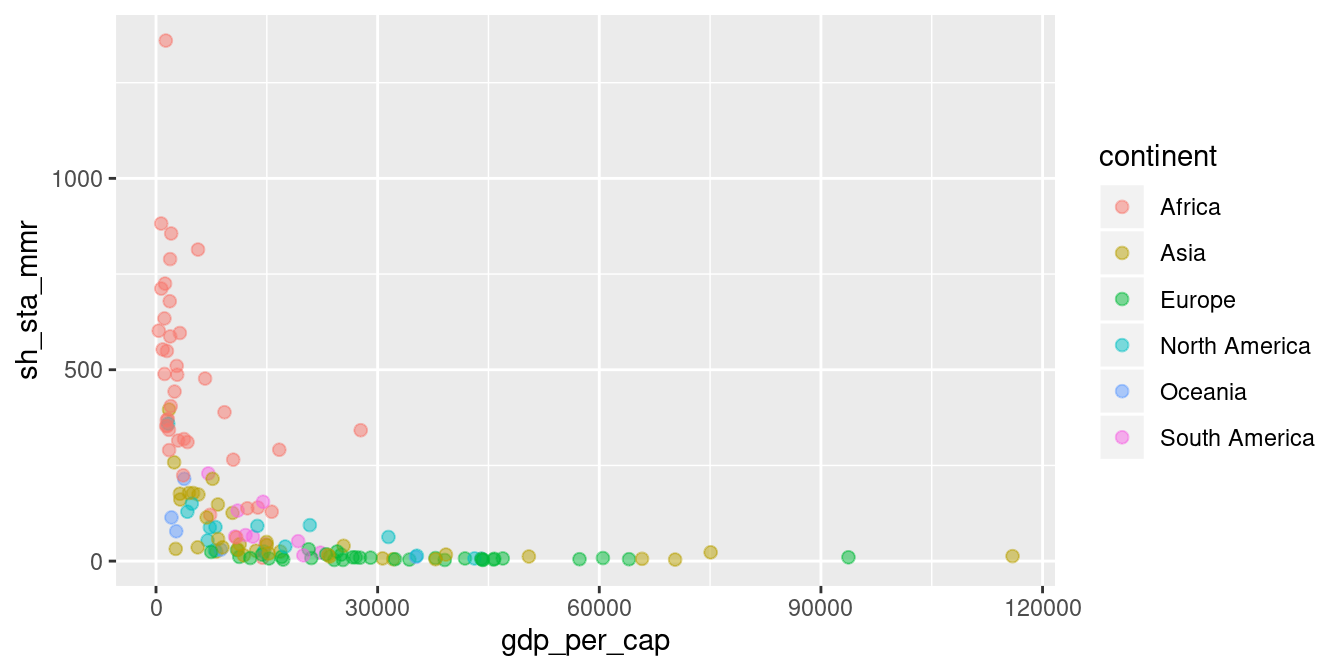
\includegraphics{support_m7_files/figure-latex/unnamed-chunk-101-1.pdf}

De plus, la fonction \texttt{aes()} admet d'autres arguments qui permettent de modifier l'apparence du graphique selon une 3ème variable du jeu de données.

\begin{itemize}
\tightlist
\item
  \texttt{colour} : la couleur,
\item
  \texttt{shape} : la forme,
\item
  \texttt{size} : la taille,
\item
  \texttt{alpha} : la transparence,
\item
  \texttt{fill} : le remplissage ;
\end{itemize}

\begin{Shaded}
\begin{Highlighting}[]
\NormalTok{sdg\_indicators }\SpecialCharTok{\%\textgreater{}\%} 
  \FunctionTok{filter}\NormalTok{(timeperiod }\SpecialCharTok{==}\DecValTok{2015}\NormalTok{) }\SpecialCharTok{\%\textgreater{}\%} 
  \FunctionTok{ggplot}\NormalTok{() }\SpecialCharTok{+}
  \FunctionTok{geom\_point}\NormalTok{(}\FunctionTok{aes}\NormalTok{(}\AttributeTok{x =}\NormalTok{ gdp\_per\_cap, }
                 \AttributeTok{y =}\NormalTok{ sh\_sta\_mmr,}
                 \AttributeTok{color =}\NormalTok{ continent))}
\end{Highlighting}
\end{Shaded}

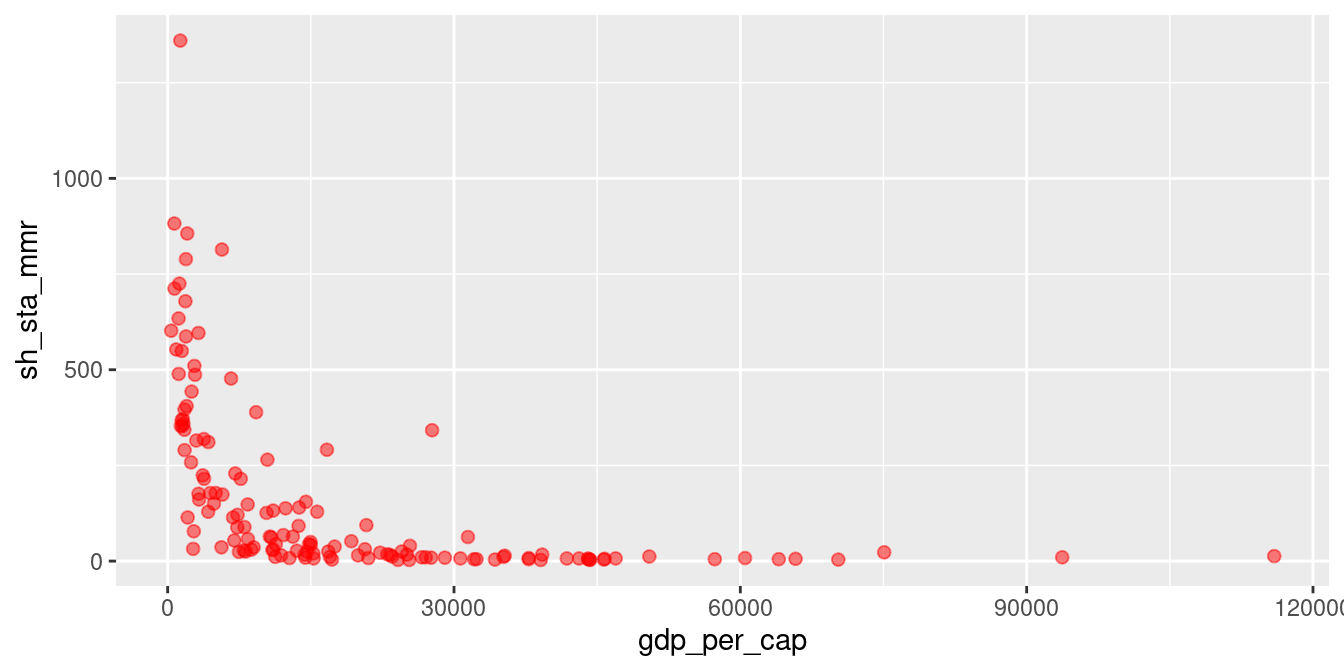
\includegraphics{support_m7_files/figure-latex/unnamed-chunk-102-1.pdf}

\hypertarget{les-autres-paramuxe8tres}{%
\subsubsection{Les ``autres'' paramètres}\label{les-autres-paramuxe8tres}}

Il est possible de spécifier des paramètres qui seront valables pour l'ensemble du graphique.
On retrouve entre autre les mêmes paramètres que proposés dans l'aes mais il faut alors les passer \textbf{en dehors de l'aesthetic}.

Par exemple si l'on souhaite modifier la transparance et la taille de l'ensemble des points du graphique précédent:

\begin{Shaded}
\begin{Highlighting}[]
\NormalTok{sdg\_indicators }\SpecialCharTok{\%\textgreater{}\%} 
  \FunctionTok{filter}\NormalTok{(timeperiod }\SpecialCharTok{==}\DecValTok{2015}\NormalTok{) }\SpecialCharTok{\%\textgreater{}\%} 
  \FunctionTok{ggplot}\NormalTok{() }\SpecialCharTok{+}
  \FunctionTok{geom\_point}\NormalTok{(}\FunctionTok{aes}\NormalTok{(}\AttributeTok{x =}\NormalTok{ gdp\_per\_cap, }
                 \AttributeTok{y =}\NormalTok{ sh\_sta\_mmr,}
                 \AttributeTok{color =}\NormalTok{ continent),}
    \AttributeTok{alpha =} \FloatTok{0.5}\NormalTok{, }
    \AttributeTok{size =} \FloatTok{1.9}
\NormalTok{  )}
\end{Highlighting}
\end{Shaded}

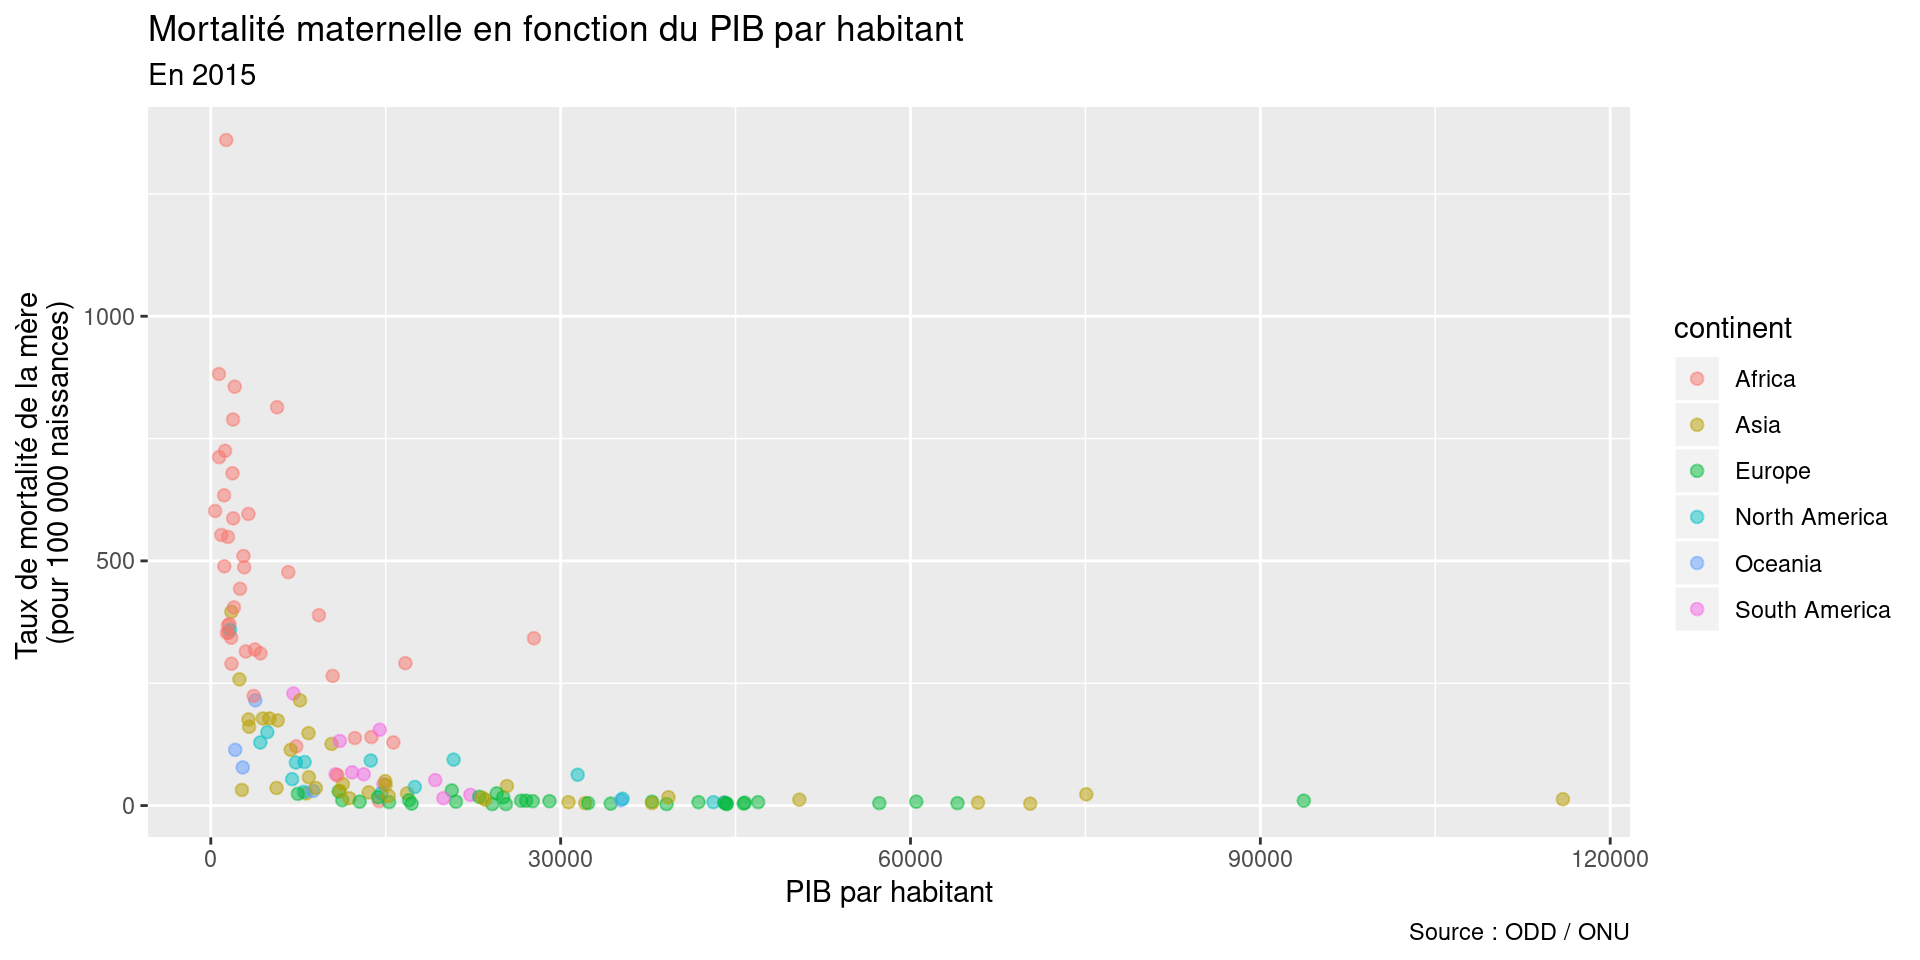
\includegraphics{support_m7_files/figure-latex/unnamed-chunk-103-1.pdf}

De même si l'on souhaite modifier la couleur générale:

\begin{Shaded}
\begin{Highlighting}[]
\NormalTok{sdg\_indicators }\SpecialCharTok{\%\textgreater{}\%} 
  \FunctionTok{filter}\NormalTok{(timeperiod }\SpecialCharTok{==}\DecValTok{2015}\NormalTok{) }\SpecialCharTok{\%\textgreater{}\%} 
  \FunctionTok{ggplot}\NormalTok{() }\SpecialCharTok{+}
  \FunctionTok{geom\_point}\NormalTok{(}\FunctionTok{aes}\NormalTok{(}\AttributeTok{x =}\NormalTok{ gdp\_per\_cap, }
                 \AttributeTok{y =}\NormalTok{ sh\_sta\_mmr),}
    \AttributeTok{color =} \StringTok{"red"}\NormalTok{,}
    \AttributeTok{alpha =} \FloatTok{0.5}\NormalTok{, }
    \AttributeTok{size =} \FloatTok{1.9}
\NormalTok{  )}
\end{Highlighting}
\end{Shaded}

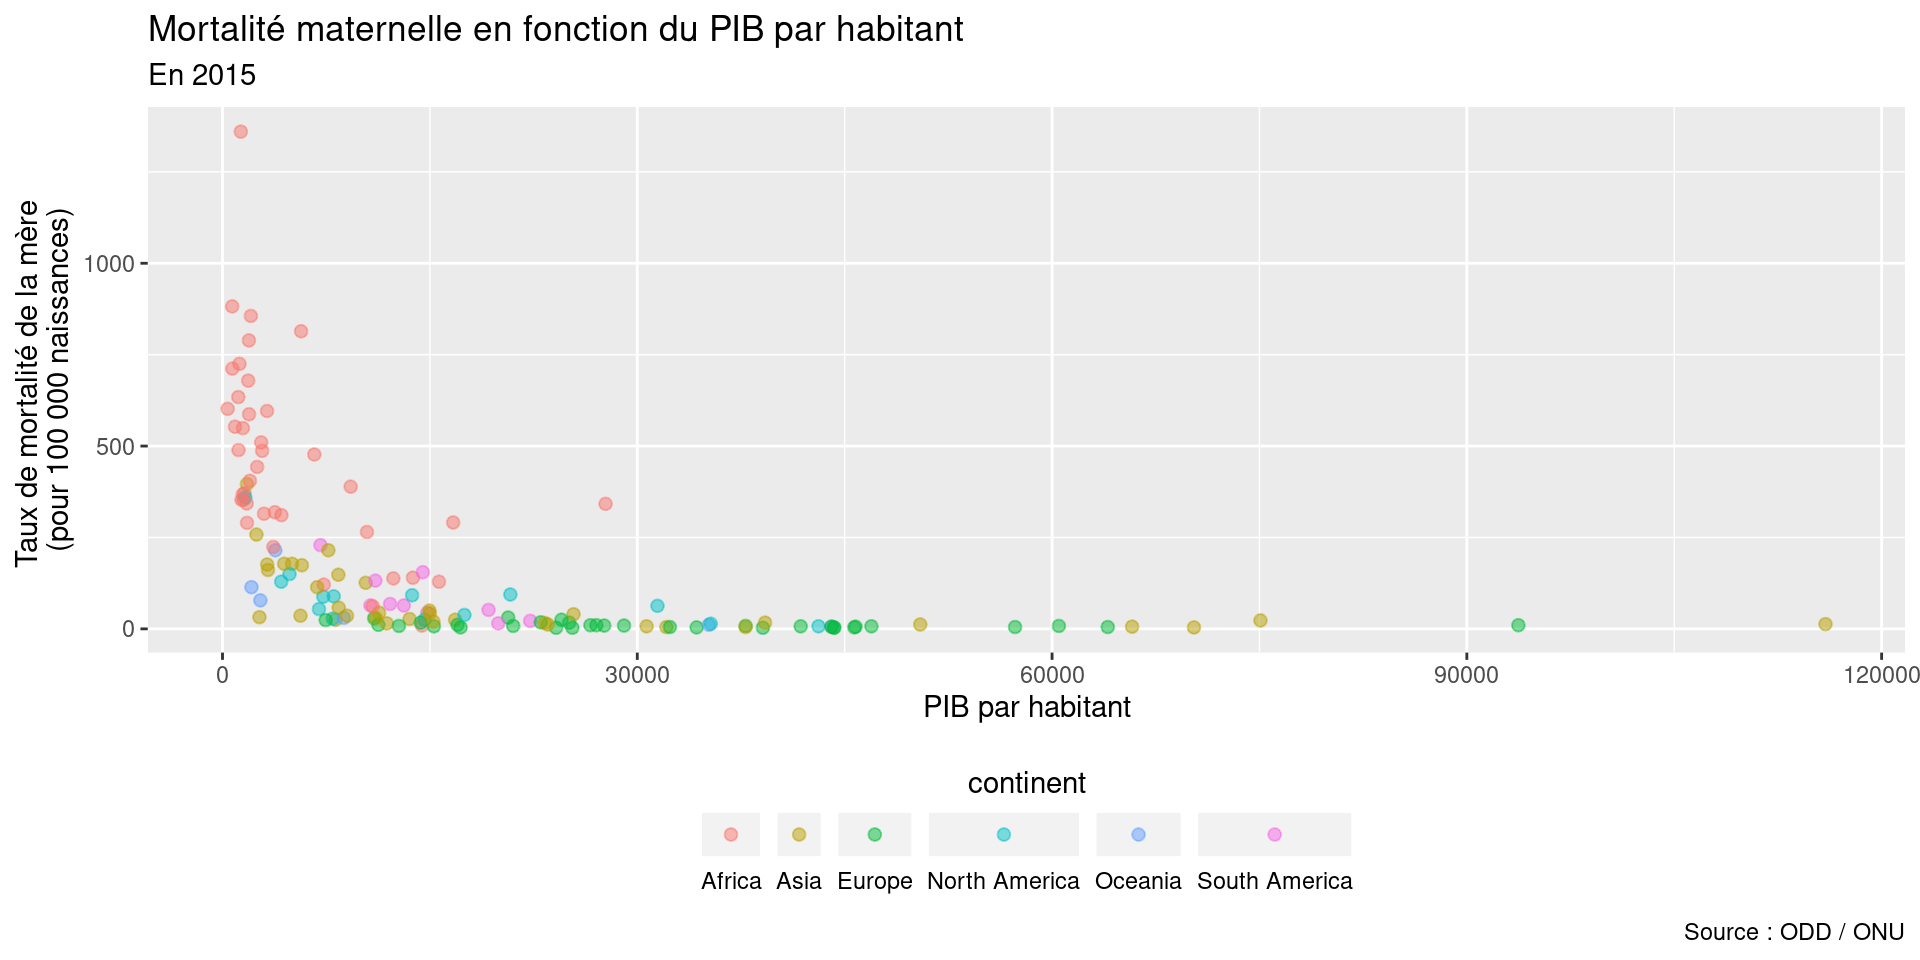
\includegraphics{support_m7_files/figure-latex/unnamed-chunk-104-1.pdf}

Pour choisir et modifier facilement les couleurs d'un graphique, il existe un addin développé par Dean Attali: \texttt{Colour\ Picker}.

Il est installable comme n'importe quel package.

Pour plus d'informations: \url{https://github.com/daattali/colourpicker}

\hypertarget{lhabillage-simple}{%
\subsection{L'habillage simple}\label{lhabillage-simple}}

\hypertarget{titre-et-libelluxe9-des-axes}{%
\subsubsection{Titre et libellé des axes}\label{titre-et-libelluxe9-des-axes}}

Chaque nouvel élément graphique est à rajouter sous forme de layer, ici nous utilisons la fonction \texttt{labs()} qui permet de labelliser tout les éléments possibles de l'aesthétic, ainsi que le titre (\texttt{title}), le sous titre (\texttt{subtitle}) et le bas de page (\texttt{caption})

\begin{Shaded}
\begin{Highlighting}[]
\NormalTok{sdg\_indicators }\SpecialCharTok{\%\textgreater{}\%} 
  \FunctionTok{filter}\NormalTok{(timeperiod }\SpecialCharTok{==}\DecValTok{2015}\NormalTok{) }\SpecialCharTok{\%\textgreater{}\%} 
  \FunctionTok{ggplot}\NormalTok{() }\SpecialCharTok{+}
  \FunctionTok{geom\_point}\NormalTok{(}\FunctionTok{aes}\NormalTok{(}\AttributeTok{x =}\NormalTok{ gdp\_per\_cap, }
                 \AttributeTok{y =}\NormalTok{ sh\_sta\_mmr,}
                 \AttributeTok{color =}\NormalTok{ continent),}
    \AttributeTok{alpha =} \FloatTok{0.5}\NormalTok{, }
    \AttributeTok{size =} \FloatTok{1.9}
\NormalTok{  ) }\SpecialCharTok{+}
  \FunctionTok{labs}\NormalTok{(}
    \AttributeTok{title =} \StringTok{"Mortalité maternelle en fonction du PIB par habitant"}\NormalTok{,}
    \AttributeTok{subtitle =} \StringTok{"En 2015"}\NormalTok{,}
    \AttributeTok{x =} \StringTok{"PIB par habitant"}\NormalTok{,}
    \AttributeTok{y =} \StringTok{"Taux de mortalité de la mère }\SpecialCharTok{\textbackslash{}n}\StringTok{(pour 100 000 naissances)"}\NormalTok{,}
    \AttributeTok{caption =} \StringTok{"Source : ODD / ONU"}
\NormalTok{  )}
\end{Highlighting}
\end{Shaded}

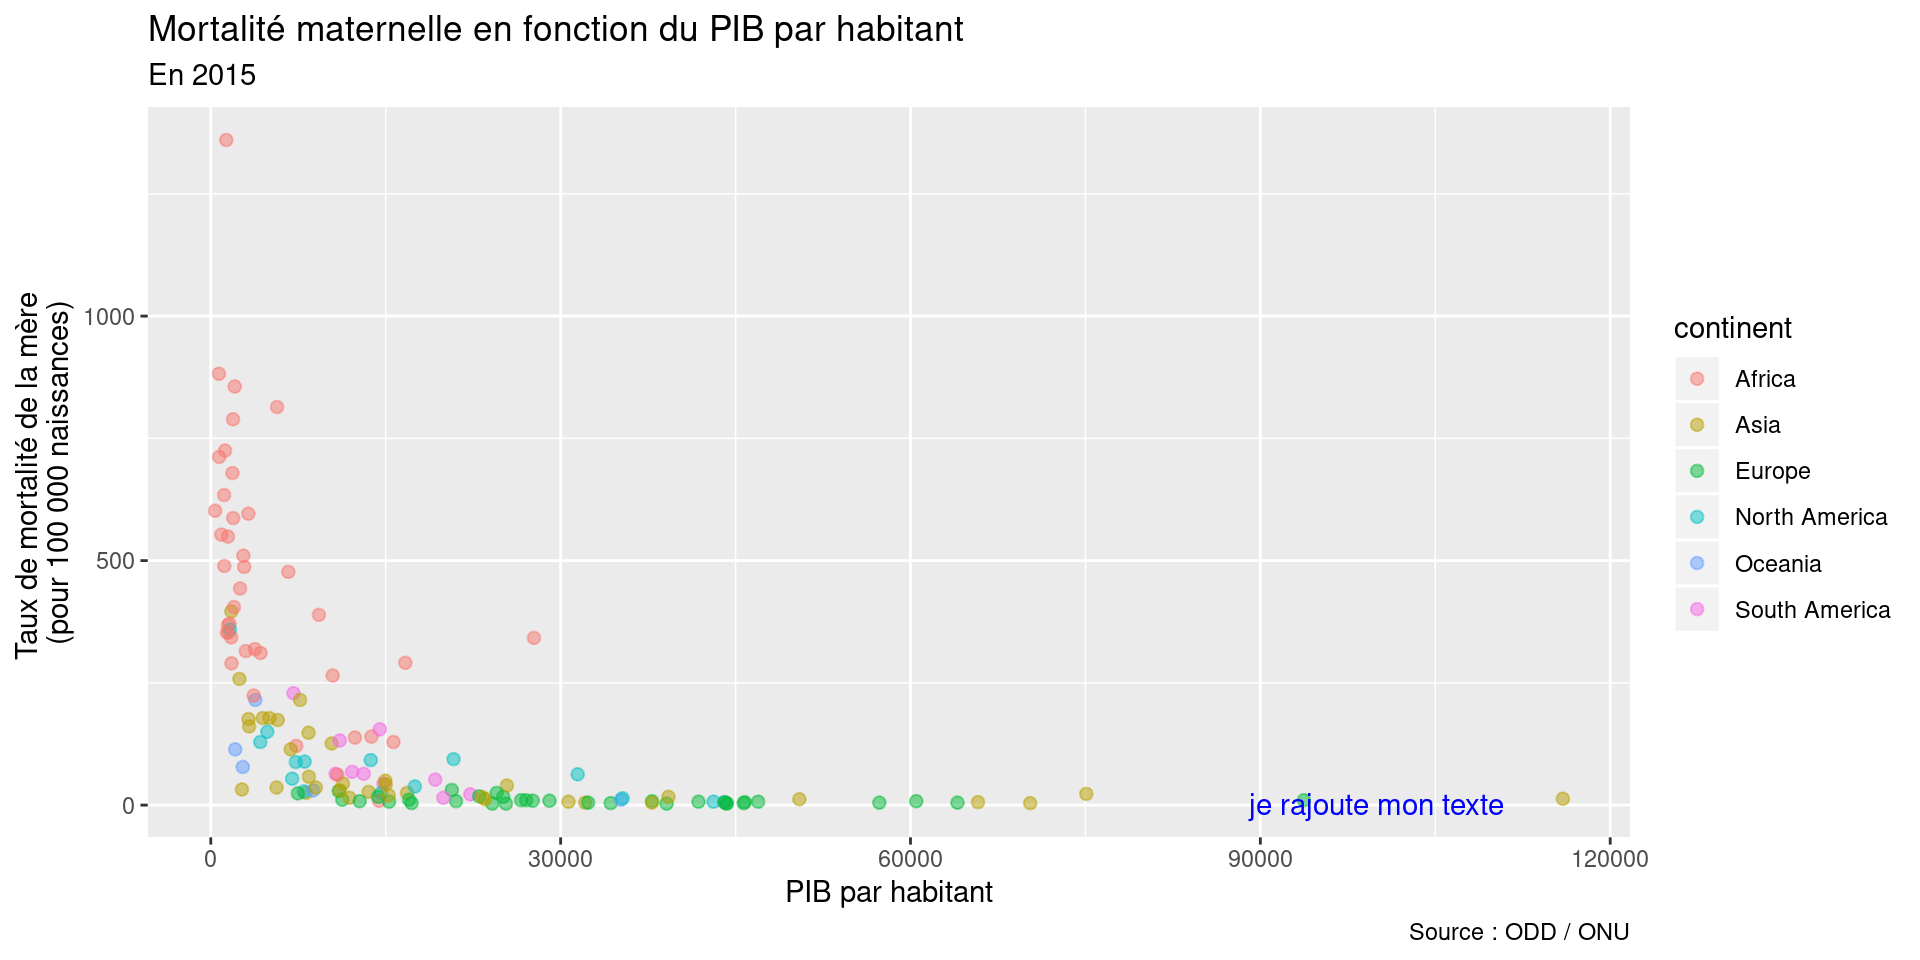
\includegraphics{support_m7_files/figure-latex/unnamed-chunk-105-1.pdf}

A noter qu'il existe plusieurs autres façons de spécifier ces élèments par des fonctions spécifiques: ggtitle, xlab, ylab,\ldots{}

\hypertarget{luxe9gende}{%
\subsubsection{Légende}\label{luxe9gende}}

Les fonctions \texttt{guide()} et \texttt{guides} permettent de modifier finement la légende.
Les guides peuvent être spécifiées dans chaque \texttt{scale\_} ou dans une instruction \texttt{guides}.

\begin{Shaded}
\begin{Highlighting}[]
\NormalTok{sdg\_indicators }\SpecialCharTok{\%\textgreater{}\%} 
  \FunctionTok{filter}\NormalTok{(timeperiod }\SpecialCharTok{==}\DecValTok{2015}\NormalTok{) }\SpecialCharTok{\%\textgreater{}\%} 
  \FunctionTok{ggplot}\NormalTok{() }\SpecialCharTok{+}
  \FunctionTok{geom\_point}\NormalTok{(}\FunctionTok{aes}\NormalTok{(}\AttributeTok{x =}\NormalTok{ gdp\_per\_cap, }
                 \AttributeTok{y =}\NormalTok{ sh\_sta\_mmr,}
                 \AttributeTok{color =}\NormalTok{ continent),}
    \AttributeTok{alpha =} \FloatTok{0.5}\NormalTok{, }
    \AttributeTok{size =} \FloatTok{1.9}
\NormalTok{  ) }\SpecialCharTok{+}
  \FunctionTok{labs}\NormalTok{(}
    \AttributeTok{title =} \StringTok{"Mortalité maternelle en fonction du PIB par habitant"}\NormalTok{,}
    \AttributeTok{subtitle =} \StringTok{"En 2015"}\NormalTok{,}
    \AttributeTok{x =} \StringTok{"PIB par habitant"}\NormalTok{,}
    \AttributeTok{y =} \StringTok{"Taux de mortalité de la mère }\SpecialCharTok{\textbackslash{}n}\StringTok{(pour 100 000 naissances)"}\NormalTok{,}
    \AttributeTok{caption =} \StringTok{"Source : ODD / ONU"}
\NormalTok{  ) }\SpecialCharTok{+}
  \FunctionTok{guides}\NormalTok{(}\AttributeTok{color =} \FunctionTok{guide\_legend}\NormalTok{(}
    \AttributeTok{direction =} \StringTok{"horizontal"}\NormalTok{,}
    \AttributeTok{order =} \DecValTok{1}\NormalTok{,}
    \AttributeTok{title.position =} \StringTok{"top"}\NormalTok{,}
    \AttributeTok{title.hjust =} \FloatTok{0.5}\NormalTok{,}
    \AttributeTok{nrow =} \DecValTok{1}\NormalTok{,}
    \AttributeTok{label.position =} \StringTok{"bottom"}
\NormalTok{  )) }\SpecialCharTok{+}
  \FunctionTok{theme}\NormalTok{(}\AttributeTok{legend.position =} \StringTok{"bottom"}\NormalTok{)}
\end{Highlighting}
\end{Shaded}

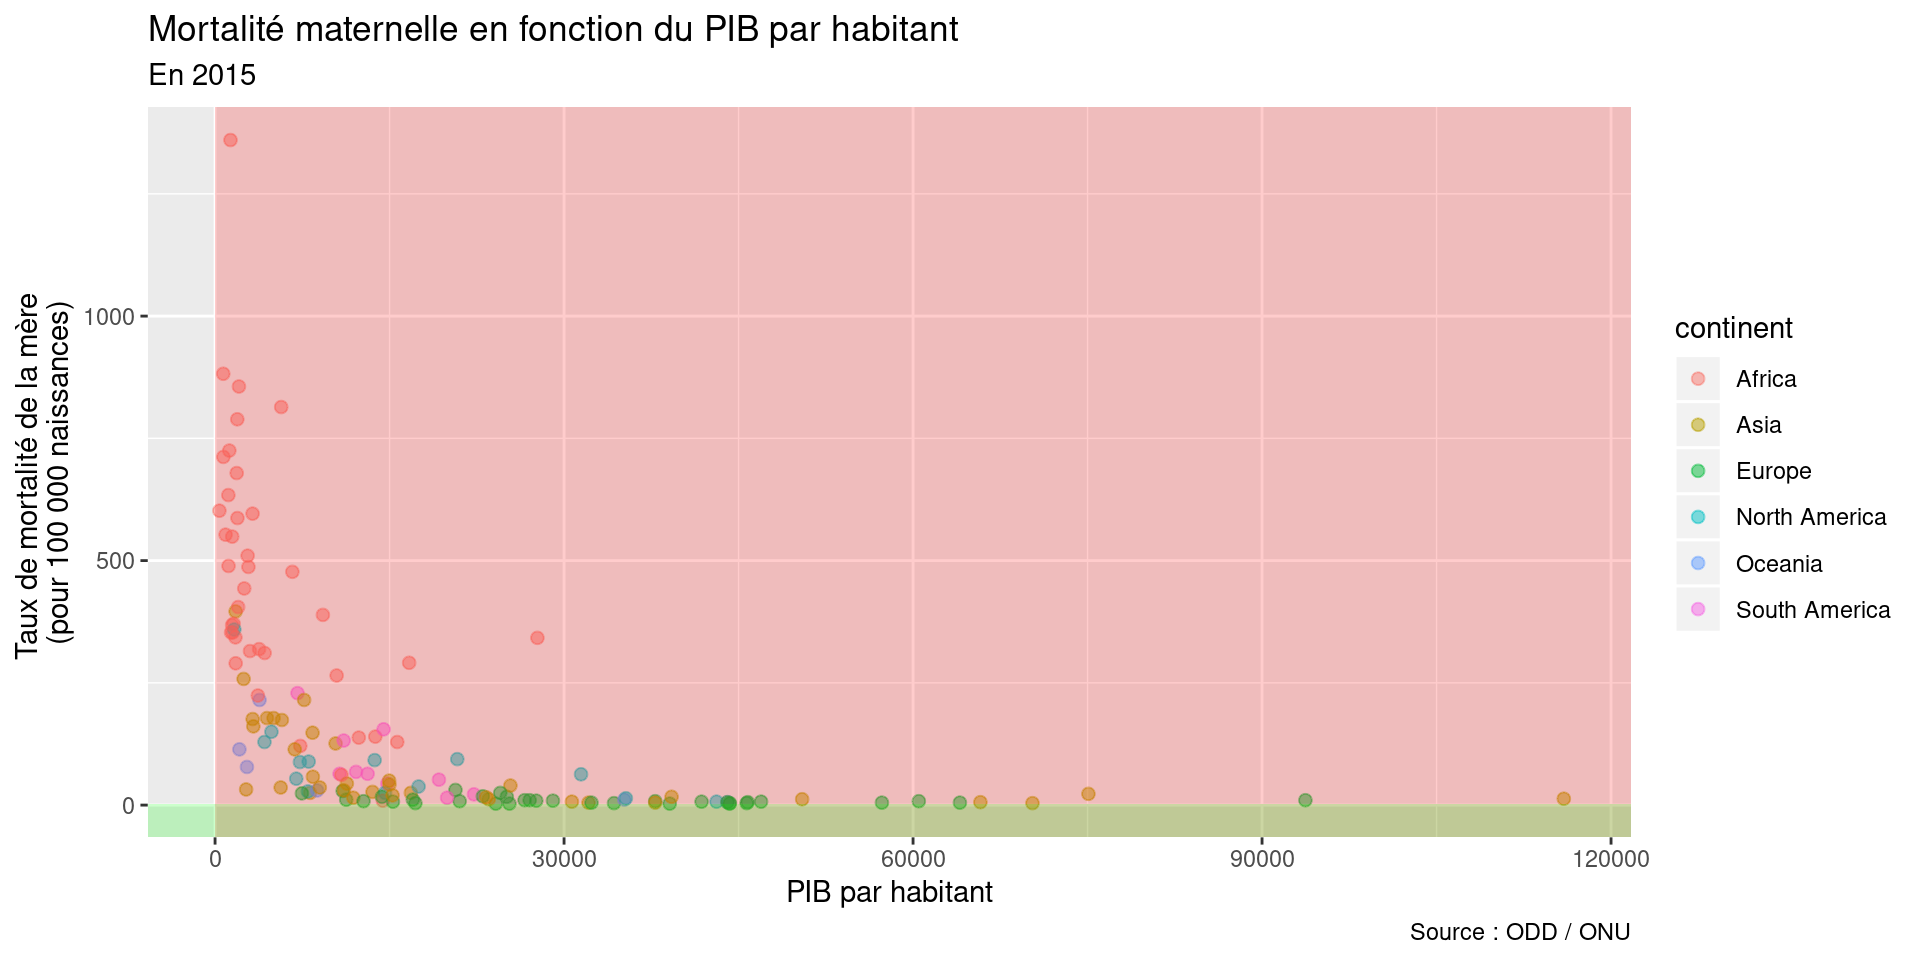
\includegraphics{support_m7_files/figure-latex/unnamed-chunk-106-1.pdf}

\hypertarget{annotation}{%
\subsubsection{Annotation}\label{annotation}}

Il est aussi possible de rajouter des annotations de type texte, par exemple, ``à la volée.''

\begin{Shaded}
\begin{Highlighting}[]
\NormalTok{sdg\_indicators }\SpecialCharTok{\%\textgreater{}\%} 
  \FunctionTok{filter}\NormalTok{(timeperiod }\SpecialCharTok{==}\DecValTok{2015}\NormalTok{) }\SpecialCharTok{\%\textgreater{}\%} 
  \FunctionTok{ggplot}\NormalTok{() }\SpecialCharTok{+}
  \FunctionTok{geom\_point}\NormalTok{(}\FunctionTok{aes}\NormalTok{(}\AttributeTok{x =}\NormalTok{ gdp\_per\_cap, }
                 \AttributeTok{y =}\NormalTok{ sh\_sta\_mmr,}
                 \AttributeTok{color =}\NormalTok{ continent),}
    \AttributeTok{alpha =} \FloatTok{0.5}\NormalTok{, }
    \AttributeTok{size =} \FloatTok{1.9}
\NormalTok{  ) }\SpecialCharTok{+}
  \FunctionTok{labs}\NormalTok{(}
    \AttributeTok{title =} \StringTok{"Mortalité maternelle en fonction du PIB par habitant"}\NormalTok{,}
    \AttributeTok{subtitle =} \StringTok{"En 2015"}\NormalTok{,}
    \AttributeTok{x =} \StringTok{"PIB par habitant"}\NormalTok{,}
    \AttributeTok{y =} \StringTok{"Taux de mortalité de la mère }\SpecialCharTok{\textbackslash{}n}\StringTok{(pour 100 000 naissances)"}\NormalTok{,}
    \AttributeTok{caption =} \StringTok{"Source : ODD / ONU"}
\NormalTok{  ) }\SpecialCharTok{+}
  \FunctionTok{annotate}\NormalTok{(}\StringTok{"text"}\NormalTok{, }\AttributeTok{x =} \DecValTok{100000}\NormalTok{, }\AttributeTok{y =} \DecValTok{2}\NormalTok{, }\AttributeTok{label =} \StringTok{"je rajoute mon texte"}\NormalTok{, }\AttributeTok{color =} \StringTok{"blue"}\NormalTok{)}
\end{Highlighting}
\end{Shaded}

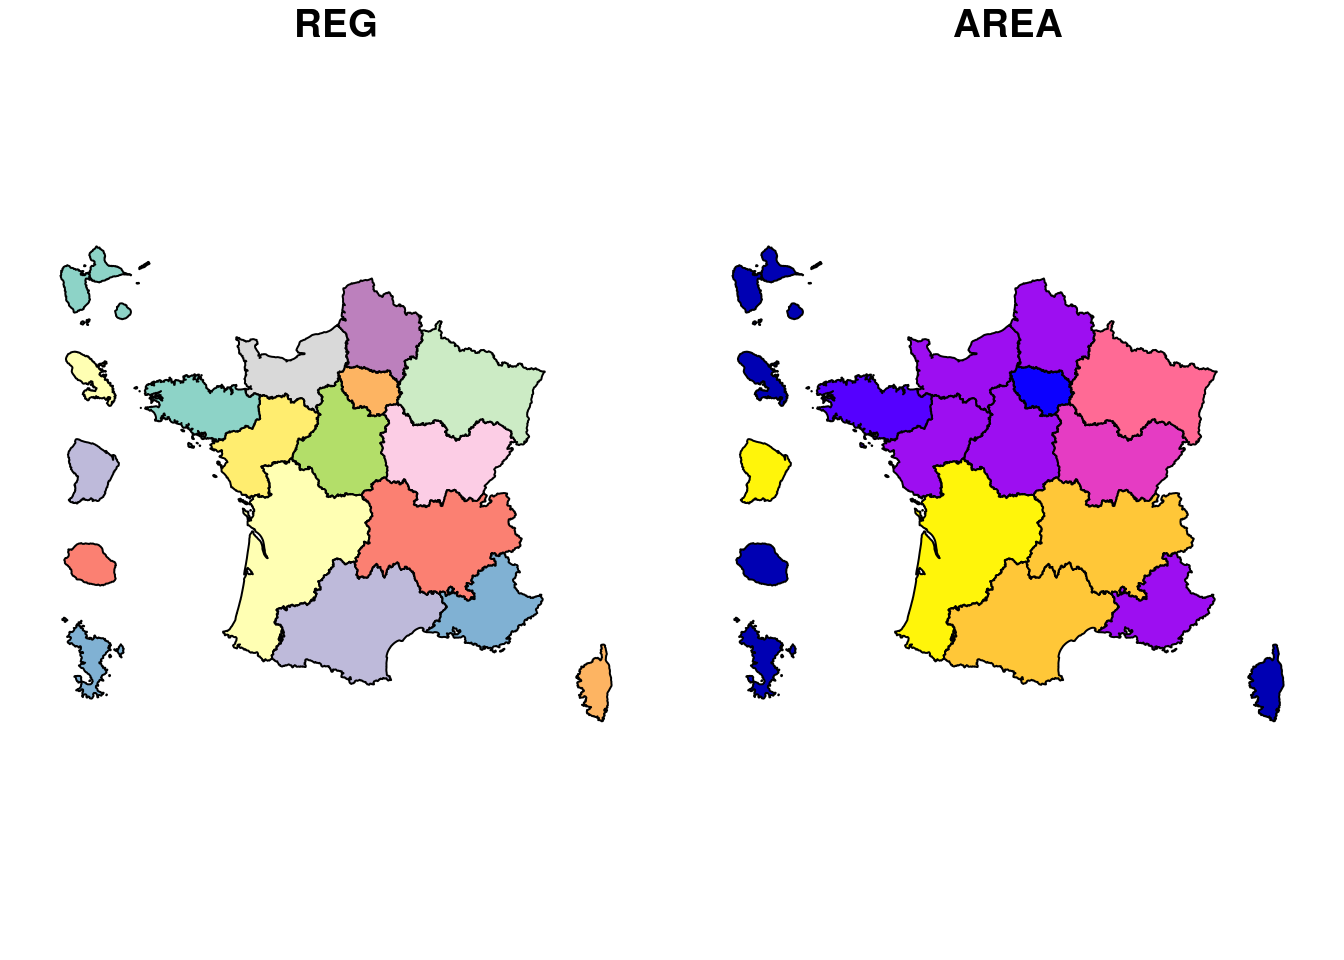
\includegraphics{support_m7_files/figure-latex/unnamed-chunk-107-1.pdf}

La fonction \texttt{annotate()} permet aussi d'ajouter d'autres types d'annotation comme par exemple des rectangles:

\begin{Shaded}
\begin{Highlighting}[]
\NormalTok{sdg\_indicators }\SpecialCharTok{\%\textgreater{}\%} 
  \FunctionTok{filter}\NormalTok{(timeperiod }\SpecialCharTok{==}\DecValTok{2015}\NormalTok{) }\SpecialCharTok{\%\textgreater{}\%} 
  \FunctionTok{ggplot}\NormalTok{() }\SpecialCharTok{+}
  \FunctionTok{geom\_point}\NormalTok{(}\FunctionTok{aes}\NormalTok{(}\AttributeTok{x =}\NormalTok{ gdp\_per\_cap, }
                 \AttributeTok{y =}\NormalTok{ sh\_sta\_mmr,}
                 \AttributeTok{color =}\NormalTok{ continent),}
    \AttributeTok{alpha =} \FloatTok{0.5}\NormalTok{, }
    \AttributeTok{size =} \FloatTok{1.9}
\NormalTok{  ) }\SpecialCharTok{+}
  \FunctionTok{labs}\NormalTok{(}
    \AttributeTok{title =} \StringTok{"Mortalité maternelle en fonction du PIB par habitant"}\NormalTok{,}
    \AttributeTok{subtitle =} \StringTok{"En 2015"}\NormalTok{,}
    \AttributeTok{x =} \StringTok{"PIB par habitant"}\NormalTok{,}
    \AttributeTok{y =} \StringTok{"Taux de mortalité de la mère }\SpecialCharTok{\textbackslash{}n}\StringTok{(pour 100 000 naissances)"}\NormalTok{,}
    \AttributeTok{caption =} \StringTok{"Source : ODD / ONU"}
\NormalTok{  ) }\SpecialCharTok{+}
  \FunctionTok{annotate}\NormalTok{(}\StringTok{"rect"}\NormalTok{, }\AttributeTok{xmin =} \DecValTok{10}\NormalTok{, }\AttributeTok{xmax =} \ConstantTok{Inf}\NormalTok{, }\AttributeTok{ymin =} \SpecialCharTok{{-}}\ConstantTok{Inf}\NormalTok{, }\AttributeTok{ymax =} \ConstantTok{Inf}\NormalTok{, }\AttributeTok{fill =} \StringTok{"red"}\NormalTok{, }\AttributeTok{alpha =} \FloatTok{0.2}\NormalTok{) }\SpecialCharTok{+}
  \FunctionTok{annotate}\NormalTok{(}\StringTok{"rect"}\NormalTok{, }\AttributeTok{xmin =} \SpecialCharTok{{-}}\ConstantTok{Inf}\NormalTok{, }\AttributeTok{xmax =} \ConstantTok{Inf}\NormalTok{, }\AttributeTok{ymin =} \SpecialCharTok{{-}}\ConstantTok{Inf}\NormalTok{, }\AttributeTok{ymax =} \DecValTok{2}\NormalTok{, }\AttributeTok{fill =} \StringTok{"green"}\NormalTok{, }\AttributeTok{alpha =} \FloatTok{0.2}\NormalTok{)}
\end{Highlighting}
\end{Shaded}

\includegraphics{support_m7_files/figure-latex/unnamed-chunk-108-1.pdf}

\hypertarget{les-thuxe8mes}{%
\subsection{Les thèmes}\label{les-thuxe8mes}}

Pour modifier simplement la position de la légende, c'est la fonction \href{http://ggplot2.tidyverse.org/reference/theme.html}{\texttt{theme()}} qu'il faut utiliser.

\texttt{theme()} permet de créer des templates, c'est à dire de définir tout ce qui n'est pas lié directement aux données sur un graphique, notamment:

\begin{itemize}
\item
  la position, taille,couleur,police des éléments textuels
\item
  la couleur des grilles primaires et secondaires du graphique
\end{itemize}

Il existe des \href{http://ggplot2.tidyverse.org/reference/index.html\#section-themes}{thèmes prédéfinis} dans ggplot que l'on peut déjà utiliser.
Par exemple: \texttt{theme\_classic()}, \texttt{theme\_bw()}, \texttt{theme\_dark()}, \ldots{}

Des packages externes permettent d'enrichir cette collection de thèmes, par exemple \texttt{ggthemes} ou \texttt{hrbrthemes}.

Lorsque l'on souhaite garder une cohérence entre plusieurs graphiques, le mieux est d'en définir un à part pour l'appeler ensuite.

\hypertarget{les-fonctions-uxe9luxe9ment}{%
\subsubsection{Les fonctions ``élément''}\label{les-fonctions-uxe9luxe9ment}}

Elle utilise 4 types de fonctions:

\begin{itemize}
\tightlist
\item
  \texttt{element\_text()} : pour toutes les étiquettes
\end{itemize}

\begin{longtable}[]{@{}ll@{}}
\toprule
PARAMÈTRE & VALEUR \\
\midrule
\endhead
family & la famille de la police \\
face & le type de police (``plain,'' ``italic,'' ``bold,'' ``bold.italic'') \\
colour & couleur \\
size & taille en points \\
hjust & justification horizontale, dans {[}0, 1{]} \\
vjust & justification verticale, dans {[}0, 1{]} \\
angle & angle, dans {[}0, 360{]} \\
lineheight & hauteur de ligne (pour l'espacement entre les lignes) \\
\bottomrule
\end{longtable}

\begin{itemize}
\tightlist
\item
  \texttt{element\_rect()} : pour les fonds et les cadres,
\end{itemize}

\begin{longtable}[]{@{}
  >{\raggedright\arraybackslash}p{(\columnwidth - 2\tabcolsep) * \real{0.14}}
  >{\raggedright\arraybackslash}p{(\columnwidth - 2\tabcolsep) * \real{0.86}}@{}}
\toprule
\begin{minipage}[b]{\linewidth}\raggedright
PARAMÈTRE
\end{minipage} & \begin{minipage}[b]{\linewidth}\raggedright
VALEUR
\end{minipage} \\
\midrule
\endhead
fill & la couleur de remplissage \\
colour & la couleur de la bordure \\
size & la taille de la bordure \\
linetype & le type de ligne (``blank,'' ``solid,'' ``dashed,'' ``dotted,'' ``dotdash,'' ``longdash,'' ``twodash) \\
\bottomrule
\end{longtable}

\begin{itemize}
\tightlist
\item
  \texttt{element\_line()} : pour toutes les lignes tracées,
\end{itemize}

\begin{longtable}[]{@{}
  >{\raggedright\arraybackslash}p{(\columnwidth - 2\tabcolsep) * \real{0.14}}
  >{\raggedright\arraybackslash}p{(\columnwidth - 2\tabcolsep) * \real{0.86}}@{}}
\toprule
\begin{minipage}[b]{\linewidth}\raggedright
PARAMÈTRE
\end{minipage} & \begin{minipage}[b]{\linewidth}\raggedright
VALEUR
\end{minipage} \\
\midrule
\endhead
colour & la couleur de ligne \\
size & la taille \\
linetype & le type de ligne (``blank,'' ``solid,'' ``dashed,'' ``dotted,'' ``dotdash,''``longdash,'' ``twodash) \\
lineend & le type de fin de ligne (``round,'' ``butt'' ou ``square'') \\
\bottomrule
\end{longtable}

\begin{itemize}
\tightlist
\item
  \texttt{element\_blank()} : permet de ne rien dessiner.
\end{itemize}

\hypertarget{les-composantes}{%
\subsubsection{Les composantes}\label{les-composantes}}

Il s'agit des différents éléments modifiables dans le thème.
Par exemple:

\textbf{Axes}
axis.line, axis.text.x, axis.text.y, axis.ticks, axis.title.x, axis.title.y,\ldots{}

\textbf{Légende}
legend.background, legend.key, legend.text, legend.title,\ldots{}

\textbf{Fond de graphe}
panel.background, panel.border, panel.grid.major, panel.grid.minor,\ldots{}

etc

\hypertarget{quelques-exemples}{%
\subsubsection{Quelques exemples}\label{quelques-exemples}}

\begin{itemize}
\tightlist
\item
  Changer le fond du graphique \texttt{panel\_background()}
\end{itemize}

\begin{Shaded}
\begin{Highlighting}[]
\NormalTok{sdg\_indicators }\SpecialCharTok{\%\textgreater{}\%} 
  \FunctionTok{filter}\NormalTok{(timeperiod }\SpecialCharTok{==}\DecValTok{2015}\NormalTok{) }\SpecialCharTok{\%\textgreater{}\%} 
  \FunctionTok{ggplot}\NormalTok{() }\SpecialCharTok{+}
  \FunctionTok{geom\_point}\NormalTok{(}\FunctionTok{aes}\NormalTok{(}\AttributeTok{x =}\NormalTok{ gdp\_per\_cap, }
                 \AttributeTok{y =}\NormalTok{ sh\_sta\_mmr,}
                 \AttributeTok{color =}\NormalTok{ continent),}
    \AttributeTok{alpha =} \FloatTok{0.5}\NormalTok{, }
    \AttributeTok{size =} \FloatTok{1.9}
\NormalTok{  ) }\SpecialCharTok{+}
  \FunctionTok{labs}\NormalTok{(}
    \AttributeTok{title =} \StringTok{"Mortalité maternelle en fonction du PIB par habitant"}\NormalTok{,}
    \AttributeTok{subtitle =} \StringTok{"En 2015"}\NormalTok{,}
    \AttributeTok{x =} \StringTok{"PIB par habitant"}\NormalTok{,}
    \AttributeTok{y =} \StringTok{"Taux de mortalité de la mère }\SpecialCharTok{\textbackslash{}n}\StringTok{(pour 100 000 naissances)"}\NormalTok{,}
    \AttributeTok{caption =} \StringTok{"Source : ODD / ONU"}
\NormalTok{  ) }\SpecialCharTok{+}
  \FunctionTok{theme}\NormalTok{(}\AttributeTok{panel.background =} \FunctionTok{element\_rect}\NormalTok{(}\AttributeTok{fill =} \StringTok{"Lavender"}\NormalTok{, }\AttributeTok{colour =} \StringTok{"black"}\NormalTok{))}
\end{Highlighting}
\end{Shaded}

\includegraphics{support_m7_files/figure-latex/unnamed-chunk-109-1.pdf}

\begin{itemize}
\tightlist
\item
  Changer l'apparence du quadrillage : \texttt{panel\_background()}
\end{itemize}

\begin{Shaded}
\begin{Highlighting}[]
\NormalTok{sdg\_indicators }\SpecialCharTok{\%\textgreater{}\%} 
  \FunctionTok{filter}\NormalTok{(timeperiod }\SpecialCharTok{==}\DecValTok{2015}\NormalTok{) }\SpecialCharTok{\%\textgreater{}\%} 
  \FunctionTok{ggplot}\NormalTok{() }\SpecialCharTok{+}
  \FunctionTok{geom\_point}\NormalTok{(}\FunctionTok{aes}\NormalTok{(}\AttributeTok{x =}\NormalTok{ gdp\_per\_cap, }
                 \AttributeTok{y =}\NormalTok{ sh\_sta\_mmr,}
                 \AttributeTok{color =}\NormalTok{ continent),}
    \AttributeTok{alpha =} \FloatTok{0.5}\NormalTok{, }
    \AttributeTok{size =} \FloatTok{1.9}
\NormalTok{  ) }\SpecialCharTok{+}
  \FunctionTok{labs}\NormalTok{(}
    \AttributeTok{title =} \StringTok{"Mortalité maternelle en fonction du PIB par habitant"}\NormalTok{,}
    \AttributeTok{subtitle =} \StringTok{"En 2015"}\NormalTok{,}
    \AttributeTok{x =} \StringTok{"PIB par habitant"}\NormalTok{,}
    \AttributeTok{y =} \StringTok{"Taux de mortalité de la mère }\SpecialCharTok{\textbackslash{}n}\StringTok{(pour 100 000 naissances)"}\NormalTok{,}
    \AttributeTok{caption =} \StringTok{"Source : ODD / ONU"}
\NormalTok{  ) }\SpecialCharTok{+}
  \FunctionTok{theme}\NormalTok{(}\AttributeTok{panel.grid.major =} \FunctionTok{element\_line}\NormalTok{(}\AttributeTok{colour =} \StringTok{"gray"}\NormalTok{, }\AttributeTok{size =} \FloatTok{0.5}\NormalTok{, }\AttributeTok{linetype =} \StringTok{"dashed"}\NormalTok{))}
\end{Highlighting}
\end{Shaded}

\includegraphics{support_m7_files/figure-latex/unnamed-chunk-110-1.pdf}

\begin{itemize}
\tightlist
\item
  Changer l'apparence des étiquettes des axes : \texttt{axis\_xxx()}
\end{itemize}

\begin{Shaded}
\begin{Highlighting}[]
\NormalTok{sdg\_indicators }\SpecialCharTok{\%\textgreater{}\%} 
  \FunctionTok{filter}\NormalTok{(timeperiod }\SpecialCharTok{==}\DecValTok{2015}\NormalTok{) }\SpecialCharTok{\%\textgreater{}\%} 
  \FunctionTok{ggplot}\NormalTok{() }\SpecialCharTok{+}
  \FunctionTok{geom\_point}\NormalTok{(}\FunctionTok{aes}\NormalTok{(}\AttributeTok{x =}\NormalTok{ gdp\_per\_cap, }
                 \AttributeTok{y =}\NormalTok{ sh\_sta\_mmr,}
                 \AttributeTok{color =}\NormalTok{ continent),}
    \AttributeTok{alpha =} \FloatTok{0.5}\NormalTok{, }
    \AttributeTok{size =} \FloatTok{1.9}
\NormalTok{  ) }\SpecialCharTok{+}
  \FunctionTok{labs}\NormalTok{(}
    \AttributeTok{title =} \StringTok{"Mortalité maternelle en fonction du PIB par habitant"}\NormalTok{,}
    \AttributeTok{subtitle =} \StringTok{"En 2015"}\NormalTok{,}
    \AttributeTok{x =} \StringTok{"PIB par habitant"}\NormalTok{,}
    \AttributeTok{y =} \StringTok{"Taux de mortalité de la mère }\SpecialCharTok{\textbackslash{}n}\StringTok{(pour 100 000 naissances)"}\NormalTok{,}
    \AttributeTok{caption =} \StringTok{"Source : ODD / ONU"}
\NormalTok{  ) }\SpecialCharTok{+}
  \FunctionTok{theme}\NormalTok{(}
    \AttributeTok{axis.text.x =} \FunctionTok{element\_text}\NormalTok{(}\AttributeTok{colour =} \StringTok{"blue"}\NormalTok{, }\AttributeTok{angle =} \DecValTok{45}\NormalTok{),}
    \AttributeTok{axis.title =} \FunctionTok{element\_text}\NormalTok{(}\AttributeTok{face =} \StringTok{"bold"}\NormalTok{, }\AttributeTok{colour =} \StringTok{"orange"}\NormalTok{)}
\NormalTok{  )}
\end{Highlighting}
\end{Shaded}

\includegraphics{support_m7_files/figure-latex/unnamed-chunk-111-1.pdf}

Certains changements de paramètres ne nécessitent pas l'utilisation de fonctions \texttt{element\_()}.
Par exemple, pour changer la position de la légende : \texttt{legend.xxx()}

\begin{Shaded}
\begin{Highlighting}[]
\NormalTok{sdg\_indicators }\SpecialCharTok{\%\textgreater{}\%} 
  \FunctionTok{filter}\NormalTok{(timeperiod }\SpecialCharTok{==}\DecValTok{2015}\NormalTok{) }\SpecialCharTok{\%\textgreater{}\%} 
  \FunctionTok{ggplot}\NormalTok{() }\SpecialCharTok{+}
  \FunctionTok{geom\_point}\NormalTok{(}\FunctionTok{aes}\NormalTok{(}\AttributeTok{x =}\NormalTok{ gdp\_per\_cap, }
                 \AttributeTok{y =}\NormalTok{ sh\_sta\_mmr,}
                 \AttributeTok{color =}\NormalTok{ continent),}
    \AttributeTok{alpha =} \FloatTok{0.5}\NormalTok{, }
    \AttributeTok{size =} \FloatTok{1.9}
\NormalTok{  ) }\SpecialCharTok{+}
  \FunctionTok{labs}\NormalTok{(}
    \AttributeTok{title =} \StringTok{"Mortalité maternelle en fonction du PIB par habitant"}\NormalTok{,}
    \AttributeTok{subtitle =} \StringTok{"En 2015"}\NormalTok{,}
    \AttributeTok{x =} \StringTok{"PIB par habitant"}\NormalTok{,}
    \AttributeTok{y =} \StringTok{"Taux de mortalité de la mère }\SpecialCharTok{\textbackslash{}n}\StringTok{(pour 100 000 naissances)"}\NormalTok{,}
    \AttributeTok{caption =} \StringTok{"Source : ODD / ONU"}
\NormalTok{  ) }\SpecialCharTok{+}
  \FunctionTok{theme}\NormalTok{(}\AttributeTok{legend.position =} \StringTok{"left"}\NormalTok{, }\AttributeTok{legend.title =} \FunctionTok{element\_blank}\NormalTok{())}
\end{Highlighting}
\end{Shaded}

\includegraphics{support_m7_files/figure-latex/unnamed-chunk-112-1.pdf}

\hypertarget{modifier-le-thuxe8me-par-duxe9faut.}{%
\subsubsection{Modifier le thème par défaut.}\label{modifier-le-thuxe8me-par-duxe9faut.}}

La fonction \texttt{theme\_set()} vous permet de définir un thème par défaut pour l'ensemble de vos graphiques.

\begin{Shaded}
\begin{Highlighting}[]
\FunctionTok{theme\_set}\NormalTok{(}\FunctionTok{theme\_dark}\NormalTok{())}

\NormalTok{sdg\_indicators }\SpecialCharTok{\%\textgreater{}\%} 
  \FunctionTok{filter}\NormalTok{(timeperiod }\SpecialCharTok{==}\DecValTok{2015}\NormalTok{) }\SpecialCharTok{\%\textgreater{}\%} 
  \FunctionTok{ggplot}\NormalTok{() }\SpecialCharTok{+}
  \FunctionTok{geom\_point}\NormalTok{(}\FunctionTok{aes}\NormalTok{(}\AttributeTok{x =}\NormalTok{ gdp\_per\_cap, }
                 \AttributeTok{y =}\NormalTok{ sh\_sta\_mmr,}
                 \AttributeTok{color =}\NormalTok{ continent),}
    \AttributeTok{alpha =} \FloatTok{0.5}\NormalTok{, }
    \AttributeTok{size =} \FloatTok{1.9}
\NormalTok{  ) }\SpecialCharTok{+}
  \FunctionTok{labs}\NormalTok{(}
    \AttributeTok{title =} \StringTok{"Mortalité maternelle en fonction du PIB par habitant"}\NormalTok{,}
    \AttributeTok{subtitle =} \StringTok{"En 2015"}\NormalTok{,}
    \AttributeTok{x =} \StringTok{"PIB par habitant"}\NormalTok{,}
    \AttributeTok{y =} \StringTok{"Taux de mortalité de la mère }\SpecialCharTok{\textbackslash{}n}\StringTok{(pour 100 000 naissances)"}\NormalTok{,}
    \AttributeTok{caption =} \StringTok{"Source : ODD / ONU"}
\NormalTok{  )}
\end{Highlighting}
\end{Shaded}

\includegraphics{support_m7_files/figure-latex/unnamed-chunk-113-1.pdf}

\hypertarget{cruxe9er-son-propre-thuxe8me}{%
\subsubsection{Créer son propre thème}\label{cruxe9er-son-propre-thuxe8me}}

Un thème est une fonction R qui va prendre en paramètre des éléments que vous souhaitez pouvoir faire varier et fixer des éléments que vous souhaitez avoir comme rendu par défaut.

Créons ici un thème avec un fond vert pour le ministère de la transition écologique et solidaire. On rajoute un paramètre pour la taille de la police du titre du graphique.

\begin{Shaded}
\begin{Highlighting}[]
\NormalTok{theme\_mtes }\OtherTok{\textless{}{-}} \ControlFlowTok{function}\NormalTok{(}\AttributeTok{taille\_police =} \DecValTok{14}\NormalTok{) \{}
  \FunctionTok{theme\_bw}\NormalTok{() }\SpecialCharTok{+}
    \FunctionTok{theme}\NormalTok{(}
      \AttributeTok{plot.title =} \FunctionTok{element\_text}\NormalTok{(}\AttributeTok{color =} \StringTok{"white"}\NormalTok{, }\AttributeTok{size =}\NormalTok{ taille\_police, }\AttributeTok{face =} \StringTok{"bold"}\NormalTok{),}
      \AttributeTok{text =} \FunctionTok{element\_text}\NormalTok{(}\AttributeTok{color =} \StringTok{"white"}\NormalTok{),}
      \AttributeTok{axis.text =} \FunctionTok{element\_text}\NormalTok{(}\AttributeTok{color =} \StringTok{"white"}\NormalTok{),}
      \AttributeTok{panel.background =} \FunctionTok{element\_rect}\NormalTok{(}\AttributeTok{fill =} \StringTok{"lightgreen"}\NormalTok{, }\AttributeTok{colour =} \StringTok{"lightgreen"}\NormalTok{),}
      \AttributeTok{plot.background =} \FunctionTok{element\_rect}\NormalTok{(}\AttributeTok{fill =} \StringTok{"\#006400"}\NormalTok{, }\AttributeTok{colour =} \StringTok{"lightgreen"}\NormalTok{),}
      \AttributeTok{legend.background =} \FunctionTok{element\_rect}\NormalTok{(}\AttributeTok{fill =} \StringTok{"lightgreen"}\NormalTok{, }\AttributeTok{colour =} \StringTok{"lightgreen"}\NormalTok{),}
      \AttributeTok{legend.key =} \FunctionTok{element\_blank}\NormalTok{()}
\NormalTok{    )}
\NormalTok{\}}

\NormalTok{sdg\_indicators }\SpecialCharTok{\%\textgreater{}\%} 
  \FunctionTok{filter}\NormalTok{(timeperiod }\SpecialCharTok{==}\DecValTok{2015}\NormalTok{) }\SpecialCharTok{\%\textgreater{}\%} 
  \FunctionTok{ggplot}\NormalTok{() }\SpecialCharTok{+}
  \FunctionTok{geom\_point}\NormalTok{(}\FunctionTok{aes}\NormalTok{(}\AttributeTok{x =}\NormalTok{ gdp\_per\_cap, }
                 \AttributeTok{y =}\NormalTok{ sh\_sta\_mmr,}
                 \AttributeTok{color =}\NormalTok{ continent),}
    \AttributeTok{alpha =} \FloatTok{0.5}\NormalTok{, }
    \AttributeTok{size =} \FloatTok{1.9}
\NormalTok{  ) }\SpecialCharTok{+}
  \FunctionTok{labs}\NormalTok{(}
    \AttributeTok{title =} \StringTok{"Mortalité maternelle en fonction du PIB par habitant"}\NormalTok{,}
    \AttributeTok{subtitle =} \StringTok{"En 2015"}\NormalTok{,}
    \AttributeTok{x =} \StringTok{"PIB par habitant"}\NormalTok{,}
    \AttributeTok{y =} \StringTok{"Taux de mortalité de la mère }\SpecialCharTok{\textbackslash{}n}\StringTok{(pour 100 000 naissances)"}\NormalTok{,}
    \AttributeTok{caption =} \StringTok{"Source : ODD / ONU"}
\NormalTok{  ) }\SpecialCharTok{+}
  \FunctionTok{theme\_mtes}\NormalTok{()}
\end{Highlighting}
\end{Shaded}

\includegraphics{support_m7_files/figure-latex/unnamed-chunk-114-1.pdf}

\hypertarget{les-scales}{%
\subsection{Les scales}\label{les-scales}}

Les fonctions \texttt{scales()} permettent globalement de paramétrer les éléments rentrés dans l'aesthétic :

\begin{itemize}
\item
  Si je veux un gradient de couleurs fonction d'une variable continue : quelle palette de couleurs je choisie, comment je cale mon dégradé en fonction de cette variable continue ?
\item
  Si je met une variable continue en ordonnée, comment je définis le minimum et maximum de cette axe, sa position, les valeurs que j'affiche sur l'échelle\ldots{}
\end{itemize}

L'ensemble des scales possibles peuvent se décrire sous la forme suivante:

\texttt{scale\_xx\_yy()}

ou \texttt{xx} peut être un des paramètres de l'aesthétic :

\begin{longtable}[]{@{}ll@{}}
\toprule
xx & description \\
\midrule
\endhead
alpha & transparence \\
color & couleur des lignes ou des points \\
fill & couleurs des aires \\
linetype & type de ligne (continue,pointillée,\ldots) \\
shape & forme des points \\
size & aire des points \\
x & variable de l'axe x \\
y & variable de l'axe y \\
\bottomrule
\end{longtable}

Et \texttt{yy} un type de paramétrage :

\begin{longtable}[]{@{}
  >{\raggedright\arraybackslash}p{(\columnwidth - 2\tabcolsep) * \real{0.40}}
  >{\raggedright\arraybackslash}p{(\columnwidth - 2\tabcolsep) * \real{0.60}}@{}}
\toprule
\begin{minipage}[b]{\linewidth}\raggedright
yy
\end{minipage} & \begin{minipage}[b]{\linewidth}\raggedright
description
\end{minipage} \\
\midrule
\endhead
continuous & gérer les variables continue \\
discrete & gérer les variables discrètes \\
date & gérer une variable au format date \\
reverse & inverser l'axe \\
log & convertire l'échelle d'une variable continue en échelle logarithmique \\
log10 & convertire l'échelle d'une variable continue en échelle logarithmique décimale \\
viridis & utiliser une palette de couleur viridis \\
brewer & utiliser une palette de couleur brewer (variable discrète) \\
distiller & utiliser une palette de couleur brewer (variable continue) \\
gradient & utiliser un gradient de 2 couleurs \\
gradient2 & utiliser un gradient divergent de 3 couleurs \\
\bottomrule
\end{longtable}

\begin{Shaded}
\begin{Highlighting}[]
\NormalTok{sdg\_indicators }\SpecialCharTok{\%\textgreater{}\%} 
  \FunctionTok{filter}\NormalTok{(timeperiod }\SpecialCharTok{==}\DecValTok{2015}\NormalTok{) }\SpecialCharTok{\%\textgreater{}\%} 
  \FunctionTok{ggplot}\NormalTok{() }\SpecialCharTok{+}
  \FunctionTok{geom\_point}\NormalTok{(}\FunctionTok{aes}\NormalTok{(}\AttributeTok{x =}\NormalTok{ gdp\_per\_cap, }
                 \AttributeTok{y =}\NormalTok{ sh\_sta\_mmr,}
                 \AttributeTok{color =}\NormalTok{ continent),}
    \AttributeTok{alpha =} \FloatTok{0.5}\NormalTok{, }
    \AttributeTok{size =} \FloatTok{1.9}
\NormalTok{  ) }\SpecialCharTok{+}
  \FunctionTok{labs}\NormalTok{(}
    \AttributeTok{title =} \StringTok{"Mortalité maternelle en fonction du PIB par habitant"}\NormalTok{,}
    \AttributeTok{subtitle =} \StringTok{"En 2015"}\NormalTok{,}
    \AttributeTok{x =} \StringTok{"PIB par habitant"}\NormalTok{,}
    \AttributeTok{y =} \StringTok{"Taux de mortalité de la mère }\SpecialCharTok{\textbackslash{}n}\StringTok{(pour 100 000 naissances)"}\NormalTok{,}
    \AttributeTok{caption =} \StringTok{"Source : ODD / ONU"}
\NormalTok{  ) }\SpecialCharTok{+}
  \FunctionTok{scale\_color\_brewer}\NormalTok{(}\AttributeTok{type =} \StringTok{"qual"}\NormalTok{)}
\end{Highlighting}
\end{Shaded}

\includegraphics{support_m7_files/figure-latex/unnamed-chunk-115-1.pdf}

Par exemple on peut exploiter une fonction scale pour définir une échelle logarithimique sur un axe.

\begin{Shaded}
\begin{Highlighting}[]
\NormalTok{sdg\_indicators }\SpecialCharTok{\%\textgreater{}\%} 
  \FunctionTok{filter}\NormalTok{(timeperiod }\SpecialCharTok{==}\DecValTok{2015}\NormalTok{) }\SpecialCharTok{\%\textgreater{}\%} 
  \FunctionTok{ggplot}\NormalTok{() }\SpecialCharTok{+}
  \FunctionTok{geom\_point}\NormalTok{(}\FunctionTok{aes}\NormalTok{(}\AttributeTok{x =}\NormalTok{ gdp\_per\_cap, }
                 \AttributeTok{y =}\NormalTok{ sh\_sta\_mmr,}
                 \AttributeTok{color =}\NormalTok{ continent),}
    \AttributeTok{alpha =} \FloatTok{0.5}\NormalTok{, }
    \AttributeTok{size =} \FloatTok{1.9}
\NormalTok{  ) }\SpecialCharTok{+}
  \FunctionTok{labs}\NormalTok{(}
    \AttributeTok{title =} \StringTok{"Mortalité maternelle en fonction du PIB par habitant"}\NormalTok{,}
    \AttributeTok{subtitle =} \StringTok{"En 2015"}\NormalTok{,}
    \AttributeTok{x =} \StringTok{"PIB par habitant"}\NormalTok{,}
    \AttributeTok{y =} \StringTok{"Taux de mortalité de la mère }\SpecialCharTok{\textbackslash{}n}\StringTok{(pour 100 000 naissances)"}\NormalTok{,}
    \AttributeTok{caption =} \StringTok{"Source : ODD / ONU"}
\NormalTok{  ) }\SpecialCharTok{+}
  \FunctionTok{scale\_color\_brewer}\NormalTok{(}\AttributeTok{type =} \StringTok{"qual"}\NormalTok{) }\SpecialCharTok{+}
  \FunctionTok{scale\_x\_log10}\NormalTok{() }\SpecialCharTok{+}
  \FunctionTok{scale\_y\_log10}\NormalTok{()}
\end{Highlighting}
\end{Shaded}

\includegraphics{support_m7_files/figure-latex/unnamed-chunk-116-1.pdf}

\hypertarget{formatage-spuxe9cifique}{%
\subsubsection{Formatage spécifique}\label{formatage-spuxe9cifique}}

\begin{itemize}
\tightlist
\item
  Transformation en pourcentage;
\end{itemize}

\begin{Shaded}
\begin{Highlighting}[]
  \FunctionTok{scale\_y\_continuous}\NormalTok{(}\AttributeTok{labels =}\NormalTok{ scales}\SpecialCharTok{::}\NormalTok{percent)}
\end{Highlighting}
\end{Shaded}

\begin{itemize}
\tightlist
\item
  Ajout du séparateur des milliers;
\end{itemize}

\begin{Shaded}
\begin{Highlighting}[]
\FunctionTok{scale\_y\_continuous}\NormalTok{(}\AttributeTok{labels =} \ControlFlowTok{function}\NormalTok{(x) }\FunctionTok{format}\NormalTok{(x, }\AttributeTok{big.mark =} \StringTok{" "}\NormalTok{, }\AttributeTok{scientific =} \ConstantTok{FALSE}\NormalTok{))}
\end{Highlighting}
\end{Shaded}

\begin{itemize}
\tightlist
\item
  Ajout du symbole €;
\end{itemize}

\begin{Shaded}
\begin{Highlighting}[]
\FunctionTok{scale\_y\_continuous}\NormalTok{(}\AttributeTok{labels =} \ControlFlowTok{function}\NormalTok{(x) }\FunctionTok{paste}\NormalTok{(x, }\StringTok{" €"}\NormalTok{))}
\end{Highlighting}
\end{Shaded}

\hypertarget{la-mise-en-page-de-plusieurs-graphiques}{%
\subsection{La mise en page de plusieurs graphiques}\label{la-mise-en-page-de-plusieurs-graphiques}}

Le package \texttt{cowplot} permet la combinaison de plusieurs graphiques. Il est composé de plusieurs fonctions.

\begin{itemize}
\tightlist
\item
  le fonction \texttt{plot\_grid()} qui permet de disposer \textbf{\emph{n}} graphes sur \textbf{\emph{i}} colonnes et \textbf{\emph{j}} lignes
\end{itemize}

\begin{Shaded}
\begin{Highlighting}[]
\NormalTok{gg1 }\OtherTok{\textless{}{-}}\NormalTok{ sdg\_indicators }\SpecialCharTok{\%\textgreater{}\%} 
  \FunctionTok{filter}\NormalTok{(timeperiod }\SpecialCharTok{==}\DecValTok{2015}\NormalTok{) }\SpecialCharTok{\%\textgreater{}\%} 
  \FunctionTok{ggplot}\NormalTok{() }\SpecialCharTok{+}
  \FunctionTok{geom\_point}\NormalTok{(}\FunctionTok{aes}\NormalTok{(}\AttributeTok{x =}\NormalTok{ gdp\_per\_cap, }
                 \AttributeTok{y =}\NormalTok{ sh\_sta\_mmr,}
                 \AttributeTok{color =}\NormalTok{ continent),}
    \AttributeTok{alpha =} \FloatTok{0.5}\NormalTok{, }
    \AttributeTok{size =} \FloatTok{1.9}
\NormalTok{  ) }\SpecialCharTok{+}
  \FunctionTok{labs}\NormalTok{(}
    \AttributeTok{title =} \StringTok{"Mortalité maternelle en fonction du PIB par habitant"}\NormalTok{,}
    \AttributeTok{subtitle =} \StringTok{"En 2015"}\NormalTok{,}
    \AttributeTok{x =} \StringTok{"PIB par habitant"}\NormalTok{,}
    \AttributeTok{y =} \StringTok{"Taux de mortalité de la mère }\SpecialCharTok{\textbackslash{}n}\StringTok{(pour 100 000 naissances)"}\NormalTok{,}
    \AttributeTok{caption =} \StringTok{"Source : ODD / ONU"}
\NormalTok{  ) }\SpecialCharTok{+}
  \FunctionTok{scale\_x\_log10}\NormalTok{() }\SpecialCharTok{+}
  \FunctionTok{scale\_y\_log10}\NormalTok{() }\SpecialCharTok{+}
  \FunctionTok{theme}\NormalTok{(}\AttributeTok{axis.title =} \FunctionTok{element\_text}\NormalTok{(}\AttributeTok{size =} \DecValTok{9}\NormalTok{))}

\NormalTok{  gg2 }\OtherTok{\textless{}{-}}\NormalTok{ sdg\_indicators }\SpecialCharTok{\%\textgreater{}\%} 
    \FunctionTok{filter}\NormalTok{(timeperiod }\SpecialCharTok{==}\DecValTok{2015}\NormalTok{) }\SpecialCharTok{\%\textgreater{}\%} 
    \FunctionTok{ggplot}\NormalTok{()}\SpecialCharTok{+}
    \FunctionTok{geom\_density}\NormalTok{(}\FunctionTok{aes}\NormalTok{(}\AttributeTok{x=}\NormalTok{gdp\_per\_cap))}\SpecialCharTok{+}
    \FunctionTok{scale\_x\_log10}\NormalTok{()}

\FunctionTok{plot\_grid}\NormalTok{(gg1, gg2, }\AttributeTok{ncol =} \DecValTok{1}\NormalTok{, }\AttributeTok{nrow =} \DecValTok{2}\NormalTok{)}
\end{Highlighting}
\end{Shaded}

\includegraphics{support_m7_files/figure-latex/unnamed-chunk-120-1.pdf}

\begin{itemize}
\tightlist
\item
  la fonction \texttt{draw\_plot()} associée à \texttt{ggdraw()} qui permet de disposer les graphiques à des places spécifiques.
\end{itemize}

\texttt{ggdraw()} initialise le graphique

\begin{Shaded}
\begin{Highlighting}[]
\NormalTok{gg3 }\OtherTok{\textless{}{-}}\NormalTok{ sdg\_indicators }\SpecialCharTok{\%\textgreater{}\%} 
    \FunctionTok{filter}\NormalTok{(timeperiod }\SpecialCharTok{==} \DecValTok{2015}\NormalTok{) }\SpecialCharTok{\%\textgreater{}\%} 
    \FunctionTok{ggplot}\NormalTok{() }\SpecialCharTok{+}
    \FunctionTok{geom\_bar}\NormalTok{(}\FunctionTok{aes}\NormalTok{(}\AttributeTok{x =}\NormalTok{ continent, }\AttributeTok{fill =}\NormalTok{ continent)) }\SpecialCharTok{+}
  \FunctionTok{theme}\NormalTok{(}
    \AttributeTok{axis.title.x =} \FunctionTok{element\_blank}\NormalTok{(),}
    \AttributeTok{axis.text.x =} \FunctionTok{element\_blank}\NormalTok{()}
\NormalTok{  )}
\FunctionTok{ggdraw}\NormalTok{() }\SpecialCharTok{+}
  \FunctionTok{draw\_plot}\NormalTok{(gg1, }\AttributeTok{x =} \DecValTok{0}\NormalTok{, }\AttributeTok{y =}\NormalTok{ .}\DecValTok{5}\NormalTok{, }\AttributeTok{width =} \DecValTok{1}\NormalTok{, }\AttributeTok{height =}\NormalTok{ .}\DecValTok{5}\NormalTok{) }\SpecialCharTok{+}
  \FunctionTok{draw\_plot}\NormalTok{(gg2, }\AttributeTok{x =} \DecValTok{0}\NormalTok{, }\AttributeTok{y =} \DecValTok{0}\NormalTok{, }\AttributeTok{width =}\NormalTok{ .}\DecValTok{3}\NormalTok{, }\AttributeTok{height =}\NormalTok{ .}\DecValTok{5}\NormalTok{) }\SpecialCharTok{+}
  \FunctionTok{draw\_plot}\NormalTok{(gg3, }\AttributeTok{x =} \FloatTok{0.3}\NormalTok{, }\AttributeTok{y =} \DecValTok{0}\NormalTok{, }\AttributeTok{width =} \FloatTok{0.7}\NormalTok{, }\AttributeTok{height =}\NormalTok{ .}\DecValTok{5}\NormalTok{)}
\end{Highlighting}
\end{Shaded}

\includegraphics{support_m7_files/figure-latex/unnamed-chunk-121-1.pdf}

\hypertarget{les-facettes}{%
\subsection{Les facettes}\label{les-facettes}}

Lorsque l'on veut pouvoir réaliser un graphique pour plusieurs sous-ensembles, les facettes sont alors très utiles. On va ici l'illustrer avec la réalisation du même graphique ci-dessus mais pour plusieurs années différentes.

\begin{Shaded}
\begin{Highlighting}[]
\NormalTok{sdg\_indicators }\SpecialCharTok{\%\textgreater{}\%} 
  \FunctionTok{filter}\NormalTok{(timeperiod  }\SpecialCharTok{\%in\%} \FunctionTok{c}\NormalTok{(}\DecValTok{2000}\NormalTok{, }\DecValTok{2005}\NormalTok{, }\DecValTok{2010}\NormalTok{, }\DecValTok{2015}\NormalTok{),}
\NormalTok{         geoareaname }\SpecialCharTok{\%in\%} \FunctionTok{c}\NormalTok{(}\StringTok{"France"}\NormalTok{,}\StringTok{"Canada"}\NormalTok{,}\StringTok{"Burkina Faso"}\NormalTok{,}\StringTok{"China"}\NormalTok{,}\StringTok{"Australia"}\NormalTok{)) }\SpecialCharTok{\%\textgreater{}\%}
  \FunctionTok{ggplot}\NormalTok{() }\SpecialCharTok{+}
  \FunctionTok{geom\_bar}\NormalTok{(}\FunctionTok{aes}\NormalTok{(}\AttributeTok{x =}\NormalTok{ geoareaname, }\AttributeTok{weight =}\NormalTok{ sh\_sta\_mmr, }\AttributeTok{fill =}\NormalTok{ continent)) }\SpecialCharTok{+}
  \FunctionTok{theme\_minimal}\NormalTok{() }\SpecialCharTok{+}
  \FunctionTok{scale\_fill\_viridis\_d}\NormalTok{() }\SpecialCharTok{+}
  \FunctionTok{coord\_flip}\NormalTok{() }\SpecialCharTok{+}
  \FunctionTok{scale\_y\_log10}\NormalTok{()}\SpecialCharTok{+}
  \FunctionTok{labs}\NormalTok{(}
    \AttributeTok{title =} \StringTok{"Mortalité maternelle sur quelques pays"}\NormalTok{,}
    \AttributeTok{subtitle =} \StringTok{"En 2015"}\NormalTok{,}
    \AttributeTok{y =} \StringTok{"Taux de mortalité de la mère }\SpecialCharTok{\textbackslash{}n}\StringTok{(pour 100 000 naissances), échelle logarithmique"}\NormalTok{,}
    \AttributeTok{x =} \StringTok{"Pays"}\NormalTok{,}
    \AttributeTok{fill =} \StringTok{"Pays"}
\NormalTok{  ) }\SpecialCharTok{+}
  \FunctionTok{theme}\NormalTok{(}\AttributeTok{legend.position =} \StringTok{"none"}\NormalTok{) }\SpecialCharTok{+}
  \FunctionTok{facet\_wrap}\NormalTok{(}\SpecialCharTok{\textasciitilde{}}\NormalTok{timeperiod)}
\end{Highlighting}
\end{Shaded}

\includegraphics{support_m7_files/figure-latex/unnamed-chunk-122-1.pdf}

L'exemple pris ici ``scinde'' notre table en fonction d'une seule variable, mais on peut le faire sur plusieurs variables également.

On peut choisir avec \texttt{facet\_wrap()} :

\begin{itemize}
\tightlist
\item
  le nombre de colonnes ou de ligne sur lesquel on veut voir s'afficher le graphique
\item
  si on veut fixer l'échelle de l'un ou l'autre des axes ou les deux
\end{itemize}

\begin{Shaded}
\begin{Highlighting}[]
\NormalTok{sdg\_indicators }\SpecialCharTok{\%\textgreater{}\%} 
  \FunctionTok{filter}\NormalTok{(timeperiod  }\SpecialCharTok{\%in\%} \FunctionTok{c}\NormalTok{(}\DecValTok{2000}\NormalTok{, }\DecValTok{2005}\NormalTok{, }\DecValTok{2010}\NormalTok{, }\DecValTok{2015}\NormalTok{),}
\NormalTok{         geoareaname }\SpecialCharTok{\%in\%} \FunctionTok{c}\NormalTok{(}\StringTok{"France"}\NormalTok{,}\StringTok{"Canada"}\NormalTok{,}\StringTok{"Burkina Faso"}\NormalTok{,}\StringTok{"China"}\NormalTok{,}\StringTok{"Australia"}\NormalTok{)) }\SpecialCharTok{\%\textgreater{}\%}
  \FunctionTok{ggplot}\NormalTok{() }\SpecialCharTok{+}
  \FunctionTok{geom\_bar}\NormalTok{(}\FunctionTok{aes}\NormalTok{(}\AttributeTok{x =}\NormalTok{ geoareaname, }\AttributeTok{weight =}\NormalTok{ sh\_sta\_mmr, }\AttributeTok{fill =}\NormalTok{ continent)) }\SpecialCharTok{+}
  \FunctionTok{theme\_minimal}\NormalTok{() }\SpecialCharTok{+}
  \FunctionTok{scale\_fill\_viridis\_d}\NormalTok{() }\SpecialCharTok{+}
  \FunctionTok{coord\_flip}\NormalTok{() }\SpecialCharTok{+}
  \FunctionTok{scale\_y\_log10}\NormalTok{()}\SpecialCharTok{+}
  \FunctionTok{labs}\NormalTok{(}
    \AttributeTok{title =} \StringTok{"Mortalité maternelle sur quelques pays"}\NormalTok{,}
    \AttributeTok{subtitle =} \StringTok{"En 2015"}\NormalTok{,}
    \AttributeTok{y =} \StringTok{"Taux de mortalité de la mère }\SpecialCharTok{\textbackslash{}n}\StringTok{(pour 100 000 naissances), échelle logarithmique"}\NormalTok{,}
    \AttributeTok{x =} \StringTok{"Pays"}\NormalTok{,}
    \AttributeTok{fill =} \StringTok{"Pays"}
\NormalTok{  ) }\SpecialCharTok{+}
  \FunctionTok{theme}\NormalTok{(}\AttributeTok{legend.position =} \StringTok{"none"}\NormalTok{) }\SpecialCharTok{+}
  \FunctionTok{facet\_wrap}\NormalTok{(}\SpecialCharTok{\textasciitilde{}}\NormalTok{timeperiod, }\AttributeTok{ncol =} \DecValTok{4}\NormalTok{)}
\end{Highlighting}
\end{Shaded}

\includegraphics{support_m7_files/figure-latex/unnamed-chunk-123-1.pdf}

\hypertarget{exporter-un-graphique}{%
\subsection{Exporter un graphique}\label{exporter-un-graphique}}

ggplot contient une fonction \texttt{ggsave()} qui permet d'exporter nos graphiques au format image dans les formats suivants : eps, ps, tex (pictex), pdf, jpeg, tiff, png, bmp, svg or wmf

\begin{Shaded}
\begin{Highlighting}[]
\NormalTok{p }\OtherTok{\textless{}{-}}\NormalTok{ sdg\_indicators }\SpecialCharTok{\%\textgreater{}\%} 
  \FunctionTok{filter}\NormalTok{(timeperiod  }\SpecialCharTok{\%in\%} \FunctionTok{c}\NormalTok{(}\DecValTok{2000}\NormalTok{, }\DecValTok{2005}\NormalTok{, }\DecValTok{2010}\NormalTok{, }\DecValTok{2015}\NormalTok{),}
\NormalTok{         geoareaname }\SpecialCharTok{\%in\%} \FunctionTok{c}\NormalTok{(}\StringTok{"France"}\NormalTok{,}\StringTok{"Canada"}\NormalTok{,}\StringTok{"Burkina Faso"}\NormalTok{,}\StringTok{"China"}\NormalTok{,}\StringTok{"Australia"}\NormalTok{)) }\SpecialCharTok{\%\textgreater{}\%}
  \FunctionTok{ggplot}\NormalTok{() }\SpecialCharTok{+}
  \FunctionTok{geom\_bar}\NormalTok{(}\FunctionTok{aes}\NormalTok{(}\AttributeTok{x =}\NormalTok{ geoareaname, }\AttributeTok{weight =}\NormalTok{ sh\_sta\_mmr, }\AttributeTok{fill =}\NormalTok{ continent)) }\SpecialCharTok{+}
  \FunctionTok{theme\_minimal}\NormalTok{() }\SpecialCharTok{+}
  \FunctionTok{scale\_fill\_viridis\_d}\NormalTok{() }\SpecialCharTok{+}
  \FunctionTok{coord\_flip}\NormalTok{() }\SpecialCharTok{+}
  \FunctionTok{scale\_y\_log10}\NormalTok{()}\SpecialCharTok{+}
  \FunctionTok{labs}\NormalTok{(}
    \AttributeTok{title =} \StringTok{"Mortalité maternelle sur quelques pays"}\NormalTok{,}
    \AttributeTok{subtitle =} \StringTok{"En 2015"}\NormalTok{,}
    \AttributeTok{y =} \StringTok{"Taux de mortalité de la mère }\SpecialCharTok{\textbackslash{}n}\StringTok{(pour 100 000 naissances), échelle logarithmique"}\NormalTok{,}
    \AttributeTok{x =} \StringTok{"Pays"}\NormalTok{,}
    \AttributeTok{fill =} \StringTok{"Pays"}
\NormalTok{  ) }\SpecialCharTok{+}
  \FunctionTok{theme}\NormalTok{(}\AttributeTok{legend.position =} \StringTok{"none"}\NormalTok{) }\SpecialCharTok{+}
  \FunctionTok{facet\_wrap}\NormalTok{(}\SpecialCharTok{\textasciitilde{}}\NormalTok{timeperiod, }\AttributeTok{ncol =} \DecValTok{4}\NormalTok{)}

\FunctionTok{ggsave}\NormalTok{(}\StringTok{"figures/Mortalité maternelle sur quelques pays du globe.svg"}\NormalTok{, p, }\AttributeTok{width =} \DecValTok{12}\NormalTok{, }\AttributeTok{height =} \DecValTok{5}\NormalTok{)}
\end{Highlighting}
\end{Shaded}

\hypertarget{faire-des-cartes-avec-ggplot2}{%
\section{Faire des cartes avec ggplot2}\label{faire-des-cartes-avec-ggplot2}}

\hypertarget{les-cartes-choropluxe8the}{%
\subsection{Les cartes choroplèthe}\label{les-cartes-choropluxe8the}}

ggplot2 intègre une fonction geom permettant l'utilisation de données géomatrique : \texttt{geom\_sf()}

Celle ci doit se coupler avec la fonction \texttt{coord\_sf()} qui permet de s'assurer en cas de superposition de couches que celles-ci utiliseront bien le même crs en spécifiant le datum. \texttt{coord\_sf()} permet également de \emph{zoomer} sur la carte en spécifiant les bornes x et y de la carte, ou également de définir les labels des axes.

Le premier exemple que nous allons pouvoir voir, c'est une carte choroplèthe.

Pour cela, préalablement, nous allons intégrer à nos données un fond de carte : le \emph{spatial dataframe} \texttt{World} présent dans le package \texttt{tmap}

\begin{Shaded}
\begin{Highlighting}[]
\FunctionTok{data}\NormalTok{(}\StringTok{"World"}\NormalTok{)}

\NormalTok{sdg\_indicators\_sf }\OtherTok{\textless{}{-}}\NormalTok{ World }\SpecialCharTok{\%\textgreater{}\%}
  \FunctionTok{left\_join}\NormalTok{(sdg\_indicators) }\SpecialCharTok{\%\textgreater{}\%}
  \FunctionTok{st\_transform}\NormalTok{(}\AttributeTok{crs =} \FunctionTok{st\_crs}\NormalTok{(}\DecValTok{3857}\NormalTok{))}
\end{Highlighting}
\end{Shaded}

\begin{Shaded}
\begin{Highlighting}[]
\NormalTok{map\_sdg\_indicators }\OtherTok{\textless{}{-}}\NormalTok{ sdg\_indicators\_sf }\SpecialCharTok{\%\textgreater{}\%} 
  \FunctionTok{filter}\NormalTok{(timeperiod }\SpecialCharTok{==} \StringTok{"2015"}\NormalTok{) }\SpecialCharTok{\%\textgreater{}\%} 
  \FunctionTok{ggplot}\NormalTok{() }\SpecialCharTok{+}
  \FunctionTok{geom\_sf}\NormalTok{(}\FunctionTok{aes}\NormalTok{(}\AttributeTok{fill =} \FunctionTok{log}\NormalTok{(sh\_sta\_mmr)),}\AttributeTok{color=}\StringTok{"white"}\NormalTok{,}\AttributeTok{size=}\NormalTok{.}\DecValTok{2}\NormalTok{)}\SpecialCharTok{+}
  \FunctionTok{scale\_fill\_viridis\_c}\NormalTok{()}\SpecialCharTok{+}
  \FunctionTok{theme\_minimal}\NormalTok{()}\SpecialCharTok{+}
  \FunctionTok{theme}\NormalTok{(}\AttributeTok{panel.background =} \FunctionTok{element\_rect}\NormalTok{(}\AttributeTok{fill =} \StringTok{"light blue"}\NormalTok{))}
\NormalTok{map\_sdg\_indicators}
\end{Highlighting}
\end{Shaded}

\includegraphics{support_m7_files/figure-latex/unnamed-chunk-126-1.pdf}

On peut exploiter de la même façon les différentes fonctions vues précédement. Par exemple avec un peu de thème et de facet.

\begin{Shaded}
\begin{Highlighting}[]
\NormalTok{sdg\_indicators\_sf }\SpecialCharTok{\%\textgreater{}\%} 
  \FunctionTok{filter}\NormalTok{(timeperiod }\SpecialCharTok{\%in\%} \FunctionTok{c}\NormalTok{(}\StringTok{"2000"}\NormalTok{,}\StringTok{"2005"}\NormalTok{,}\StringTok{"2010"}\NormalTok{,}\StringTok{"2015"}\NormalTok{)) }\SpecialCharTok{\%\textgreater{}\%} 
           \FunctionTok{ggplot}\NormalTok{() }\SpecialCharTok{+}
           \FunctionTok{geom\_sf}\NormalTok{(}\FunctionTok{aes}\NormalTok{(}\AttributeTok{fill =} \FunctionTok{log}\NormalTok{(sh\_sta\_mmr)),}\AttributeTok{color=}\StringTok{"white"}\NormalTok{,}\AttributeTok{size=}\NormalTok{.}\DecValTok{2}\NormalTok{)}\SpecialCharTok{+}
           \FunctionTok{scale\_fill\_viridis\_c}\NormalTok{(}
             \AttributeTok{option =} \StringTok{"magma"}\NormalTok{,}
             \AttributeTok{direction =} \DecValTok{1}\NormalTok{,}
             \AttributeTok{breaks =} \FunctionTok{c}\NormalTok{(}\DecValTok{0}\NormalTok{, }\DecValTok{1}\NormalTok{, }\DecValTok{2}\NormalTok{, }\DecValTok{3}\NormalTok{, }\DecValTok{4}\NormalTok{, }\DecValTok{5}\NormalTok{, }\DecValTok{6}\NormalTok{, }\DecValTok{7}\NormalTok{))}\SpecialCharTok{+}
           \FunctionTok{guides}\NormalTok{(}
             \AttributeTok{colour =}\NormalTok{ F,}
             \AttributeTok{order =} \DecValTok{0}\NormalTok{,}
             \AttributeTok{fill =} \FunctionTok{guide\_legend}\NormalTok{(}
               \AttributeTok{direction =} \StringTok{"horizontal"}\NormalTok{,}
               \AttributeTok{keyheight =} \FunctionTok{unit}\NormalTok{(}\DecValTok{2}\NormalTok{, }\AttributeTok{units =} \StringTok{"mm"}\NormalTok{),}
               \AttributeTok{keywidth =} \FunctionTok{unit}\NormalTok{(}\DecValTok{20}\NormalTok{, }\AttributeTok{units =} \StringTok{"mm"}\NormalTok{),}
               \AttributeTok{order =} \DecValTok{1}\NormalTok{,}
               \AttributeTok{title.position =} \StringTok{"top"}\NormalTok{,}
               \AttributeTok{title.hjust =} \FloatTok{0.5}\NormalTok{,}
               \AttributeTok{nrow =} \DecValTok{1}\NormalTok{,}
               \AttributeTok{label.position =} \StringTok{"bottom"}\NormalTok{,}
               \AttributeTok{label.hjust =} \DecValTok{1}
\NormalTok{             )}
\NormalTok{           ) }\SpecialCharTok{+}
           \FunctionTok{theme\_minimal}\NormalTok{()}\SpecialCharTok{+}
           \FunctionTok{theme}\NormalTok{(}\AttributeTok{legend.position =} \StringTok{"bottom"}\NormalTok{,}
                 \AttributeTok{panel.background =} \FunctionTok{element\_rect}\NormalTok{(}\AttributeTok{fill =} \StringTok{"light blue"}\NormalTok{))}\SpecialCharTok{+}
           \FunctionTok{labs}\NormalTok{(}\AttributeTok{fill =} \StringTok{"Taux de mortalité infantile (échelle logarithmique)"}\NormalTok{) }\SpecialCharTok{+}
           \FunctionTok{facet\_wrap}\NormalTok{(}\SpecialCharTok{\textasciitilde{}}\NormalTok{timeperiod, }\AttributeTok{drop =}\NormalTok{ T)}
\end{Highlighting}
\end{Shaded}

\includegraphics{support_m7_files/figure-latex/unnamed-chunk-127-1.pdf}

\hypertarget{les-cartes-uxe0-ronds-proportionnels}{%
\subsection{Les cartes à ronds proportionnels}\label{les-cartes-uxe0-ronds-proportionnels}}

ggplot ne peut attribuer par défaut un rond proportionnel à un polygone.

Pour travailler sur des ronds proportionnels, il faut d'abord créer le centroid de nos zones et ensuite tracer un rond proportionnel avec \texttt{geom\_sf()}.

\begin{Shaded}
\begin{Highlighting}[]
\NormalTok{World\_centroid }\OtherTok{\textless{}{-}} \FunctionTok{st\_centroid}\NormalTok{(World, }\AttributeTok{of\_largest\_polygon =}\NormalTok{ T)}
\NormalTok{sdg\_indicators\_sf\_centroid }\OtherTok{\textless{}{-}}\NormalTok{ World\_centroid }\SpecialCharTok{\%\textgreater{}\%}
  \FunctionTok{left\_join}\NormalTok{(sdg\_indicators)}

\NormalTok{map\_sdg\_indicators\_centroid }\OtherTok{\textless{}{-}}\NormalTok{ sdg\_indicators\_sf\_centroid }\SpecialCharTok{\%\textgreater{}\%} 
  \FunctionTok{filter}\NormalTok{(timeperiod }\SpecialCharTok{==} \StringTok{"2015"}\NormalTok{,}\SpecialCharTok{!}\FunctionTok{is.na}\NormalTok{(sh\_sta\_mmr)) }\SpecialCharTok{\%\textgreater{}\%} 
  \FunctionTok{ggplot}\NormalTok{() }\SpecialCharTok{+}
  \FunctionTok{geom\_sf}\NormalTok{(}\AttributeTok{data =}\NormalTok{ World, }\AttributeTok{fill =} \StringTok{"white"}\NormalTok{) }\SpecialCharTok{+}
  \FunctionTok{geom\_sf}\NormalTok{(}\FunctionTok{aes}\NormalTok{(}\AttributeTok{color =}\NormalTok{ sh\_sta\_mmr, }\AttributeTok{size =}\NormalTok{ sh\_sta\_mmr))}\SpecialCharTok{+}
  \FunctionTok{theme\_minimal}\NormalTok{()}\SpecialCharTok{+}
  \FunctionTok{theme}\NormalTok{(}\AttributeTok{panel.background =} \FunctionTok{element\_rect}\NormalTok{(}\AttributeTok{fill =} \StringTok{"light blue"}\NormalTok{))}

\NormalTok{map\_sdg\_indicators\_centroid}
\end{Highlighting}
\end{Shaded}

\includegraphics{support_m7_files/figure-latex/unnamed-chunk-128-1.pdf}

\hypertarget{ajouter-une-barre-duxe9chelle-et-la-fluxe8che-du-nord}{%
\subsection{Ajouter une barre d'échelle et la flèche du nord}\label{ajouter-une-barre-duxe9chelle-et-la-fluxe8che-du-nord}}

Le package \texttt{ggspatial} permet d'enrichir simplement nos cartes \texttt{ggplot2} avec une barre d'échelle et la flèche du nord.

Les deux fonctions qui permettent cela sont \texttt{annotation\_scale()} et \texttt{annotation\_north\_arrow()}.

L'utilisation de ces fonctions nécessitent un système de coordonnées géographiques.

\begin{Shaded}
\begin{Highlighting}[]
\NormalTok{sdg\_indicators\_sf }\SpecialCharTok{\%\textgreater{}\%}
  \FunctionTok{filter}\NormalTok{(timeperiod }\SpecialCharTok{==} \StringTok{"2015"}\NormalTok{) }\SpecialCharTok{\%\textgreater{}\%}
  \FunctionTok{st\_transform}\NormalTok{(}\AttributeTok{crs =} \DecValTok{4326}\NormalTok{) }\SpecialCharTok{\%\textgreater{}\%}
  \FunctionTok{ggplot}\NormalTok{() }\SpecialCharTok{+}
  \FunctionTok{geom\_sf}\NormalTok{(}\FunctionTok{aes}\NormalTok{(}\AttributeTok{fill =} \FunctionTok{log}\NormalTok{(sh\_sta\_mmr)), }\AttributeTok{color =} \StringTok{"white"}\NormalTok{, }\AttributeTok{size =}\NormalTok{ .}\DecValTok{2}\NormalTok{) }\SpecialCharTok{+}
  \FunctionTok{coord\_sf}\NormalTok{(}\AttributeTok{crs =} \DecValTok{4326}\NormalTok{) }\SpecialCharTok{+}
  \FunctionTok{scale\_fill\_viridis\_c}\NormalTok{() }\SpecialCharTok{+}
  \FunctionTok{theme\_minimal}\NormalTok{() }\SpecialCharTok{+}
  \FunctionTok{theme}\NormalTok{(}\AttributeTok{panel.background =} \FunctionTok{element\_rect}\NormalTok{(}\AttributeTok{fill =} \StringTok{"light blue"}\NormalTok{)) }\SpecialCharTok{+}
  \FunctionTok{annotation\_scale}\NormalTok{(}\AttributeTok{location =} \StringTok{"br"}\NormalTok{, }\AttributeTok{line\_width =}\NormalTok{ .}\DecValTok{5}\NormalTok{) }\SpecialCharTok{+}
  \FunctionTok{annotation\_north\_arrow}\NormalTok{(}\AttributeTok{location =} \StringTok{"bl"}\NormalTok{, }\AttributeTok{height =} \FunctionTok{unit}\NormalTok{(}\FloatTok{0.7}\NormalTok{, }\StringTok{"cm"}\NormalTok{), }\AttributeTok{width =} \FunctionTok{unit}\NormalTok{(}\FloatTok{0.7}\NormalTok{, }\StringTok{"cm"}\NormalTok{))}
\end{Highlighting}
\end{Shaded}

\includegraphics{support_m7_files/figure-latex/unnamed-chunk-129-1.pdf}

\hypertarget{mettre-plusieurs-cartes-cuxf4te-uxe0-cuxf4te}{%
\subsection{Mettre plusieurs cartes côte à côte}\label{mettre-plusieurs-cartes-cuxf4te-uxe0-cuxf4te}}

On peut a partir d'une même carte vouloir réaliser un zoom sur une sous partie de celle-ci.
\texttt{coord\_sf()} va nous permettre de \emph{zoomer} sur une carte, et \texttt{cow\_plot()} va nous permettre d'afficher nos deux cartes côte à côte.

Pour zoomer sur une carte,\texttt{coord\_sf()} va avoir besoin des coordonnées \emph{x} et \emph{y} du cadre sur lequel on veut zoomer.
Le plus simple pour cela est de filtrer préalablement
notre spatial dataframe et de récupérer la bbox de celle-ci.

Filtrons par exemple sur le continent africain.

\begin{Shaded}
\begin{Highlighting}[]
\NormalTok{bbox\_africa }\OtherTok{\textless{}{-}}\NormalTok{ World }\SpecialCharTok{\%\textgreater{}\%} 
  \FunctionTok{filter}\NormalTok{(continent}\SpecialCharTok{==}\StringTok{"Africa"}\NormalTok{) }\SpecialCharTok{\%\textgreater{}\%} 
  \FunctionTok{st\_bbox}\NormalTok{()}
\end{Highlighting}
\end{Shaded}

On peut ensuite réaliser une carte zoomée sur l'Afrique.

\begin{Shaded}
\begin{Highlighting}[]
\NormalTok{map\_sdg\_indicators\_africa }\OtherTok{\textless{}{-}}\NormalTok{ sdg\_indicators\_sf }\SpecialCharTok{\%\textgreater{}\%}
  \FunctionTok{filter}\NormalTok{(timeperiod }\SpecialCharTok{==} \StringTok{"2015"}\NormalTok{) }\SpecialCharTok{\%\textgreater{}\%}
  \FunctionTok{ggplot}\NormalTok{() }\SpecialCharTok{+}
  \FunctionTok{geom\_sf}\NormalTok{(}\FunctionTok{aes}\NormalTok{(}\AttributeTok{fill =} \FunctionTok{log}\NormalTok{(sh\_sta\_mmr)), }\AttributeTok{color =} \StringTok{"white"}\NormalTok{, }\AttributeTok{size =}\NormalTok{ .}\DecValTok{2}\NormalTok{) }\SpecialCharTok{+}
  \FunctionTok{coord\_sf}\NormalTok{(}\AttributeTok{xlim =} \FunctionTok{c}\NormalTok{(bbox\_africa[}\DecValTok{1}\NormalTok{],bbox\_africa[}\DecValTok{3}\NormalTok{]),}
           \AttributeTok{ylim =} \FunctionTok{c}\NormalTok{(bbox\_africa[}\DecValTok{2}\NormalTok{],bbox\_africa[}\DecValTok{4}\NormalTok{])}
\NormalTok{           ) }\SpecialCharTok{+}
  \FunctionTok{scale\_fill\_viridis\_c}\NormalTok{() }\SpecialCharTok{+}
  \FunctionTok{theme\_minimal}\NormalTok{() }\SpecialCharTok{+}
  \FunctionTok{theme}\NormalTok{(}\AttributeTok{legend.position =} \StringTok{"right"}\NormalTok{, }\AttributeTok{panel.background =} \FunctionTok{element\_rect}\NormalTok{(}\AttributeTok{fill =} \StringTok{"light blue"}\NormalTok{))}
\end{Highlighting}
\end{Shaded}

On peut utiliser ensuite \texttt{plot\_grid()} pour afficher nos cartes côte à côte. Il faut jouer sur les largeurs relatives pour que les deux cartes s'agencent bien.

\begin{Shaded}
\begin{Highlighting}[]
\NormalTok{map\_sdg\_indicators\_compo }\OtherTok{\textless{}{-}}\NormalTok{ map\_sdg\_indicators }\SpecialCharTok{+}
  \FunctionTok{theme\_void}\NormalTok{()}\SpecialCharTok{+}
  \FunctionTok{theme}\NormalTok{(}\AttributeTok{panel.background =} \FunctionTok{element\_rect}\NormalTok{(}\AttributeTok{fill =} \StringTok{"light blue"}\NormalTok{),}\AttributeTok{legend.position =} \StringTok{"none"}\NormalTok{)}
\FunctionTok{plot\_grid}\NormalTok{(map\_sdg\_indicators\_compo,map\_sdg\_indicators\_africa,}\AttributeTok{rel\_widths =} \FunctionTok{c}\NormalTok{(}\FloatTok{1.7}\NormalTok{, }\DecValTok{1}\NormalTok{))}
\end{Highlighting}
\end{Shaded}

\includegraphics{support_m7_files/figure-latex/unnamed-chunk-132-1.pdf}

\hypertarget{cruxe9er-des-cartes-avec-tmap}{%
\chapter{Créer des cartes avec tmap}\label{cruxe9er-des-cartes-avec-tmap}}

\texttt{tmap} est un package dédié à la réalisation de cartes sous R.

La syntaxe est très proche de \texttt{ggplot}, avec l'opérateur \texttt{+} pour enchainer les options.

L'équivalent des \texttt{geom\_xx()} dans \texttt{tmap} sont les fonctions suivantes :

\begin{itemize}
\tightlist
\item
  \texttt{tm\_lines()} : afficher des lignes
\item
  \texttt{tm\_polygons()} : afficher des polygones
\item
  \texttt{tm\_raster()} : afficher un raster
\item
  \texttt{tm\_bubbles()} : afficher des ronds proportionnels
\item
  \texttt{tm\_markers()} : afficher des marqueurs
\item
  \texttt{tm\_text()} : afficher du texte
\end{itemize}

Les différences avec \texttt{ggplot2} :

\begin{itemize}
\tightlist
\item
  Les variables s'appellent dans des cotes \texttt{""} ;
\item
  Le facetting peut se faire sur un format de données large (une carte par colonne et non une carte par modalité d'une variable) ;
\item
  Les fonctions \texttt{tm\_xx()} incluent la définition des \emph{classes} (nombre de classe, définition des classes et des palettes) sans passer par une fonction \texttt{scale()} dont l'équivalent n'existe pas.
\end{itemize}

La mise en page se définit avec la fonction \texttt{tm\_layout()}, la légende avec \texttt{tm\_legend()}

Dans ce chapitre nous allons utiliser les packages suivants

\begin{Shaded}
\begin{Highlighting}[]
\FunctionTok{library}\NormalTok{(tmap)}
\FunctionTok{library}\NormalTok{(sf)}
\FunctionTok{library}\NormalTok{(tidyverse)}
\CommentTok{\#remotes::install\_github("MaelTheuliere/variousdata")}
\FunctionTok{library}\NormalTok{(variousdata)}
\end{Highlighting}
\end{Shaded}

\hypertarget{tm_shape}{%
\section{tm\_shape}\label{tm_shape}}

Pour charger une donnée géométrique, il faut utiliser la fonction \texttt{tm\_shape()}. \texttt{tm\_shape()} permet de fixer plusieurs options de base de notre carte : la projection, la bbox, un facteur de simplification\ldots{}

\begin{Shaded}
\begin{Highlighting}[]
\NormalTok{wgs\_84 }\OtherTok{\textless{}{-}} \FunctionTok{tm\_shape}\NormalTok{(World, }\AttributeTok{projection =} \FunctionTok{st\_crs}\NormalTok{(}\DecValTok{4326}\NormalTok{)) }\SpecialCharTok{+} 
    \FunctionTok{tm\_polygons}\NormalTok{() }\SpecialCharTok{+} 
\FunctionTok{tm\_layout}\NormalTok{(}\StringTok{"Le monde en projection WGS84"}\NormalTok{, }\AttributeTok{inner.margins=}\FunctionTok{c}\NormalTok{(}\DecValTok{0}\NormalTok{,}\DecValTok{0}\NormalTok{,.}\DecValTok{1}\NormalTok{,}\DecValTok{0}\NormalTok{), }\AttributeTok{title.size=}\NormalTok{.}\DecValTok{8}\NormalTok{)}

\NormalTok{robin }\OtherTok{\textless{}{-}} \FunctionTok{tm\_shape}\NormalTok{(World, }\AttributeTok{projection =} \FunctionTok{st\_crs}\NormalTok{(}\DecValTok{54042}\NormalTok{)) }\SpecialCharTok{+} 
    \FunctionTok{tm\_polygons}\NormalTok{() }\SpecialCharTok{+}
\FunctionTok{tm\_layout}\NormalTok{(}
\StringTok{"Le monde en project Winkel{-}Tripel"}\NormalTok{,}
    \AttributeTok{inner.margins=}\FunctionTok{c}\NormalTok{(}\DecValTok{0}\NormalTok{,}\DecValTok{0}\NormalTok{,.}\DecValTok{1}\NormalTok{,}\DecValTok{0}\NormalTok{), }\AttributeTok{title.size=}\NormalTok{.}\DecValTok{8}\NormalTok{)}
\end{Highlighting}
\end{Shaded}

\includegraphics{support_m7_files/figure-latex/unnamed-chunk-136-1.pdf}

\hypertarget{exemple-de-carte-choropluxe8the}{%
\section{Exemple de carte choroplèthe}\label{exemple-de-carte-choropluxe8the}}

La fonction \texttt{tm\_polygons()} permet de faire des cartes choroplèthe.

\begin{Shaded}
\begin{Highlighting}[]
\NormalTok{sdg\_indicators\_sf }\SpecialCharTok{\%\textgreater{}\%} 
  \FunctionTok{filter}\NormalTok{(timeperiod }\SpecialCharTok{==} \StringTok{"2015"}\NormalTok{) }\SpecialCharTok{\%\textgreater{}\%} 
  \FunctionTok{tm\_shape}\NormalTok{()}\SpecialCharTok{+}
  \FunctionTok{tm\_polygons}\NormalTok{(}\StringTok{"sh\_sta\_mmr"}\NormalTok{,}\AttributeTok{textNA=}\StringTok{"Valeur manquante"}\NormalTok{)}\SpecialCharTok{+}
  \FunctionTok{tm\_borders}\NormalTok{(}\StringTok{"white"}\NormalTok{, }\AttributeTok{lwd =}\NormalTok{ .}\DecValTok{5}\NormalTok{)}
\end{Highlighting}
\end{Shaded}

\includegraphics{support_m7_files/figure-latex/unnamed-chunk-137-1.pdf}

\hypertarget{exemple-de-carte-uxe0-ronds-proportionnels}{%
\section{Exemple de carte à ronds proportionnels}\label{exemple-de-carte-uxe0-ronds-proportionnels}}

La fonction \texttt{tm\_bubble()} permet de faire des cartes à ronds proportionnels. L'utilisation de \texttt{tm\_polygons()} permet sans lui spécifier de paramètre d'afficher les frontière des pays avec une couleur de remplissage par défaut.

\begin{Shaded}
\begin{Highlighting}[]
\NormalTok{sdg\_indicators\_sf }\SpecialCharTok{\%\textgreater{}\%} 
  \FunctionTok{filter}\NormalTok{(timeperiod }\SpecialCharTok{==} \StringTok{"2015"}\NormalTok{) }\SpecialCharTok{\%\textgreater{}\%} 
  \FunctionTok{tm\_shape}\NormalTok{()}\SpecialCharTok{+}
  \FunctionTok{tm\_polygons}\NormalTok{()}\SpecialCharTok{+}
  \FunctionTok{tm\_bubbles}\NormalTok{(}\AttributeTok{size=}\StringTok{"sh\_sta\_mmr"}\NormalTok{,}\AttributeTok{col=}\StringTok{"sh\_sta\_mmr"}\NormalTok{,}\AttributeTok{textNA =} \StringTok{"Valeur manquante"}\NormalTok{)}
\end{Highlighting}
\end{Shaded}

\includegraphics{support_m7_files/figure-latex/unnamed-chunk-138-1.pdf}

\hypertarget{discretisation}{%
\section{Discretisation}\label{discretisation}}

Pour définir comment notre variable continue va être discrétisée, deux méthodes :

\begin{itemize}
\item
  discrétiser à la main et indiquer les valeurs limites dans l'option \texttt{breaks} de notre \texttt{tm\_xx}
\item
  utiliser l'option \texttt{style} des \texttt{tm\_xx} qui permettent de choisir un algorithme de discrétisation.
\end{itemize}

La méthode de jenks par exemple permet de maximiser la variance interclasse.

\begin{Shaded}
\begin{Highlighting}[]
\NormalTok{sdg\_indicators\_sf }\SpecialCharTok{\%\textgreater{}\%} 
  \FunctionTok{filter}\NormalTok{(timeperiod }\SpecialCharTok{==} \StringTok{"2015"}\NormalTok{) }\SpecialCharTok{\%\textgreater{}\%} 
  \FunctionTok{tm\_shape}\NormalTok{()}\SpecialCharTok{+}
  \FunctionTok{tm\_polygons}\NormalTok{(}\StringTok{"sh\_sta\_mmr"}\NormalTok{, }\AttributeTok{textNA=}\StringTok{"Valeur manquante"}\NormalTok{, }\AttributeTok{style=}\StringTok{"jenks"}\NormalTok{)}
\end{Highlighting}
\end{Shaded}

\includegraphics{support_m7_files/figure-latex/unnamed-chunk-139-1.pdf}

L'option \texttt{n=} permet d'imposer un nombre de classes à la méthode utilisée.

\begin{Shaded}
\begin{Highlighting}[]
\NormalTok{sdg\_indicators\_sf }\SpecialCharTok{\%\textgreater{}\%} 
  \FunctionTok{filter}\NormalTok{(timeperiod }\SpecialCharTok{==} \StringTok{"2015"}\NormalTok{) }\SpecialCharTok{\%\textgreater{}\%} 
  \FunctionTok{tm\_shape}\NormalTok{()}\SpecialCharTok{+}
  \FunctionTok{tm\_polygons}\NormalTok{(}\StringTok{"sh\_sta\_mmr"}\NormalTok{, }\AttributeTok{textNA =} \StringTok{"Valeur manquante"}\NormalTok{, }\AttributeTok{style =} \StringTok{"jenks"}\NormalTok{,}\AttributeTok{n =} \DecValTok{3}\NormalTok{)}
\end{Highlighting}
\end{Shaded}

\includegraphics{support_m7_files/figure-latex/unnamed-chunk-140-1.pdf}

\hypertarget{exemples-de-cartes-avec-facet}{%
\section{Exemples de cartes avec facet}\label{exemples-de-cartes-avec-facet}}

\texttt{tm\_facets()} permet de réaliser des cartes à facette avec la même logique que celle de \texttt{ggplot2}.

\begin{Shaded}
\begin{Highlighting}[]
\NormalTok{sdg\_indicators\_sf }\SpecialCharTok{\%\textgreater{}\%}
  \FunctionTok{filter}\NormalTok{(timeperiod }\SpecialCharTok{\%in\%} \FunctionTok{c}\NormalTok{(}\StringTok{"2000"}\NormalTok{, }\StringTok{"2005"}\NormalTok{, }\StringTok{"2010"}\NormalTok{, }\StringTok{"2015"}\NormalTok{)) }\SpecialCharTok{\%\textgreater{}\%}
  \FunctionTok{tm\_shape}\NormalTok{() }\SpecialCharTok{+}
  \FunctionTok{tm\_polygons}\NormalTok{(}\StringTok{"sh\_sta\_mmr"}\NormalTok{, }\AttributeTok{textNA =} \StringTok{"Valeur manquante"}\NormalTok{, }\AttributeTok{style =} \StringTok{"jenks"}\NormalTok{) }\SpecialCharTok{+}
  \FunctionTok{tm\_facets}\NormalTok{(}\StringTok{"timeperiod"}\NormalTok{)}
\end{Highlighting}
\end{Shaded}

\includegraphics{support_m7_files/figure-latex/unnamed-chunk-141-1.pdf}

\hypertarget{gestion-des-palettes}{%
\section{gestion des palettes}\label{gestion-des-palettes}}

La fonction \texttt{tmaptools::palette\_explorer()} permet d'accéder à une interface très simple de définition d'une palette de couleur à partir des palette \emph{brewer}.

\begin{Shaded}
\begin{Highlighting}[]
\NormalTok{sdg\_indicators\_sf }\SpecialCharTok{\%\textgreater{}\%} 
  \FunctionTok{filter}\NormalTok{(timeperiod }\SpecialCharTok{==} \StringTok{"2015"}\NormalTok{) }\SpecialCharTok{\%\textgreater{}\%} 
  \FunctionTok{tm\_shape}\NormalTok{()}\SpecialCharTok{+}
  \FunctionTok{tm\_polygons}\NormalTok{(}\StringTok{"sh\_sta\_mmr"}\NormalTok{, }\AttributeTok{textNA =} \StringTok{"Valeur manquante"}\NormalTok{, }\AttributeTok{style =} \StringTok{"jenks"}\NormalTok{,}\AttributeTok{palette =} \FunctionTok{get\_brewer\_pal}\NormalTok{(}\StringTok{"OrRd"}\NormalTok{, }\AttributeTok{n =} \DecValTok{5}\NormalTok{, }\AttributeTok{contrast =} \FunctionTok{c}\NormalTok{(}\FloatTok{0.2}\NormalTok{, }\DecValTok{1}\NormalTok{)), }\AttributeTok{plot =}\NormalTok{ F)}
\end{Highlighting}
\end{Shaded}

\includegraphics{support_m7_files/figure-latex/unnamed-chunk-142-1.pdf} \includegraphics{support_m7_files/figure-latex/unnamed-chunk-142-2.pdf}

On peut également utiliser n'importe qu'elle palette, par exemple la pelette viridis, mais sans l'interface proposée par \texttt{palette\_explorer()} :

\begin{Shaded}
\begin{Highlighting}[]
\NormalTok{sdg\_indicators\_sf }\SpecialCharTok{\%\textgreater{}\%} 
  \FunctionTok{filter}\NormalTok{(timeperiod }\SpecialCharTok{==} \StringTok{"2015"}\NormalTok{) }\SpecialCharTok{\%\textgreater{}\%} 
  \FunctionTok{tm\_shape}\NormalTok{()}\SpecialCharTok{+}
  \FunctionTok{tm\_polygons}\NormalTok{(}\StringTok{"sh\_sta\_mmr"}\NormalTok{, }\AttributeTok{textNA =} \StringTok{"Valeur manquante"}\NormalTok{, }\AttributeTok{style =} \StringTok{"jenks"}\NormalTok{,}\AttributeTok{palette =} \FunctionTok{viridis}\NormalTok{(}\DecValTok{5}\NormalTok{, }\AttributeTok{alpha =} \DecValTok{1}\NormalTok{, }\AttributeTok{begin =} \FloatTok{0.3}\NormalTok{, }\AttributeTok{end =} \DecValTok{1}\NormalTok{, }\AttributeTok{direction =} \DecValTok{1}\NormalTok{, }\AttributeTok{option =} \StringTok{"D"}\NormalTok{))}
\end{Highlighting}
\end{Shaded}

\includegraphics{support_m7_files/figure-latex/unnamed-chunk-143-1.pdf}

\hypertarget{la-mise-en-page}{%
\section{La mise en page}\label{la-mise-en-page}}

\texttt{tm\_layout()} permet de controler les polices, la légende, les marges, les couleurs.
l'option \texttt{design.mode=T} permet de voir visuellement les marges,la position de la légende.
Le titre de la légende ne se définit pas dans \texttt{tm\_layout()} mais dans \texttt{tm\_polygons()}.

L'option \texttt{title} de ces fonctions est l'équivalent d'un libellé de la variable mise dans l'aesthetic.

On peut rajouter une barre d'échelle et la flèche du nord avec \texttt{tm\_scale\_bar()} et \texttt{tm\_compass()}.

\begin{Shaded}
\begin{Highlighting}[]
\NormalTok{sdg\_indicators\_sf }\SpecialCharTok{\%\textgreater{}\%} 
  \FunctionTok{filter}\NormalTok{(timeperiod }\SpecialCharTok{==} \StringTok{"2015"}\NormalTok{) }\SpecialCharTok{\%\textgreater{}\%} 
  \FunctionTok{tm\_shape}\NormalTok{()}\SpecialCharTok{+}
  \FunctionTok{tm\_polygons}\NormalTok{(}\StringTok{"sh\_sta\_mmr"}\NormalTok{,}\AttributeTok{textNA =} \StringTok{"Valeur manquante"}\NormalTok{, }\AttributeTok{style =} \StringTok{"jenks"}\NormalTok{,}\AttributeTok{palette =} \FunctionTok{viridis}\NormalTok{(}\DecValTok{5}\NormalTok{, }\AttributeTok{alpha =} \DecValTok{1}\NormalTok{, }\AttributeTok{begin =} \FloatTok{0.3}\NormalTok{, }\AttributeTok{end =} \DecValTok{1}\NormalTok{, }\AttributeTok{direction =} \DecValTok{1}\NormalTok{, }\AttributeTok{option =} \StringTok{"D"}\NormalTok{),}
              \AttributeTok{title =} \StringTok{"Taux de mortalité de la mère }\SpecialCharTok{\textbackslash{}n}\StringTok{(pour 100 000 naissances)"}\NormalTok{)}\SpecialCharTok{+}
  \FunctionTok{tm\_layout}\NormalTok{(}\AttributeTok{main.title =} \StringTok{"Taux de mortalité de la mère }\SpecialCharTok{\textbackslash{}n}\StringTok{(pour 100 000 naissances) dans le monde"}\NormalTok{,}
            \AttributeTok{main.title.size =} \FloatTok{1.2}\NormalTok{,}
            \AttributeTok{bg.color =} \StringTok{"skyblue"}\NormalTok{,}
            \AttributeTok{legend.position =} \FunctionTok{c}\NormalTok{(}\StringTok{"left"}\NormalTok{,}\StringTok{"bottom"}\NormalTok{),}
            \AttributeTok{legend.bg.color =} \StringTok{"white"}\NormalTok{,}
            \AttributeTok{legend.bg.alpha =}\NormalTok{ .}\DecValTok{4}\NormalTok{,}
            \AttributeTok{legend.outside =}\NormalTok{ F,}
            \AttributeTok{main.title.position =} \StringTok{"center"}\NormalTok{,}
            \AttributeTok{frame =} \ConstantTok{FALSE}\NormalTok{)}\SpecialCharTok{+}
  \FunctionTok{tm\_scale\_bar}\NormalTok{(}\AttributeTok{position =} \FunctionTok{c}\NormalTok{(}\StringTok{"center"}\NormalTok{,}\StringTok{"bottom"}\NormalTok{))}\SpecialCharTok{+}
  \FunctionTok{tm\_compass}\NormalTok{(}\AttributeTok{position =} \FunctionTok{c}\NormalTok{(}\StringTok{"right"}\NormalTok{,}\StringTok{"top"}\NormalTok{))}
\end{Highlighting}
\end{Shaded}

\includegraphics{support_m7_files/figure-latex/unnamed-chunk-144-1.pdf}

Avec les cartes en ronds proportionnels, on peut spécifier un titre pour la couleur et la taille du rond.

\begin{Shaded}
\begin{Highlighting}[]
\NormalTok{sdg\_indicators\_sf }\SpecialCharTok{\%\textgreater{}\%} 
  \FunctionTok{filter}\NormalTok{(timeperiod }\SpecialCharTok{==} \StringTok{"2015"}\NormalTok{) }\SpecialCharTok{\%\textgreater{}\%} 
  \FunctionTok{tm\_shape}\NormalTok{()}\SpecialCharTok{+}
  \FunctionTok{tm\_polygons}\NormalTok{()}\SpecialCharTok{+}
  \FunctionTok{tm\_bubbles}\NormalTok{(}\AttributeTok{size=}\StringTok{"sh\_sta\_mmr"}\NormalTok{,}\AttributeTok{col=}\StringTok{"sh\_sta\_mmr"}\NormalTok{,}\AttributeTok{style=}\StringTok{"jenks"}\NormalTok{,}
             \AttributeTok{palette=}\FunctionTok{viridis}\NormalTok{(}\DecValTok{5}\NormalTok{, }\AttributeTok{alpha =} \DecValTok{1}\NormalTok{, }\AttributeTok{begin =} \DecValTok{0}\NormalTok{, }\AttributeTok{end =} \DecValTok{1}\NormalTok{, }\AttributeTok{direction =} \DecValTok{1}\NormalTok{, }\AttributeTok{option =} \StringTok{"D"}\NormalTok{),}
              \AttributeTok{title.col=}\StringTok{""}\NormalTok{,}
              \AttributeTok{title.size=}\StringTok{"Taux de mortalité de la mère }\SpecialCharTok{\textbackslash{}n}\StringTok{(pour 100 000 naissances)"}\NormalTok{)}\SpecialCharTok{+}
  \FunctionTok{tm\_layout}\NormalTok{(}\AttributeTok{main.title=}\StringTok{"Taux de mortalité de la mère }\SpecialCharTok{\textbackslash{}n}\StringTok{(pour 100 000 naissances) dans le monde"}\NormalTok{,}
            \AttributeTok{main.title.size=}\FloatTok{1.2}\NormalTok{,}
            \AttributeTok{outer.margins=}\FunctionTok{c}\NormalTok{(}\DecValTok{0}\NormalTok{,}\DecValTok{0}\NormalTok{,}\DecValTok{0}\NormalTok{,}\DecValTok{0}\NormalTok{),}
            \AttributeTok{legend.position=}\FunctionTok{c}\NormalTok{(}\StringTok{"left"}\NormalTok{,}\StringTok{"bottom"}\NormalTok{),}
            \AttributeTok{legend.outside =}\NormalTok{ F,}
            \AttributeTok{main.title.position =} \StringTok{"center"}\NormalTok{,}
            \AttributeTok{inner.margins =} \FunctionTok{c}\NormalTok{(}\DecValTok{0}\NormalTok{, }\DecValTok{0}\NormalTok{, }\DecValTok{0}\NormalTok{, }\DecValTok{0}\NormalTok{),}
            \AttributeTok{frame =} \ConstantTok{FALSE}\NormalTok{)}\SpecialCharTok{+}
    \FunctionTok{tm\_scale\_bar}\NormalTok{(}\AttributeTok{position =} \FunctionTok{c}\NormalTok{(}\StringTok{"center"}\NormalTok{,}\StringTok{"bottom"}\NormalTok{))}\SpecialCharTok{+}
    \FunctionTok{tm\_compass}\NormalTok{(}\AttributeTok{position =} \FunctionTok{c}\NormalTok{(}\StringTok{"right"}\NormalTok{,}\StringTok{"top"}\NormalTok{))}
\end{Highlighting}
\end{Shaded}

\includegraphics{support_m7_files/figure-latex/unnamed-chunk-145-1.pdf}

\hypertarget{assembler-plusieurs-cartes}{%
\section{Assembler plusieurs cartes}\label{assembler-plusieurs-cartes}}

\texttt{tmap\_arrange()} permet d'assembler plusieurs cartes ensemble. La limite de \texttt{tmap\_arrange()} : la fonction ne permet pas de fixer un vecteur de largeur différent pour les cartes. A utiliser donc sur des cas qui peuvent convenir à cette contrainte.

\begin{Shaded}
\begin{Highlighting}[]
\NormalTok{tmap\_sdg\_indicators }\OtherTok{\textless{}{-}}\NormalTok{ sdg\_indicators\_sf }\SpecialCharTok{\%\textgreater{}\%}
  \FunctionTok{filter}\NormalTok{(timeperiod }\SpecialCharTok{==} \StringTok{"2015"}\NormalTok{) }\SpecialCharTok{\%\textgreater{}\%}
  \FunctionTok{tm\_shape}\NormalTok{()}\SpecialCharTok{+}
  \FunctionTok{tm\_polygons}\NormalTok{(}\StringTok{"sh\_sta\_mmr"}\NormalTok{, }\AttributeTok{style =} \StringTok{"jenks"}\NormalTok{,}\AttributeTok{palette =} \FunctionTok{viridis}\NormalTok{(}\DecValTok{5}\NormalTok{, }\AttributeTok{alpha =} \DecValTok{1}\NormalTok{, }\AttributeTok{begin =} \FloatTok{0.3}\NormalTok{, }\AttributeTok{end =} \DecValTok{1}\NormalTok{, }\AttributeTok{direction =} \DecValTok{1}\NormalTok{, }\AttributeTok{option =} \StringTok{"D"}\NormalTok{))}\SpecialCharTok{+}
  \FunctionTok{tm\_layout}\NormalTok{()}

\NormalTok{tmap\_sdg\_indicators\_africa }\OtherTok{\textless{}{-}}\NormalTok{ sdg\_indicators\_sf }\SpecialCharTok{\%\textgreater{}\%}
  \FunctionTok{filter}\NormalTok{(timeperiod }\SpecialCharTok{==} \StringTok{"2015"}\NormalTok{) }\SpecialCharTok{\%\textgreater{}\%}
  \FunctionTok{tm\_shape}\NormalTok{(}\AttributeTok{bbox =}\NormalTok{ bbox\_africa)}\SpecialCharTok{+}
  \FunctionTok{tm\_polygons}\NormalTok{(}\StringTok{"sh\_sta\_mmr"}\NormalTok{, }\AttributeTok{style =} \StringTok{"jenks"}\NormalTok{,}\AttributeTok{palette =} \FunctionTok{viridis}\NormalTok{(}\DecValTok{5}\NormalTok{, }\AttributeTok{alpha =} \DecValTok{1}\NormalTok{, }\AttributeTok{begin =} \FloatTok{0.3}\NormalTok{, }\AttributeTok{end =} \DecValTok{1}\NormalTok{, }\AttributeTok{direction =} \DecValTok{1}\NormalTok{, }\AttributeTok{option =} \StringTok{"D"}\NormalTok{))}\SpecialCharTok{+}
  \FunctionTok{tm\_layout}\NormalTok{(}\AttributeTok{legend.show =}\NormalTok{ F)}

\FunctionTok{tmap\_arrange}\NormalTok{(tmap\_sdg\_indicators,tmap\_sdg\_indicators\_africa,}\AttributeTok{nrow =} \DecValTok{1}\NormalTok{)}
\end{Highlighting}
\end{Shaded}

\includegraphics{support_m7_files/figure-latex/unnamed-chunk-146-1.pdf}

\hypertarget{tmap-pour-le-web}{%
\section{tmap pour le web}\label{tmap-pour-le-web}}

\texttt{tmap} permet simplement de convertir une carte \emph{image} en carte interactive. Pour cela il faut changer le mode d'affichage de la carte avec \texttt{tmap\_mode()}

\begin{Shaded}
\begin{Highlighting}[]
\FunctionTok{tmap\_mode}\NormalTok{(}\StringTok{"view"}\NormalTok{)}

\NormalTok{sdg\_indicators\_sf }\SpecialCharTok{\%\textgreater{}\%} 
  \FunctionTok{filter}\NormalTok{(timeperiod }\SpecialCharTok{==} \StringTok{"2015"}\NormalTok{) }\SpecialCharTok{\%\textgreater{}\%} 
  \FunctionTok{tm\_shape}\NormalTok{()}\SpecialCharTok{+}
  \FunctionTok{tm\_polygons}\NormalTok{(}\StringTok{"sh\_sta\_mmr"}\NormalTok{)}\SpecialCharTok{+}
  \FunctionTok{tm\_borders}\NormalTok{(}\StringTok{"white"}\NormalTok{, }\AttributeTok{lwd =}\NormalTok{ .}\DecValTok{5}\NormalTok{)}
\end{Highlighting}
\end{Shaded}

\includegraphics{support_m7_files/figure-latex/unnamed-chunk-147-1.pdf}

\hypertarget{export-dune-carte}{%
\section{Export d'une carte}\label{export-dune-carte}}

La fonction \texttt{tmap\_save()} permet d'exporter une carte \texttt{tmap}. Suivant le \texttt{tmap\_mode()} activé, l'export peut se faire en fichier image ou en fichier html.

\begin{Shaded}
\begin{Highlighting}[]
\NormalTok{carte }\OtherTok{\textless{}{-}}\NormalTok{ sdg\_indicators\_sf }\SpecialCharTok{\%\textgreater{}\%}
  \FunctionTok{filter}\NormalTok{(timeperiod }\SpecialCharTok{==} \StringTok{"2015"}\NormalTok{) }\SpecialCharTok{\%\textgreater{}\%}
  \FunctionTok{tm\_shape}\NormalTok{() }\SpecialCharTok{+}
  \FunctionTok{tm\_polygons}\NormalTok{() }\SpecialCharTok{+}
  \FunctionTok{tm\_bubbles}\NormalTok{(}
    \AttributeTok{size =} \StringTok{"sh\_sta\_mmr"}\NormalTok{, }\AttributeTok{col =} \StringTok{"sh\_sta\_mmr"}\NormalTok{,}
    \AttributeTok{palette =} \FunctionTok{viridis}\NormalTok{(}\DecValTok{5}\NormalTok{, }\AttributeTok{alpha =} \DecValTok{1}\NormalTok{, }\AttributeTok{begin =} \FloatTok{0.3}\NormalTok{, }\AttributeTok{end =} \DecValTok{1}\NormalTok{, }\AttributeTok{direction =} \DecValTok{1}\NormalTok{, }\AttributeTok{option =} \StringTok{"D"}\NormalTok{),}
    \AttributeTok{title.col =} \StringTok{""}\NormalTok{,}
    \AttributeTok{title.size =} \StringTok{"Taux de mortalité de la mère }\SpecialCharTok{\textbackslash{}n}\StringTok{(pour 100 000 naissances)"}
\NormalTok{  ) }\SpecialCharTok{+}
  \FunctionTok{tm\_layout}\NormalTok{(}
    \AttributeTok{main.title =} \StringTok{"Taux de mortalité de la mère }\SpecialCharTok{\textbackslash{}n}\StringTok{(pour 100 000 naissances) dans le monde"}\NormalTok{,}
    \AttributeTok{main.title.size =} \FloatTok{1.2}\NormalTok{,}
    \AttributeTok{outer.margins =} \FunctionTok{c}\NormalTok{(}\DecValTok{0}\NormalTok{, }\DecValTok{0}\NormalTok{, }\DecValTok{0}\NormalTok{, }\DecValTok{0}\NormalTok{),}
    \AttributeTok{legend.position =} \FunctionTok{c}\NormalTok{(}\StringTok{"left"}\NormalTok{, }\StringTok{"bottom"}\NormalTok{),}
    \AttributeTok{legend.outside =}\NormalTok{ F,}
    \AttributeTok{main.title.position =} \StringTok{"center"}\NormalTok{,}
    \AttributeTok{inner.margins =} \FunctionTok{c}\NormalTok{(}\DecValTok{0}\NormalTok{, }\DecValTok{0}\NormalTok{, }\DecValTok{0}\NormalTok{, }\DecValTok{0}\NormalTok{)}
\NormalTok{  )}

\FunctionTok{tmap\_mode}\NormalTok{(}\StringTok{"plot"}\NormalTok{)}
\FunctionTok{tmap\_save}\NormalTok{(carte, }\AttributeTok{filename =} \StringTok{"Taux de mortalité de la mère dans le monde.png"}\NormalTok{)}

\FunctionTok{tmap\_mode}\NormalTok{(}\StringTok{"view"}\NormalTok{)}
\FunctionTok{tmap\_save}\NormalTok{(carte, }\AttributeTok{filename =} \StringTok{"Taux de mortalité de la mère dans le monde.html"}\NormalTok{)}\StringTok{\textasciigrave{}\textasciigrave{}\textasciigrave{}}
\end{Highlighting}
\end{Shaded}

\hypertarget{cruxe9er-des-cartogrammes}{%
\chapter{Créer des cartogrammes}\label{cruxe9er-des-cartogrammes}}

Un cartogramme est une carte pour laquelle une variable continue, remplace la surface des territoires représentés. La géométrie de l'espace de la carte est déformée afin de se conformer aux informations relatives à cette variable.

Les fonctions du package \texttt{cartogramm} permettent de réaliser l'opération de déformation attendue. La sortie de ces fonctions est un \emph{spatial dataframe} avec une nouvelle géométrie. On peut ensuite utiliser cette nouvelle géométrie pour la visualiser avec tout package de cartographie.

Dans ce chapitre nous allons utiliser les packages suivants.

\begin{Shaded}
\begin{Highlighting}[]
\FunctionTok{library}\NormalTok{(cartogram)}
\FunctionTok{library}\NormalTok{(tmap)}
\FunctionTok{library}\NormalTok{(ggplot2)}
\CommentTok{\#remotes::install\_github("MaelTheuliere/variousdata")}
\FunctionTok{library}\NormalTok{(variousdata)}
\FunctionTok{data}\NormalTok{(}\StringTok{"World"}\NormalTok{)}
\end{Highlighting}
\end{Shaded}

\hypertarget{cartogramme-daire-contigue}{%
\section{Cartogramme d'aire contigue}\label{cartogramme-daire-contigue}}

Définition de la couche à partir de la variable d'une table. Ici en l'occurence le taux de mortalité de la mère à la naissance.

La fonction \texttt{cartogram\_cont()} permet de définir la déformation attendue.

\begin{Shaded}
\begin{Highlighting}[]
\NormalTok{mmr\_cont }\OtherTok{\textless{}{-}} \FunctionTok{cartogram\_cont}\NormalTok{(sdg\_indicators\_sf }\SpecialCharTok{\%\textgreater{}\%} 
                 \FunctionTok{filter}\NormalTok{(timeperiod }\SpecialCharTok{==} \StringTok{"2015"}\NormalTok{),}
               \StringTok{"sh\_sta\_mmr"}\NormalTok{)}
\end{Highlighting}
\end{Shaded}

On peut ensuite utiliser le package que l'on souhaite pour cartographier cette couche.

\begin{itemize}
\tightlist
\item
  avec \texttt{tmap}
\end{itemize}

\begin{Shaded}
\begin{Highlighting}[]
\NormalTok{mmr\_cont }\SpecialCharTok{\%\textgreater{}\%} 
  \FunctionTok{tm\_shape}\NormalTok{()}\SpecialCharTok{+}
  \FunctionTok{tm\_polygons}\NormalTok{(}\StringTok{"sh\_sta\_mmr"}\NormalTok{,}\AttributeTok{palette=}\FunctionTok{viridis}\NormalTok{(}\DecValTok{5}\NormalTok{, }\AttributeTok{alpha =} \DecValTok{1}\NormalTok{, }\AttributeTok{begin =} \FloatTok{0.3}\NormalTok{, }\AttributeTok{end =} \DecValTok{1}\NormalTok{, }\AttributeTok{direction =} \DecValTok{1}\NormalTok{, }\AttributeTok{option =} \StringTok{"D"}\NormalTok{),}
              \AttributeTok{title=}\StringTok{"Taux de mortalité de la mère }\SpecialCharTok{\textbackslash{}n}\StringTok{(pour 100 000 naissances)"}\NormalTok{)}\SpecialCharTok{+}
  \FunctionTok{tm\_layout}\NormalTok{(}\AttributeTok{main.title=}\StringTok{"Taux de mortalité de la mère }\SpecialCharTok{\textbackslash{}n}\StringTok{(pour 100 000 naissances) dans le monde"}\NormalTok{,}
            \AttributeTok{main.title.size=}\FloatTok{1.2}\NormalTok{,}
            \AttributeTok{bg.color =} \StringTok{"skyblue"}\NormalTok{,}
            \AttributeTok{legend.position=}\FunctionTok{c}\NormalTok{(}\StringTok{"left"}\NormalTok{,}\StringTok{"bottom"}\NormalTok{),}
            \AttributeTok{legend.outside =}\NormalTok{ F,}
            \AttributeTok{main.title.position =} \StringTok{"center"}\NormalTok{,}
            \AttributeTok{frame =} \ConstantTok{FALSE}\NormalTok{)}
\end{Highlighting}
\end{Shaded}

\includegraphics{support_m7_files/figure-latex/unnamed-chunk-152-1.pdf}

\begin{itemize}
\tightlist
\item
  avec \texttt{ggplot2}
\end{itemize}

\begin{Shaded}
\begin{Highlighting}[]
\NormalTok{mmr\_cont }\SpecialCharTok{\%\textgreater{}\%} 
  \FunctionTok{ggplot}\NormalTok{() }\SpecialCharTok{+}
  \FunctionTok{geom\_sf}\NormalTok{(}\FunctionTok{aes}\NormalTok{(}\AttributeTok{fill =} \FunctionTok{log}\NormalTok{(sh\_sta\_mmr)),}\AttributeTok{color=}\StringTok{"white"}\NormalTok{,}\AttributeTok{size=}\NormalTok{.}\DecValTok{2}\NormalTok{)}\SpecialCharTok{+}
  \FunctionTok{scale\_fill\_viridis\_c}\NormalTok{(}
    \AttributeTok{option =} \StringTok{"magma"}\NormalTok{,}
    \AttributeTok{direction =} \DecValTok{1}\NormalTok{,}
    \AttributeTok{breaks =} \FunctionTok{c}\NormalTok{(}\DecValTok{0}\NormalTok{, }\DecValTok{1}\NormalTok{, }\DecValTok{2}\NormalTok{, }\DecValTok{3}\NormalTok{, }\DecValTok{4}\NormalTok{, }\DecValTok{5}\NormalTok{, }\DecValTok{6}\NormalTok{, }\DecValTok{7}\NormalTok{))}\SpecialCharTok{+}
  \FunctionTok{guides}\NormalTok{(}
    \AttributeTok{colour =}\NormalTok{ F,}
    \AttributeTok{order =} \DecValTok{0}\NormalTok{,}
    \AttributeTok{fill =} \FunctionTok{guide\_legend}\NormalTok{(}
      \AttributeTok{direction =} \StringTok{"horizontal"}\NormalTok{,}
      \AttributeTok{keyheight =} \FunctionTok{unit}\NormalTok{(}\DecValTok{2}\NormalTok{, }\AttributeTok{units =} \StringTok{"mm"}\NormalTok{),}
      \AttributeTok{keywidth =} \FunctionTok{unit}\NormalTok{(}\DecValTok{20}\NormalTok{, }\AttributeTok{units =} \StringTok{"mm"}\NormalTok{),}
      \AttributeTok{order =} \DecValTok{1}\NormalTok{,}
      \AttributeTok{title.position =} \StringTok{"top"}\NormalTok{,}
      \AttributeTok{title.hjust =} \FloatTok{0.5}\NormalTok{,}
      \AttributeTok{nrow =} \DecValTok{1}\NormalTok{,}
      \AttributeTok{label.position =} \StringTok{"bottom"}\NormalTok{,}
      \AttributeTok{label.hjust =} \DecValTok{1}
\NormalTok{    )}
\NormalTok{  ) }\SpecialCharTok{+}
  \FunctionTok{theme\_minimal}\NormalTok{()}\SpecialCharTok{+}
  \FunctionTok{theme}\NormalTok{(}\AttributeTok{legend.position =} \StringTok{"bottom"}\NormalTok{,}
        \AttributeTok{panel.background =} \FunctionTok{element\_rect}\NormalTok{(}\AttributeTok{fill =} \StringTok{"light blue"}\NormalTok{))}\SpecialCharTok{+}
  \FunctionTok{labs}\NormalTok{(}\AttributeTok{fill =} \StringTok{"Taux de mortalité infantile (échelle logarithmique)"}\NormalTok{)}
\end{Highlighting}
\end{Shaded}

\includegraphics{support_m7_files/figure-latex/unnamed-chunk-153-1.pdf}

\hypertarget{cartogramme-daire-non-contigue}{%
\section{Cartogramme d'aire non contigue}\label{cartogramme-daire-non-contigue}}

La fonction \texttt{cartogram\_ncont()} permet de définir la déformation attendue.

On va ici réaliser le cartogramme sur le log de la mortalité des mères à la naissance.

\begin{Shaded}
\begin{Highlighting}[]
\NormalTok{mmr\_ncont }\OtherTok{\textless{}{-}} \FunctionTok{cartogram\_ncont}\NormalTok{(sdg\_indicators\_sf }\SpecialCharTok{\%\textgreater{}\%} 
                               \FunctionTok{filter}\NormalTok{(timeperiod }\SpecialCharTok{==} \StringTok{"2015"}\NormalTok{,continent }\SpecialCharTok{==} \StringTok{"Africa"}\NormalTok{) }\SpecialCharTok{\%\textgreater{}\%} 
                               \FunctionTok{mutate}\NormalTok{(}\AttributeTok{log\_sh\_sta\_mmr =} \FunctionTok{log}\NormalTok{(sh\_sta\_mmr)),}
                             \StringTok{"log\_sh\_sta\_mmr"}\NormalTok{)}
\end{Highlighting}
\end{Shaded}

\begin{Shaded}
\begin{Highlighting}[]
\FunctionTok{tm\_shape}\NormalTok{(World)}\SpecialCharTok{+}
  \FunctionTok{tm\_polygons}\NormalTok{()}\SpecialCharTok{+}
  \FunctionTok{tm\_shape}\NormalTok{(mmr\_ncont, }\AttributeTok{is.master =}\NormalTok{ T)}\SpecialCharTok{+}
  \FunctionTok{tm\_polygons}\NormalTok{(}\StringTok{"log\_sh\_sta\_mmr"}\NormalTok{,}\AttributeTok{palette=}\FunctionTok{viridis}\NormalTok{(}\DecValTok{5}\NormalTok{, }\AttributeTok{alpha =} \DecValTok{1}\NormalTok{, }\AttributeTok{begin =} \FloatTok{0.3}\NormalTok{, }\AttributeTok{end =} \DecValTok{1}\NormalTok{, }\AttributeTok{direction =} \DecValTok{1}\NormalTok{, }\AttributeTok{option =} \StringTok{"D"}\NormalTok{),}
              \AttributeTok{title=}\StringTok{"Taux de mortalité de la mère }\SpecialCharTok{\textbackslash{}n}\StringTok{(pour 100 000 naissances) en Afrique }\SpecialCharTok{\textbackslash{}n}\StringTok{échelle logarithmique"}\NormalTok{)}\SpecialCharTok{+}
  \FunctionTok{tm\_layout}\NormalTok{(}\AttributeTok{main.title=}\StringTok{"Taux de mortalité de la mère }\SpecialCharTok{\textbackslash{}n}\StringTok{ en Afrique"}\NormalTok{,}
            \AttributeTok{main.title.size=}\DecValTok{1}\NormalTok{,}
            \AttributeTok{bg.color =} \StringTok{"skyblue"}\NormalTok{,}
            \AttributeTok{legend.position=}\FunctionTok{c}\NormalTok{(}\StringTok{"left"}\NormalTok{,}\StringTok{"bottom"}\NormalTok{),}
            \AttributeTok{legend.outside =}\NormalTok{ T,}
            \AttributeTok{main.title.position =} \StringTok{"center"}\NormalTok{,}
            \AttributeTok{frame =}\NormalTok{ F)}
\end{Highlighting}
\end{Shaded}

\includegraphics{support_m7_files/figure-latex/unnamed-chunk-155-1.pdf}

\hypertarget{cartogramme-de-dorling}{%
\section{Cartogramme de Dorling}\label{cartogramme-de-dorling}}

Le cartogramme de Dorling est une représentation spatiale qui vise à remplaer les polygones par des cercles proportionnels à une variable données respectant au maximum la position spatiale des polygones.

La fonction \texttt{cartogram\_dorling()} permet de définir la géométrie attendue.

On va ici réaliser un cartogramme de dorling sur le PIB par habitant en 2015.

\begin{Shaded}
\begin{Highlighting}[]
\NormalTok{gdp\_dorling }\OtherTok{\textless{}{-}} \FunctionTok{cartogram\_dorling}\NormalTok{(sdg\_indicators\_sf }\SpecialCharTok{\%\textgreater{}\%}
                                   \FunctionTok{filter}\NormalTok{(timeperiod }\SpecialCharTok{==} \StringTok{"2015"}\NormalTok{,}\SpecialCharTok{!}\FunctionTok{is.na}\NormalTok{(gdp\_per\_cap)),}\StringTok{"gdp\_per\_cap"}\NormalTok{)}
\end{Highlighting}
\end{Shaded}

\begin{Shaded}
\begin{Highlighting}[]
\FunctionTok{tm\_shape}\NormalTok{(World }\SpecialCharTok{\%\textgreater{}\%} \FunctionTok{st\_transform}\NormalTok{(}\FunctionTok{st\_crs}\NormalTok{(}\DecValTok{3857}\NormalTok{))) }\SpecialCharTok{+} 
  \FunctionTok{tm\_borders}\NormalTok{() }\SpecialCharTok{+}
  \FunctionTok{tm\_shape}\NormalTok{(gdp\_dorling) }\SpecialCharTok{+} 
  \FunctionTok{tm\_polygons}\NormalTok{(}\StringTok{"continent"}\NormalTok{) }\SpecialCharTok{+}
  \FunctionTok{tm\_layout}\NormalTok{(}\AttributeTok{frame =} \ConstantTok{FALSE}\NormalTok{) }\SpecialCharTok{+}
  \FunctionTok{tm\_layout}\NormalTok{(}\AttributeTok{main.title=}\StringTok{"PIB par habitant dans le monde"}\NormalTok{,}
            \AttributeTok{main.title.size=}\DecValTok{1}\NormalTok{,}
            \AttributeTok{bg.color =} \StringTok{"skyblue"}\NormalTok{,}
            \AttributeTok{legend.position=}\FunctionTok{c}\NormalTok{(}\StringTok{"left"}\NormalTok{,}\StringTok{"bottom"}\NormalTok{),}
            \AttributeTok{legend.outside =}\NormalTok{ F,}
            \AttributeTok{main.title.position =} \StringTok{"center"}\NormalTok{,}
            \AttributeTok{frame =}\NormalTok{ T)}
\end{Highlighting}
\end{Shaded}

\includegraphics{support_m7_files/figure-latex/unnamed-chunk-157-1.pdf}

\hypertarget{cruxe9er-des-cartes-pour-le-web}{%
\chapter{Créer des cartes pour le web}\label{cruxe9er-des-cartes-pour-le-web}}

\hypertarget{les-cartes-leaflet}{%
\section{Les cartes Leaflet}\label{les-cartes-leaflet}}

\href{https://leafletjs.com/}{\texttt{leaflet}} est une bibliothèque javascript de cartographie en ligne. R permet de produire des cartes en exploitant cette bibliothèque.

La limitation de \texttt{leaflet} est qu'il ne permet de visualiser que des données en projection WGS84.

Dans ce chapitre, nous utiliserons les packages suivants

\begin{Shaded}
\begin{Highlighting}[]
\FunctionTok{library}\NormalTok{(leaflet)}
\FunctionTok{library}\NormalTok{(sf)}
\FunctionTok{library}\NormalTok{(tidyverse)}
\CommentTok{\#remotes::install\_github("MaelTheuliere/variousdata")}
\FunctionTok{library}\NormalTok{(variousdata)}
\end{Highlighting}
\end{Shaded}

\hypertarget{carte-choropluxe8te}{%
\subsection{Carte choroplète}\label{carte-choropluxe8te}}

Ci-dessous un exemple avancé de carte choroplète avec leaflet.

\begin{itemize}
\tightlist
\item
  Définition des données de départ
\end{itemize}

\begin{Shaded}
\begin{Highlighting}[]
\NormalTok{sdg\_indicators\_2015\_sf }\OtherTok{\textless{}{-}}\NormalTok{ sdg\_indicators\_sf }\SpecialCharTok{\%\textgreater{}\%} 
  \FunctionTok{filter}\NormalTok{(timeperiod }\SpecialCharTok{==}\DecValTok{2015}\NormalTok{)}
\end{Highlighting}
\end{Shaded}

\begin{itemize}
\tightlist
\item
  Transformation de la projection car \texttt{leaflet} ne connait que le WGS 84
\end{itemize}

\begin{Shaded}
\begin{Highlighting}[]
\NormalTok{sdg\_indicators\_2015\_sf}\OtherTok{\textless{}{-}}\FunctionTok{st\_transform}\NormalTok{(sdg\_indicators\_2015\_sf,}\AttributeTok{crs=}\NormalTok{(}\StringTok{"+proj=longlat +datum=WGS84 +no\_defs"}\NormalTok{))}
\end{Highlighting}
\end{Shaded}

\begin{itemize}
\tightlist
\item
  Discrétisation de la variable d'intérêt
\end{itemize}

\begin{Shaded}
\begin{Highlighting}[]
\NormalTok{bins }\OtherTok{\textless{}{-}}\FunctionTok{quantile}\NormalTok{(sdg\_indicators\_2015\_sf}\SpecialCharTok{$}\NormalTok{sh\_sta\_mmr,}
                \AttributeTok{na.rm=}\NormalTok{T)}
\end{Highlighting}
\end{Shaded}

\begin{itemize}
\tightlist
\item
  Création d'une palette de couleurs associée
\end{itemize}

\texttt{leaflet} intègre une fonction \texttt{colorBin()} qui permet d'associer à un vecteur de valeurs numériques un vecteur de couleurs en fonction d'une palette et d'un vecteur de bornes.

\begin{Shaded}
\begin{Highlighting}[]
\NormalTok{pal }\OtherTok{\textless{}{-}} \FunctionTok{colorBin}\NormalTok{(}\StringTok{"YlOrRd"}\NormalTok{, }\AttributeTok{domain =} 
\NormalTok{                  sdg\_indicators\_2015\_sf}\SpecialCharTok{$}\NormalTok{sh\_sta\_mmr,}
                \AttributeTok{bins =}\NormalTok{ bins)}
\end{Highlighting}
\end{Shaded}

\begin{itemize}
\tightlist
\item
  Création d'un label ad-hoc à afficher en surbrillance au passage de la souris sur la carte.
\end{itemize}

\begin{Shaded}
\begin{Highlighting}[]
\NormalTok{labels }\OtherTok{\textless{}{-}} \FunctionTok{sprintf}\NormalTok{(}
  \StringTok{"\textless{}strong\textgreater{}\%s\textless{}/strong\textgreater{}\textless{}br/\textgreater{}\%g décès pour 100 000 naissance en 2015"}\NormalTok{,}
\NormalTok{  sdg\_indicators\_2015\_sf}\SpecialCharTok{$}\NormalTok{geoareaname, sdg\_indicators\_2015\_sf}\SpecialCharTok{$}\NormalTok{sh\_sta\_mmr}
\NormalTok{) }\SpecialCharTok{\%\textgreater{}\%} \FunctionTok{lapply}\NormalTok{(htmltools}\SpecialCharTok{::}\NormalTok{HTML)}
\end{Highlighting}
\end{Shaded}

\begin{itemize}
\tightlist
\item
  Réalisation de la carte
\end{itemize}

La fonction \texttt{addPolygons()} permet de créer la carte choroplète.

La fonction \texttt{addProviderTiles()} permet de rajouter un fond cartographique parmis les couches fournies par \texttt{leaflet}.

\begin{Shaded}
\begin{Highlighting}[]
\FunctionTok{leaflet}\NormalTok{(sdg\_indicators\_2015\_sf) }\SpecialCharTok{\%\textgreater{}\%}
  \FunctionTok{addProviderTiles}\NormalTok{(providers}\SpecialCharTok{$}\NormalTok{CartoDB.Positron) }\SpecialCharTok{\%\textgreater{}\%} 
  \FunctionTok{addPolygons}\NormalTok{(}\AttributeTok{data=}\NormalTok{sdg\_indicators\_2015\_sf,}
              \AttributeTok{fillColor=}\SpecialCharTok{\textasciitilde{}}\FunctionTok{pal}\NormalTok{(sh\_sta\_mmr),}
              \AttributeTok{weight =} \DecValTok{2}\NormalTok{,}
              \AttributeTok{opacity =} \DecValTok{1}\NormalTok{,}
              \AttributeTok{color =} \StringTok{"white"}\NormalTok{,}
              \AttributeTok{dashArray =} \StringTok{"3"}\NormalTok{,}
              \AttributeTok{fillOpacity =} \FloatTok{0.7}\NormalTok{,}
              \AttributeTok{highlight =} \FunctionTok{highlightOptions}\NormalTok{(}
                \AttributeTok{weight =} \DecValTok{5}\NormalTok{,}
                \AttributeTok{color =} \StringTok{"\#666"}\NormalTok{,}
                \AttributeTok{dashArray =} \StringTok{""}\NormalTok{,}
                \AttributeTok{fillOpacity =} \FloatTok{0.7}\NormalTok{,}
                \AttributeTok{bringToFront =} \ConstantTok{TRUE}\NormalTok{),}
              \AttributeTok{label =}\NormalTok{ labels,}
              \AttributeTok{labelOptions =} \FunctionTok{labelOptions}\NormalTok{(}
                \AttributeTok{style =} \FunctionTok{list}\NormalTok{(}\StringTok{"font{-}weight"} \OtherTok{=} \StringTok{"normal"}\NormalTok{, }\AttributeTok{padding =} \StringTok{"3px 8px"}\NormalTok{),}
                \AttributeTok{textsize =} \StringTok{"15px"}\NormalTok{,}
                \AttributeTok{direction =} \StringTok{"auto"}\NormalTok{))}
\end{Highlighting}
\end{Shaded}

\includegraphics{support_m7_files/figure-latex/unnamed-chunk-164-1.pdf}

\hypertarget{carte-uxe0-ronds-proportionnels}{%
\subsection{Carte à ronds proportionnels}\label{carte-uxe0-ronds-proportionnels}}

Pour réaliser des ronds proportionnels, il va falloir comme pour \texttt{ggplot2} partir des centroides de nos polygones.

\begin{itemize}
\tightlist
\item
  Création de la table en entrée
\end{itemize}

\begin{Shaded}
\begin{Highlighting}[]
\NormalTok{sdg\_indicators\_2015\_sf\_centroid }\OtherTok{\textless{}{-}}\NormalTok{ sdg\_indicators\_sf\_centroid }\SpecialCharTok{\%\textgreater{}\%} 
  \FunctionTok{filter}\NormalTok{(timeperiod }\SpecialCharTok{==}\DecValTok{2015}\NormalTok{)}
\end{Highlighting}
\end{Shaded}

\begin{itemize}
\tightlist
\item
  Transformation de la projection car \texttt{leaflet} ne connait que le WGS 84
\end{itemize}

\begin{Shaded}
\begin{Highlighting}[]
\NormalTok{sdg\_indicators\_2015\_sf\_centroid }\OtherTok{\textless{}{-}} \FunctionTok{st\_transform}\NormalTok{(sdg\_indicators\_2015\_sf\_centroid,}\AttributeTok{crs=}\NormalTok{(}\StringTok{"+proj=longlat +datum=WGS84 +no\_defs"}\NormalTok{))}
\end{Highlighting}
\end{Shaded}

\begin{itemize}
\tightlist
\item
  Discrétisation de la variable d'intérêt
\end{itemize}

\begin{Shaded}
\begin{Highlighting}[]
\NormalTok{bins }\OtherTok{\textless{}{-}}\FunctionTok{quantile}\NormalTok{(sdg\_indicators\_2015\_sf\_centroid}\SpecialCharTok{$}\NormalTok{sh\_sta\_mmr,}\AttributeTok{na.rm=}\NormalTok{T)}
\end{Highlighting}
\end{Shaded}

\begin{itemize}
\tightlist
\item
  Création d'une palette de couleurs associée
\end{itemize}

\begin{Shaded}
\begin{Highlighting}[]
\NormalTok{pal }\OtherTok{\textless{}{-}} \FunctionTok{colorBin}\NormalTok{(}\StringTok{"YlOrRd"}\NormalTok{, }\AttributeTok{domain =}\NormalTok{ sdg\_indicators\_2015\_sf\_centroid}\SpecialCharTok{$}\NormalTok{sh\_sta\_mmr, }\AttributeTok{bins =}\NormalTok{ bins)}
\end{Highlighting}
\end{Shaded}

\begin{itemize}
\tightlist
\item
  Création d'un label ad-hoc à afficher en surbrillance au passage de la souris sur la carte.
\end{itemize}

\begin{Shaded}
\begin{Highlighting}[]
\NormalTok{labels }\OtherTok{\textless{}{-}} \FunctionTok{sprintf}\NormalTok{(}
  \StringTok{"\textless{}strong\textgreater{}\%s\textless{}/strong\textgreater{}\textless{}br/\textgreater{}\%g décès pour 100 000 naissance en 2015"}\NormalTok{,}
\NormalTok{  sdg\_indicators\_2015\_sf\_centroid}\SpecialCharTok{$}\NormalTok{geoareaname, sdg\_indicators\_2015\_sf\_centroid}\SpecialCharTok{$}\NormalTok{sh\_sta\_mmr}
\NormalTok{) }\SpecialCharTok{\%\textgreater{}\%} \FunctionTok{lapply}\NormalTok{(htmltools}\SpecialCharTok{::}\NormalTok{HTML)}
\end{Highlighting}
\end{Shaded}

\begin{itemize}
\tightlist
\item
  Création de la carte
\end{itemize}

\begin{Shaded}
\begin{Highlighting}[]
\NormalTok{carte\_rond\_proportionnel}\OtherTok{\textless{}{-}}\FunctionTok{leaflet}\NormalTok{(sdg\_indicators\_2015\_sf\_centroid) }\SpecialCharTok{\%\textgreater{}\%}
  \FunctionTok{addProviderTiles}\NormalTok{(providers}\SpecialCharTok{$}\NormalTok{CartoDB.Positron) }\SpecialCharTok{\%\textgreater{}\%} 
  \FunctionTok{addPolygons}\NormalTok{(}\AttributeTok{data=}\NormalTok{sdg\_indicators\_2015\_sf,}
              \AttributeTok{fillColor =} \StringTok{"\#ffffff"}\NormalTok{,}
              \AttributeTok{opacity=}\NormalTok{.}\DecValTok{2}\NormalTok{,}
              \AttributeTok{color =} \StringTok{"white"}\NormalTok{,}
              \AttributeTok{dashArray =} \StringTok{"3"}\NormalTok{,}
              \AttributeTok{fillOpacity =} \FloatTok{0.7}
\NormalTok{  ) }\SpecialCharTok{\%\textgreater{}\%} 
  \FunctionTok{addCircles}\NormalTok{(}\AttributeTok{data=}\NormalTok{sdg\_indicators\_2015\_sf\_centroid,}
             \AttributeTok{fillColor=}\SpecialCharTok{\textasciitilde{}}\FunctionTok{pal}\NormalTok{(sh\_sta\_mmr),}
             \AttributeTok{radius=}\SpecialCharTok{\textasciitilde{}}\DecValTok{100000}\SpecialCharTok{*}\FunctionTok{log2}\NormalTok{(sh\_sta\_mmr),}
             \AttributeTok{weight =} \DecValTok{2}\NormalTok{,}
             \AttributeTok{opacity =} \DecValTok{1}\NormalTok{,}
             \AttributeTok{color =} \StringTok{"white"}\NormalTok{,}
             \AttributeTok{dashArray =} \StringTok{"3"}\NormalTok{,}
             \AttributeTok{fillOpacity =} \FloatTok{0.7}\NormalTok{,}
             \AttributeTok{highlight =} \FunctionTok{highlightOptions}\NormalTok{(}
               \AttributeTok{weight =} \DecValTok{5}\NormalTok{,}
               \AttributeTok{color =} \StringTok{"\#666"}\NormalTok{,}
               \AttributeTok{dashArray =} \StringTok{""}\NormalTok{,}
               \AttributeTok{fillOpacity =} \FloatTok{0.7}\NormalTok{,}
               \AttributeTok{bringToFront =} \ConstantTok{TRUE}\NormalTok{),}
             \AttributeTok{label =}\NormalTok{ labels,}
             \AttributeTok{labelOptions =} \FunctionTok{labelOptions}\NormalTok{(}
               \AttributeTok{style =} \FunctionTok{list}\NormalTok{(}\StringTok{"font{-}weight"} \OtherTok{=} \StringTok{"normal"}\NormalTok{, }\AttributeTok{padding =} \StringTok{"3px 8px"}\NormalTok{),}
               \AttributeTok{textsize =} \StringTok{"15px"}\NormalTok{,}
               \AttributeTok{direction =} \StringTok{"auto"}\NormalTok{)) }\SpecialCharTok{\%\textgreater{}\%} 
  \FunctionTok{addLegend}\NormalTok{(}\StringTok{"bottomright"}\NormalTok{, }\AttributeTok{pal =}\NormalTok{ pal, }\AttributeTok{values =} \SpecialCharTok{\textasciitilde{}}\NormalTok{sh\_sta\_mmr,}
            \AttributeTok{title =} \StringTok{"Taux de décès des mères à la naissance"}\NormalTok{,}
            \AttributeTok{opacity =} \DecValTok{1}\NormalTok{)}
\NormalTok{carte\_rond\_proportionnel}
\end{Highlighting}
\end{Shaded}

\includegraphics{support_m7_files/figure-latex/unnamed-chunk-170-1.pdf}

\hypertarget{exporter-une-sortie-html}{%
\section{Exporter une sortie html}\label{exporter-une-sortie-html}}

La foncion \texttt{saveWidget()} permet d'exporter une sortie d'un \texttt{HTML\ Widget} en fichier HTML.

\begin{Shaded}
\begin{Highlighting}[]
\FunctionTok{saveWidget}\NormalTok{(}\AttributeTok{widget=}\NormalTok{carte\_rond\_proportionnel,}\AttributeTok{file=}\StringTok{"Taux de décès des mères à la naissance.html"}\NormalTok{)}
\end{Highlighting}
\end{Shaded}

\hypertarget{part-a-propos}{%
\part{A propos}\label{part-a-propos}}

\hypertarget{a-propos-de-ce-document}{%
\chapter*{A propos de ce document}\label{a-propos-de-ce-document}}
\addcontentsline{toc}{chapter}{A propos de ce document}

\hypertarget{code-source}{%
\section*{Code source}\label{code-source}}
\addcontentsline{toc}{section}{Code source}

Le code source de ce document se trouve à l'adresse suivante : \url{https://github.com/MTES-MCT/parcours_r_module_analyse_spatiale}

Il est généré par l'excellente extension \href{https://bookdown.org/yihui/bookdown/}{bookdown} de \href{https://yihui.name/en/}{Yihui Xie}.

\hypertarget{inspiration}{%
\section*{Inspiration}\label{inspiration}}
\addcontentsline{toc}{section}{Inspiration}

Ce document est largement inspiré des deux supports suivant :

\begin{itemize}
\item
  \href{https://geocompr.robinlovelace.net/}{Geocomputation with R} de Robin Lovelace, Jakub Nowosad et Jannes Muenchow ;
\item
  le contenu du module \href{https://rawgit.com/MTES-MCT/parcours-r/master/Supports_formations/m5_valorisation_des_donnees/_book/index.html}{Datavisualisation : produire des graphiques, des cartes et des tableaux avec R}, de Murielle Lethrones et Maël THEULIERE, du parcours de formation à R du Ministère de la Transition écologique et solidaire et du Ministère de la Cohésion des territoires et des Relations avec les collectivités territoriales pour la partie rappel sur les dataviz et la réalisation de cartes.
\end{itemize}

\hypertarget{licence}{%
\section*{Licence}\label{licence}}
\addcontentsline{toc}{section}{Licence}

Ce document est mise à disposition selon les termes de la \href{https://www.etalab.gouv.fr/wp-content/uploads/2017/04/ETALAB-Licence-Ouverte-v2.0.pdf}{Licence Ouverte2.0}.

\hypertarget{session-info}{%
\section*{Session info}\label{session-info}}
\addcontentsline{toc}{section}{Session info}

\begin{verbatim}
 setting  value
 version  R version 4.1.2 (2021-11-01)
 os       Windows 10 x64 (build 19043)
 system   x86_64, mingw32
 ui       RTerm
 language (EN)
 collate  French_France.1252
 ctype    French_France.1252
 tz       Europe/Paris
 date     2021-12-14
 pandoc   2.14.0.3 @ C:/Program Files/RStudio/bin/pandoc/ (via rmarkdown)
\end{verbatim}

\begin{table}
\centering
\begin{tabular}{l|l|l}
\hline
package & ondiskversion & source\\
\hline
cartogram & 0.2.2 & RSPM (R 4.1.0)\\
\hline
cowplot & 1.1.1 & CRAN (R 4.1.2)\\
\hline
dplyr & 1.0.7 & CRAN (R 4.1.2)\\
\hline
DT & 0.20 & CRAN (R 4.1.2)\\
\hline
forcats & 0.5.1 & CRAN (R 4.1.2)\\
\hline
ggplot2 & 3.3.5 & CRAN (R 4.1.2)\\
\hline
ggspatial & 1.1.5 & CRAN (R 4.1.2)\\
\hline
glue & 1.5.0 & CRAN (R 4.1.2)\\
\hline
htmlwidgets & 1.5.4 & CRAN (R 4.1.2)\\
\hline
kableExtra & 1.3.4 & CRAN (R 4.1.2)\\
\hline
knitr & 1.36 & CRAN (R 4.1.2)\\
\hline
leaflet & 2.0.4.1 & CRAN (R 4.1.2)\\
\hline
lwgeom & 0.2.8 & CRAN (R 4.1.2)\\
\hline
mapview & 2.10.0 & CRAN (R 4.1.2)\\
\hline
patchwork & 1.1.1 & CRAN (R 4.1.2)\\
\hline
purrr & 0.3.4 & CRAN (R 4.1.2)\\
\hline
readr & 2.1.0 & CRAN (R 4.1.2)\\
\hline
rmapshaper & 0.4.5 & CRAN (R 4.1.2)\\
\hline
RPostgres & 1.4.1 & CRAN (R 4.1.1)\\
\hline
scales & 1.1.1 & CRAN (R 4.1.2)\\
\hline
sf & 1.0.4 & CRAN (R 4.1.2)\\
\hline
spData & 2.0.1 & CRAN (R 4.1.2)\\
\hline
stringr & 1.4.0 & CRAN (R 4.1.2)\\
\hline
tibble & 3.1.6 & CRAN (R 4.1.2)\\
\hline
tidyr & 1.1.4 & CRAN (R 4.1.2)\\
\hline
tidyverse & 1.3.1 & CRAN (R 4.1.2)\\
\hline
tmap & 3.3.2 & CRAN (R 4.1.2)\\
\hline
tmaptools & 3.1.1 & CRAN (R 4.1.2)\\
\hline
variousdata & 0.0.0.9000 & Github (maeltheuliere/variousdata@532e601)\\
\hline
viridis & 0.6.2 & CRAN (R 4.1.2)\\
\hline
viridisLite & 0.4.0 & CRAN (R 4.1.2)\\
\hline
\end{tabular}
\end{table}

\end{document}
